\documentclass[12pt,twoside]{report}

\usepackage{ucs}
\usepackage[utf8] {inputenc}
\usepackage[greek,english] {babel}
\usepackage[a4paper,width=150mm,top=25mm,bottom=25mm,bindingoffset=0.6mm]{geometry}
\usepackage{fancyhdr}
 \pagestyle{fancy}
 \fancyhead{}
 \fancyfoot{}
 \fancyfoot[CO,CE]{\thepage}
 \fancyfoot[LE,LO]{{\gr Κεφάλαιο} \thechapter}
 \fancyfoot[RE,RO]{{\gr Αδάμ Παρκοσίδης}}
 \renewcommand{\headrulewidth}{0.4pt}
 \renewcommand{\footrulewidth}{0.4pt}
\usepackage{caption}
\usepackage{subcaption}
\usepackage{amsmath}
\usepackage{esint}
\usepackage{csvsimple,longtable,booktabs}
\usepackage{array}
\usepackage{adjustbox}
\usepackage{lmodern}
\usepackage{minted}
\usepackage{xcolor}
\usepackage{gensymb}
%\usepackage{listings}

\usepackage{graphicx}
 \graphicspath{ {Discs-PDF/} }


\usepackage{hyperref}
\hypersetup{
    colorlinks=true,
    linkcolor=blue,
    filecolor=magenta,
    urlcolor=cyan,
}

\urlstyle{same}

 \numberwithin{equation}{section}



\newcommand{\en} {\selectlanguage {english}}
\newcommand{\gr} {\selectlanguage {greek}}
\renewcommand\listoflistingscaption{Κατάλογος Κωδίκων}

\begin{document}
\gr

\begin{titlepage}
   \begin{center}
       \vspace*{1cm}

       \Huge
       \gr
       \textbf{Δυναμικές Διαταραχές σε Πρωτοπλανητικούς Δίσκους Κοσμικής Σκόνης Παρουσία Γιγάντιου Πλανήτη}

       \vspace{0.5cm}
       Πιθανή Ανίχνευση τους με την {\en ALMA}


       \vspace{1cm}
       \huge
       \textbf{Αδάμ Παρκοσίδης}\\

       \vspace{0.5cm}
       \large
       Επιβλέποντες Καθηγητές:\\
       Παπαδόπουλος Παντελής, Κλεομένης Τσιγάνης

       \vspace{0.7cm}

       \Large
       Πτυχιακή εργασία για την απόκτηση\\
       \en
       Bachelor of Physics
       \gr
       \vspace{0.5cm}

       \includegraphics[scale= 0.5]{LogoAUTHblack72ppi}

       \Large
       Τομέας Αστροφυσικής, Αστρονομίας και Μηχανικής\\
       Τμήμα Φυσικής \\
       Σχολή Θετικών Επιστημών\\
       Αριστοτέλειο Πανεπιστήμιο Θεσσαλονίκης\\
       Ελλάδα\\

   \end{center}
\end{titlepage}



\chapter*{Περίληψη}
\pagestyle{empty}

Οι πρωτοπλανητικοί δίσκοι, που περιβάλλουν νεαρούς αστέρες, αποτελούμενοι απο νέφη αερίου και σκόνης είναι η μήτρα στην οποία γεννιούνται οι πλανήτες. Η διαδικασία ξεκινάει απο τη συσσωμάτωση σωματιδίων σκόνης (της τάξης των μ{\en m})  και καταλήγει σε πλήρεις πλανήτες. Τα ολοένα και μεγαλύτερης μάζας σώματα, καθώς περιφέρονται σε ελλειπτικές τροχιές γύρω απο τον αστέρα, <<καθαρίζουν>> την τροχιά τους απο μικρότερα σωματίδια$\cdot$ είτε προσκολλώντας τα σε αυτά είτε διώχνοντας τα μέσω του φαινομένου της {\it βαρυτικής σκέδασης}. Αυτό έχει σαν αποτέλεσμα να  εμφανίζονται φαινομενικά κενοί, απο σκόνη και αέριο, δακτύλιοι στο επίπεδο του δίσκου. Τέτοιοι δίσκοι γίνονται αντιληπτοί απο την ισχυρή {\en far-IR/submillimeter} ακτινοβολία που εκπέμπουν. Το ποσό της απορροφούμενης και της εκπεμπόμενης (σε μεγαλύτερα μήκη κύματος) ακτινοβολίας καθορίζει την θερμοκρασία της σκόνης. Στην παρούσα εργασία θα κατασκευάσουμε, με επαγωγικό τρόπο, έναν επίπεδο, {\it {\en flat}, πρωτοπλανητικό δίσκο σκόνης} \underline{(χωρίς αέριο)} με την παρουσία ενός γιγάντιου πλανήτη. Θεωρούμε ότι ο δίσκος έχει εξαντλήσει το απόθεμα αερίου του. Αρχικά θα μελετήσουμε μέσω αριθμητικών προσομοιώσεων τη δυναμική εξέλιξη των σωματιδίων του δίσκου, υπο την παρουσία του πλανήτη. Έπειτα θα προσπαθήσουμε να προσδιορίσουμε το προφίλ επιφανειακής πυκνότητας του δίσκου αποτυπώνοντας την ύπαρξη του πλανήτη στον δίσκο μέσω κάποιου <<δείκτη>>. Στη συνέχεια θα εκλέξουμε το μοντέλο ακτινοβολίας βάση του οποίου θα υπολογίσουμε την κατανομή θερμοκρασιών στον δίσκο θεωρώντας σφαιρικά σωματίδια ίδιας σύστασης και μεγέθους. Ακόμα προσεγγίζοντας το σύστημα ως <<παρατηρητές>> θα μελετήσουμε την κατανομή φασματικής ενέργειας του συστήματος ({\en Spectral Energy Distribution}) που λαμβάνουμε. Στο τέλος θα παράγουμε χάρτες κατανομής της θερμικής ακτινοβολίας σκόνης στην κυματική περιοχή των {\en Millimeter/Submillimeter} και πιο συγκεκριμένα στις βασικές συχνότητες της {\en Attacama Large Millimeter Array (ALMA)}, καθώς αποτελεί το μοναδικό όργανο που μπορεί να αποκαλύψει την <<υπογραφή>> ενός γιγάντιου πλανήτη στα δυναμικά χαρακτηριστικά μακρινών πρωτοπλανητικών δίσκων στον Γαλαξία μας.


\newpage
\en
\chapter*{Abstract}

The protoplanetary discs that surround the new born stars, which consist of gas and dust, are the uterus in which new planets are born. The process starts with the aggregation of dust particles (of the {\gr μ}m range) and ends up in complete planets. The ever-increasing large mass bodies, as they rotate in elliptical orbits around the stars, ``clear'' their orbits from smaller particles either by attaching themselves to them or by the phenomenon of {\it gravitational scattering}. As a result, seemingly empty (of dust and gas) rings appear at the level of the disc. Such discs are perceived by the strong far-IR/submillimeter radiation they emit. The amount of absorbed and emitted (at longer wavelengths) radiation determines the temperature of the dust. In the present work we will inductively create a {\it flat} protoplanetary dust disc \underline{(without gas)} in the presence of a giant planet. We consider that the disc has depleted its gas supply. Initially, we will go through numerical simulations to examine the dynamical evolution of the disc's particles and then we will try to determine the disc's surface density profile depicting the existence of the planet on the disc via a ``pointer''. We will also choose the radiation model, on whose basis we will estimate the temperature distribution in the disc, in the presence of the planet, for spherical particles of the same composition and size. We then study the emergent Spectral Energy Distribution (SED) that we receive. Finally, we will produce maps with the distribution of the thermal radiation of the dust at the Millimeter/Submillimeter range and more specifically, at the basic frequencies of the Attacama Large Millimeter Array (ALMA), because this is the only instrument which can reveal the ``signature'' of a giant planet at the dynamical features of far away protoplanetary discs in our Galaxy.

\newpage
\gr
\chapter*{Ευχαριστίες}

Η εκπόνηση της παρούσας πτυχιακής διατριβής θα ήταν αδύνατη χωρίς την πολύτιμη βοήθεια και υποστήριξη που έλαβα απο τους επιβλέποντες καθηγητές μου, κύριο Κλεομένη Τσιγάνη και κύριο Παντελή Παπαδόπουλο. Στο παραπάνω σύνολο θα ήθελα να προσθέσω τον Δόκτωρ Δημήτρη Σταματέλλο, {\en (UCLan, Preston, UK)}, η προσφορά του οποίου ήταν εξαιρετικά σημαντική. Απο την πλευρά μου θα ήθελα να εκφράσω την ευγνωμοσύνη μου για την υπομονή, την εμπιστοσύνη τους αλλά και για τον χρόνο που μου αφιέρωσαν.

\newpage

\tableofcontents
\listoffigures
\listoftables
%\listoflistings


\newpage
\chapter*{Σταθερές}
\begin{table}[h]
 \centering
 \begin{tabular}{l | l }
   Φυσικές Σταθερές & {Τιμές και Μονάδες Μέτρησεις}\\
     \hline \hline
   Παγκόσμια Σταθερά & $G=6.6673\times10^{-8} \; \frac{cm^3}{g sec^2} $\\
   Ταχύτητα του φωτός στο κενό & $c=2.99792\times10^{10} \; \frac{cm}{sec}$\\
   Σταθερά του {\en Planck} & $h=6.6261\times10^{-27} \; erg \; sec$\\
   Σταθερά του {\en Boltzmann} & $k=1.3807\times10^{-16} \; \frac{erg}{K}$\\
   Σταθερά του {\en Stefan-Boltzmann} & $\sigma=5.6711\times10^{-5} \; \frac{erg}{cm^2 sec K^4}$\\
   Σταθερά της ακτινοβολίας & $α=7.5667\times10^{-15} \; \frac{erg}{cm^3K^4}$\\
 \end{tabular}
 \caption{Πίνακας Φυσικών Σταθερών}\label{tab:Constants}
\end{table}

\begin{table}[h]
 \centering
 \begin{tabular}{l | l }
   Αστρονομικές Σταθερές & {Τιμές και Μονάδες Μέτρησεις}\\
     \hline \hline
   Αστρονομική Μονάδα & $1 AU = 1.4959\times10^{13} \; cm $\\
   {\en Parsec} & $1 pc = 206265 \; AU $\\
   Μάζα Ήλιου & $1 M_\odot = 1.99\times10^{33} \; g$\\
   Ακτίνα Ήλιου & $1 R_\odot = 6.955\times10^{10} \; cm$\\
   Ηλιακή Σταθερά & $l\odot = 1.366\times10^{6} \; \frac{erg}{cm^2 sec}$\\
   Μάζα Γης & $1 M_\oplus = 5.98\times10^{27} \; g$\\
 \end{tabular}
 \caption{Πίνακας Αστρονομικών Σταθερών}\label{tab:Constants2}
\end{table}

\newpage

\chapter{Εισαγωγή}
\pagestyle{fancy}
\section{Βασικά στοιχεία Ουράνιας Μηχανικής}

\subsection{Στοιχεία της Τροχιάς}
Η κίνηση των πλανητών περιγράφεται απο τους τρεις περίφημους  {\bf νόμους του \en  Kepler}, οι οποίοι ερμηνεύουν την γεωμετρία της τροχιάς και την φαινόμενη κίνηση των πλανητών, χωρίς όμως να αποκαλύπτουν το αίτιο της κίνησης. Σύμφωνα με αυτούς:

\begin{enumerate}
\item Οι τροχιές των πλανητών είναι επίπεδες ελλείψεις, με τον Ήλιο να βρίσκεται στη μια εστία.
\item Η κίνηση γύρω απο τον Ήλιο γίνεται με σταθερή εμβαδική ταχύτητα.
\item Τα τετράγωνα των περιόδων περιφοράς των πλανητών, $Τ$, είναι ανάλογα των κύβων των μεγάλων ημιαξόνων, $\alpha$, της τροχιάς τους.

\begin{equation}\label{eq:3rdKeplLaw}
  T^2 = \frac{(4\pi^2){\text{a}}^3}{G(M+m)} \; \footnote{$G$ η Παγκόσμια σταθέρα, $Μ$ η μάζα του ελκτικού κέντρου-στην περίπτωση αυτή του αστέρα-, $m$ η μάζα του πλανήτη}  
\end{equation}
\end{enumerate}

Οι παραπάνω νόμοι διέπουν την κίνηση περιφοράς ενός πλανήτη ή ενός δορυφόρου ή και ενός μικρότερου σώματος γύρω απο το ελκτικό του κέντρο στο διάστημα, καθώς τα σώματα μικρότερης μάζας, $m$, είναι δέσμια απο το βαρυτικό πεδίο του μεγαλύτερου σώματος μάζας $Μ$(ελκτικό κέντρο).\\

Στη συνέχεια της εργασίας θα μιλήσουμε για την κίνηση τέτοιων σωμάτων γύρω απο το ελκτικό τους κέντρο, οπότε οι παραπάνω νόμοι θα μας είναι ιδιαίτερα χρήσιμοι. 

\newpage

\begin{figure}[h]
\centering
 \begin{subfigure}{0.48\textwidth}
   \centering
   \includegraphics[width=\linewidth]{Elipse}
   \caption{Έλλειψη}\label{fig:Elipse}
 \end{subfigure}\hfill
 \begin{subfigure}{0.48\textwidth}
  \centering
  \includegraphics[width=\linewidth]{Elipse2}
  \caption{Ελλειπτική τροχιά Πλανήτη γύρω απο τον Ήλιο}\label{fig:Elipse2}
 \end{subfigure}\hfill
\end{figure}

%\vspace{0.3cm}

Προκειμένου να μελετήσουμε την τροχιά ενός σώματος στο χώρο ή καλύτερα να γνωρίζουμε την ακριβή του θέση σε αυτόν, συναρτήσει του χρόνου, χρειάζεται να εισάγουμε έξι μεταβλητές, μια για κάθε βαθμό ελευθερίας. Για αυτό το λόγο, ορίζουμε τα {\it στοιχείας της τροχιάς}, ένα σύνολο έξι μεταβλητών που χρησιμοποιούνται όχι μόνο για την περιγραφή του σχήματος και τον πλήρη ορισμό του προσανατολισμού της ελλειπτικής τροχιάς αλλα και για τη θέση του σώματος πάνω σε αυτήν.\\

Πιό συγκεκριμένα ορίζουμε:

\renewcommand{\labelenumii}{\roman{enumii}}
\begin{enumerate}

 \item Τα δύο πρώτα στοιχεία σχετίζονται με το σχήμα της έλλειψης.
 
  \begin{enumerate}
  \item Το {\it μεγάλο ημιάξονα} της έλλειψης, $\alpha$, που αποτελεί το άθροισμα του {\it περικέντρου\footnote{Το σημείο μιας ελλεπτικής τροχιάς που βρίσκεται πιο κοντά στην εστία αναφοράς, ευθύγραμμο τμήμα {\bf ΗΠ} Σχήμα:\ref{fig:Elipse2}} ή περιηλίου} και του {\it αποκέντρου\footnote{Το σημείο μιας ελλεπτικής τροχιάς που βρίσκεται πιο μακριά απο την εστία αναφοράς, ευθύγραμμο τμήμα {\bf ΗΠ'} Σχήμα:~\ref{fig:Elipse2}} ή αφηλίου} διαιρούμενο δια δύο, Σχήμα:~\ref{fig:Elipse}.
 
 \item Την {\it εκκεντρότητα} της έλλειψης, $e$, που ορίζεται ως ο λόγος της απόστασης της εστίας απο το κέντρο ($\gamma$) προς τον μεγάλο ημιάξονα της $\alpha$, Σχήμα:~\ref{fig:Elipse}. Η εκκεντρότητα σχετίζεται με το σχήμα της έλλειψης και η τιμή της κυμαίνεται από $0 \leq e < 1$. 'Oσο πλησιάζει στο μηδέν τείνει να γίνει κύκλος άρα και η ελλειπτική τροχιά τείνει να γίνει κυκλική.
 \end{enumerate}

 \item Τα επόμενα τρία στοιχεία σχετίζονται με τον προσανατολισμό της έλλειψης.

 \begin{enumerate}
 \setcounter{enumii}{2}
  \item Την {\it κλίση του επιπέδου της τροχιάς}, $i$ , που ορίζεται ως η γωνία που σχηματίζει το επίπεδο της τροχιάς ενός σώματος με το επίπεδο αναφοράς $x-y$. Ως επίπεδο αναφοράς συνήθως επιλέγεται το επίπεδο της {\it εκλειπτικής}\footnote{Εκλειπτική ονομάζεται το επίπεδο περιφοράς της Γής γύρω απο τον Ήλιο} και οι τιμές του $i$ κυμαίνονται απο $0-180$ μοίρες, Σχήμα:~\ref{fig:KeplerianElements}.
  
  \item Το {\it μήκος του αναβιβάζοντος συνδέσμου}, $\Omega$, το οποίο ορίζεται στο επίπεδο αναφοράς $x-y$ (εκλειπτική) ως η γωνία μεταξύ του άξονα {\en Ox} και της γραμμής των συνδέσμων. Η γραμμή των συνδέσμων αποτελεί την τομή μεταξύ του επιπέδου αναφοράς $x-y$ (εκλειπτική) και της έλλειψης (επίπεδο της τροχίας του σώματος), Σχήμα:~\ref{fig:KeplerianElements}. Ο άξονας {\en Ox} συνήθως επιλέγεται ώστε να συμπίπτει με τη διεύθυνση του μέσου εαρινού σημείου {\it γ}\footnote{Το σημείο της Ουράνιας Σφαίρας στο οποίο φαίνεται να βρίσκεται ο Ήλιος απο τη Γή κατα τη στιγμή της {\it εαρινής ισημερίας} του Βόρειου Ημισφαιρίου της}.
  
  \item Το {\it όρισμα του περιηλίου}, $\omega$, που ορίζεται στο επίπεδο της ελλειπτικής τροχιάς ως η γωνία μεταξύ της γραμμής των συνδέσμων και της θέσης του περιηλίου της τροχιάς, Σχήμα:~\ref{fig:KeplerianElements} .
 \end{enumerate}

 \item Το τελευταίο στοιχείο σχετίζεται με τη θέση του σώματος επι της έλλειψης.
 
 \begin{enumerate}
 \setcounter{enumii}{6} 
   \item Η {\it αληθής ανωμαλία} $\nu$, που ορίζεται στο επίπεδο της ελλειπτικής τροχιάς ως η γωνία μεταξύ της γραμμής των αψίδων και της επιβατικής ακτίνας του σώματος, Σχήμα:~\ref{fig:KeplerianElements} ή αντίστοιχα στο Σχήμα:~\ref{fig:Elipse2}. Η $\nu$ αυξάνει κατα τη φορά κίνησης του σώματος.\\
 Στο σημείο αυτό πρέπει να αναφερθεί ότι αντί της αληθής ανωμαλίας $\nu$ συνήθως χρησιμοποιούμε τη {\it μέση ανωμαλία} {\it Μ}, η οποία έχει διαστάσεις γωνίας και ορίζεται ως $n(t-t_p) = M$ ,όπου
 
 
 \begin{equation}\label{eq:MeanMotion}
  n= \frac{2\pi}{Τ}
 \end{equation}

\vspace{0.3cm}  
  
και ορίζεται ως η μέση (γωνιακή) συχνότητα περιφοράς του σώματος ή {\it μέση κίνηση}. Ουσιαστικά μας δίνει τη θέση ενός ιδεατού κινητού που ακολουθεί ομαλή κυκλική κίνηση σε κύκλο ακτίνας $\alpha$, με συχνότητα περιφοράς ίση προς τη {\it μέση κίνηση} $n$ της πραγματικής τροχιάς.
 \end{enumerate}
\end{enumerate}

\begin{figure}[h]
\en
  \centering
  \includegraphics[scale=1]{KeplerianElements}
  \gr
  \caption{Τα Στοιχεία της Τροχιάς ενός Σώματος}\label{fig:KeplerianElements}
\end{figure}

Στην περίπτωση που η κλίση είναι μηδέν $i=0$ ή αντίστοιχα το επίπεδο της τροχιάς του σώματος ταυτίζεται με το επίπεδο αναφοράς $x-y$ τα στοιχεία $\Omega$ και $ \omega$ βρίσκονται στο ίδιο επίπεδο. Για την αποφυγή αυτής της σύγχυσης ορίζουμε το {\it μήκος του περιηλίου} $\varpi$, το οποίο έχει διαστάσεις γωνίας και δίνεται ως $\varpi = \Omega+\omega$. Εύκολα διακρίνει κανείς ότι στην περίπτωση $ i \neq 0$  η γωνία $\varpi$ αποτελεί μια <<σπαστή>> γωνία σε δύο επίπεδα (απεικονίζεται ως $ω$ για $i=0$ στο Σχήμα:~\ref{fig:Elipse2}, απεικονίζεται για $ i\neq 0$ στο Σχήμα:~\ref{fig:KeplerianElements}).\\
Ακόμα, στην περίπτωση μηδενικής εκκεντρότητας της τροχίας του σώματος $ e=0$ (ισοδύναμα στην περίπτωση κυκλικής τροχιάς) η {\it μέση ανωμαλία} {\it Μ} δεν ορίζεται$\cdot$ καθώς δεν ορίζεται ο {\it χρόνος διάβασης του περικέντρου} $t_p$ και τόσο η εμβαδική όσο και η γραμμική ταχύτητα του σώματος είναι σταθερές. Για την αποφυγή αυτής της σύγχυσης ορίζουμε το {\it μέσο μήκος} $\lambda$, όπου $\lambda= Μ+\varpi$.

Τα έξι στοιχεία της τροχιάς ($ \alpha,e,i,\Omega,\omega,Μ$) βρίσκονται σε αντιστοιχία με τις έξι παραμέτρους που χρησιμοποιούνται στην Μηχανική ($x,y,z,u_x,u_y,u_z$), τις συνιστώσες δηλαδή των διανυσμάτων θέσης και ταχύτητας, ώστε να προσδιορίσουμε με ακρίβεια τις αρχικές συνθήκες της κίνησης.
 
\subsection{Συντονισμοί}

Μελετώντας τώρα τις τροχιές των ουράνιων σωμάτων στο διάστημα μπορούμε να διαπιστώσουμε ότι εμφανίζονται διάφοροι συντονισμοί στην κίνηση τους. Οι συντονισμοί μπορούν να διακριθούν σε διάφορες κατηγορίες, δύο απο αυτές είναι:

\begin{enumerate}

 \item {\it Αιώνιοι Συντονισμοί {\en (secular resonance)}}

 \item {\it Συντονισμοί μέσης κίνησης {\en (mean notion resonance)}}
 
\end{enumerate}

$\rightarrow$ Η πρώτη κατηγορία αναφέρεται σε αυτούς που σχετίζονται με τον συντονισμό της \underline{συχνότητας} {\it μετάπτωσης του περιηλίου, $(g)$}, του {\it μήκους αναβιβάζοντος συνδέσμου, $(s)$}, ή κάποιου γραμμικού συνδυασμού των δύο συχνοτήτων μετάπτωσης. Αυτοί μπορούν να προκαλέσουν μεταβολές στην κλίση και στην εκκεντρότητα της τροχιάς ενός σώματος σε μεγάλες χρονικές κλίμακες.\\

Ένα παράδειγμα για αυτή την κατηγορία αποτελεί ο {\it αιώνιος συντονισμός} $g_H : g_J = 1:1$, όπου η συχνότητα μετάπτωσης του περιηλίου του Ερμή είναι σχεδόν ίδια με τη συχνότητα μετάπτωσης του περιηλίου του Δία.\\

$\rightarrow$ Η δεύτερη κατηγορία συντονισμών αναφέρεται σε αυτούς που σχετίζονται με τις περιόδους κίνησης δύο ή και περισσότερων σωμάτων (για περισσότερα απο δύο σώματα ονομάζονται συντονισμοί {\en Laplace}). Όταν ο λόγος της μέσης κίνησης του ενός σώματος ως προς το άλλο ισούται με ένα λόγο μικρών ακεραίων της μορφής $\frac{p}{p+q}$ , όπου $p$ και $q$ ακέραιοι, τότε τα σώματα βρίσκονται σε συντονισμό τάξης $q$. {\it Τέτοιου είδους συντονισμοί μπορούν είτε να αποσταθεροποίησουν είτε να σταθεροποιήσουν την τροχιά ενός σώματος ανάλογα με το μέγεθος τους αλλά και με το πόσο κοντά θα οδηγηθούν τα σώματα σε αυτόν (ακριβής τιμή του συντονισμού) ή όχι. Προφανώς αν οδηγηθούν σε ακριβή τιμή του συντονισμού η επιρροή του - είτε ως προς αστάθεια είτε ως προς σταθεροποίηση του συστήματος- μεγιστοποιείται}.\\


Καθώς ένα σώμα περιφέρεται γύρω απο το ελκτικό του κέντρο η μέση κίνηση του σώματος είναι αντιστρόφως ανάλογη της περιόδου περιφοράς,\eqref{eq:MeanMotion}. Άρα μπορούμε να πούμε ισοδύναμα ότι όταν ο λόγος της περιόδου περιφοράς του ενός σώματος, ως προς του άλλου, ισούται με ένα λόγο μικρών ακέραιων της μορφής $\frac{p}{p+q}$, τότε τα σώματα βρίσκονται σε συντονισμό τάξης $q$.\\


   \underline{{\bf H γεωμετρία ενός συντονισμού μέσης κίνησης}}
\vspace{0.3cm}

Για να γίνει πιο κατανοητή {\it η γεωμετρία ενός συντονισμού μέσης κίνησης} θα γίνει μια μικρή ανάλυση μέσω ενός απλοϊκού συλλογισμού.\\

Ας υποθέσουμε ότι ένας αστεροειδής της κύριας ζώνης είναι σε συντονισμό $(p+q:p)=2:1$, τάξης $q=1$ με τον Δία. Για λόγους απλότητας θεωρούμε ότι η τροχιά του Δία είναι κυκλική, συνεπίπεδη με αυτή του αστεροειδή και αγνούμε τις διαταραχές (ή παρέλξεις) που προκαλεί η μεταξύ τους βαρυτική αλληλεπίδραση. Έστω τώρα ότι την χρονική στιγμή $t=0 \; sec$ τα δύο σώματα βρίσκονται σε σύνοδο, στο περίκεντρο της τροχιάς του αστεροειδή. Τότε τη χρονική στιγμή $t= \frac{1}{2} T_J$ ο αστεροειδής έχει συμπληρώσει μια πλήρη περιφορά γύρω απο τον Ήλιο και έχει επιστρέψει στην αρχική του θέση ενώ ο Δίας μισή περιφορά και βρίσκεται στην διεύθυνση του απογείου της τροχιάς του αστεροειδή. Την χρονική στιγμή $t=  T_J$ ο Δίας έχει επιστρέψει στην αρχική του θέση έχοντας συμπληρώσει μια πλήρη περιφορά και ο αστεροειδής βρίσκεται εκ νέου στην αρχική του θέση έχοντας συμπληρώσει άλλη μια πλήρη περιφορά (συνολικά δύο πλήρεις περιφορές). Τελικά μετά απο χρόνο $t=T_J$ η αρχική διάταξη επαναλαμβάνεται.\\
Ουσιαστικά αν ο αστεροειδής της κύριας ζώνης είναι σε συντονισμό $p+q:p$ με τον Δία, η αρχική διάταξη επαναλαμβάνεται κάθε $p+q$ πλήρεις περιφορές του αστεροειδή γύρω απο τον Ήλιο.\\

  \underline{{\bf Συντονισμοί και λόγος μεγάλων ημιαξόνων των τροχιών}}
\vspace{0.3cm}

Ας θεωρήσουμε δύο σώματα με μάζες $m$, $m'$, με μεγάλους ημιάξονες $\alpha, \alpha'$ και με συνεπίπεδες τροχιές, τα οποία περιφέρονται γύρω απο κοινό ελκτικό κέντρο μάζας $Μ$. Επίσης ας αγνοήσουμε τις διαταραχές που προκαλεί η μεταξύ τους βαρυτική αλληλεπίδραση. Η μάζα $m$ αναφέρεται στο εσωτερικό σώμα ενώ η $m'$ στο εξωτερικό , δηλαδή $ \alpha < \alpha'$. Τότε η συνθήκη συντονισμού για τα δύο σώματα είναι: 

\begin{equation}\label{eq:ResonanceCondition1} 
 \frac{n'}{n}=\frac{p}{p+q}, \;  \text{όπου $p$ και $q$ ακέραιοι} \cite[{\en Chap.~8, Sect.~8.2}]{murray1999solar}
\end{equation}

Μέσω της σχέση \eqref{eq:3rdKeplLaw} προκύπτει:

\begin{equation}
 (\frac{T}{T'})^2=(\frac{\alpha}{\alpha'})^3 \frac{M+m'}{M+m}   
\end{equation}

Ας πάμε ένα βήμα παραπέρα και ας υποθέσουμε ότι τα δύο σώματα αναφέρονται σε δύο πλανήτες του Ηλιακού μας Συστήματος (έστω τον Δία και τον Κρόνο) και ότι το κεντρικό σώμα αντιστοιχεί στον ίδιο τον Ήλιο. Τότε καθώς ισχύει $m<<M$ και $m'<<M$ συνεπάγεται ότι:

\begin{equation}\label{eq:Ratio}
 \frac{\alpha}{\alpha'}=(\frac{T}{T'})^{2/3}   
\end{equation} 

και μέσω της \eqref{eq:MeanMotion} μπορεί να εκφραστεί ώς: 

\begin{equation}\label{eq:RatioMeanMotion}
 \frac{\alpha}{\alpha'}=(\frac{n'}{n})^{2/3}   
\end{equation}

Ο συνδυασμός των \eqref{eq:ResonanceCondition1} και \eqref{eq:RatioMeanMotion}:

\begin{equation}\label{eq:ResonanceCondition2}
\frac{p}{p+q}=(\frac{\alpha}{\alpha'})^{3/2}, \; \text{όπου $p$ και $q$ ακέραιοι}   
\end{equation}

μας δείχνει ότι {\it η συνθήκη συντονισμού} για τα δύο σώματα μπορεί να εκφραστεί και μέσω του λόγου των μεγάλων ημιαξόνων της τροχιάς τους, ο οποίος αν ικανοποιεί την \eqref{eq:ResonanceCondition2} τα σώματα βρίσκονται σε συντονισμό $p+q:p$, τάξης $q$.\\
Για δεδομένες τιμές της περιόδου περιφοράς των δύο πλανητών και του μεγάλου ημιάξονα της τροχίας του Δία η λύση της \eqref{eq:ResonanceCondition2} ως προς $\alpha'$ ουσιαστικά μας δίνει την τιμή που θα έπρεπε έχει ο μεγάλος ημιάξονας του Κρόνου ώστε να ισχυεί συντονισμός.\\

Όπως αναφέραμε η ύπαρξη συντονισμών {\it μέσης κίνησης} μπορούν είτε να {\it αποσταθεροποίησουν} είτε να {\it σταθεροποιήσουν} την τροχιά ενός σώματος.\\

Ένα παράδειγμα αποσταθεροποίησης της τροχιάς σωμάτων αποτελούν οι συντονισμοί 4:1, 3:1, 5:2, 7:3 και 2:1 των αστεροειδών της κύριας ζώνης με τον Δία. Αστεροειδείς της ζώνης με μεγάλους ημιάξονες $\alpha$ που εμπίπτουν στους παραπάνω συντονισμούς έχουν ασταθείς τροχιές με αποτέλεσμα να διαφεύγουν απο τη ζώνη. Το φαινόμενο αυτό είναι τόσο έντονο ώστε η αριθμητική πυκνότητα αστεροειδών συναρτήσει της απόστασης $\alpha$ εμφανίζει απότομα ελάχιστα που αγγίζουν μηδενικές τιμές πυκνότητας, Σχήμα:~\ref{fig:KirkwoodGaps}. Το φαινόμενο παρατήρησε πρώτος ο {\en Kirkwood (1867)}, για αυτό και ονομάζονται {\it διάκενα} του {\en Kirkwood (Kirkwood gaps)}.

\begin{figure}[h!]
  \centering
  \includegraphics[scale=0.48]{KirkwoodGaps}
  \gr
  \caption{Αριθμητική Κατανομή Αστεροειδών της Κύριας Ζώνης}\label{fig:KirkwoodGaps}
\end{figure}

\newpage

Ένα παράδειγμα σταθεροποίησης της τροχίας σωμάτων αποτελούν οι συντονισμοί τριών εκ των τεσσάρων Γαλιλαϊκων δορυφόρων του Δία. Πιο συγκεκριμένα οι δορυφόροι Γανυμήδης, Ευρώπη και Ιό σχηματίζουν {\it τριπλό συντονισμό} ή {\it συντονισμό} {\en {\it Laplace}}, με αποτέλεσμα οι τροχίες τους να έχουν λόγο περιόδων 1:2:4. Αυτό σημαίνει ότι για κάθε μια πλήρη περιφορά του Γανυμήδη γύρω απο τον Δία η Ευρώπη εκτελεί δύο και η Ιό τέσσερις, Σχήμα:~\ref{fig:LaplaceResonance}.

\begin{figure}[h!]
  \centering
  \includegraphics[scale=0.33]{LaplaceResonance}
  \gr
  \caption{Τριπλος Συντονισμός 1:2:4 μεταξυ των τριών εκ των τεσσάρων Γαλιλαϊκων δορυφόρων του Δία }\label{fig:LaplaceResonance}
\end{figure}

Ενώ αρχικά οι παλιρροιογόνες δυνάμεις του Δία προς αυτούς αλλα και η μεταξύ τους βαρυτική αλληλεπίδραση μετέβαλλαν τους μεγάλους ημιάξονες $\alpha$  των τροχιών τους με διαφορετικό ρυθμό και ως εκ τουτο ο λόγος των περιόδων περιφοράς άλλαζε με συνεχή τρόπο πιθανόν να βρίσκονταν μακριά απο κάποιο συντονισμό και με την πάροδο του χρόνου να βρεθηκαν σε συντονισμό {\en({\it resonance trapping})}. Ξέρουμε όμως\cite[{\en Chap.~1, Sect.~1.8}]{tausigmaiotagammaacutealphanuetavarsigma2015pilambdaalphanuetatauiotakappaacutealpha}, ότι τελικά το σύστημα <<κλειδώθηκε>> σε αυτό το συντονισμό και πια οι όποιες μεταβολές των τροχιών λόγω παλίρροιας, γίνονται με τέτοιον τρόπο ώστε ο {\it λόγος των περιόδων να διατηρείται σταθερός}.
 


\newpage
\section{Πεδίο Ακτινοβολίας}

{\it Πεδίο ακτινοβολίας} ονομάζεται ο χώρος όπου υπάρχει ηλεκτρομαγνητική ακτινοβολία. Αυτή μπορεί να εκπέμπεται, να απορροφάται ή και απλός να διαδίδεται στο χώρο αυτό. Απο τον παραπάνω όρισμο καταλαβαίνουμε ότι η έννοια του πεδίου ακτινοβολίας καλύπτει μεγάλο εύρος περιπτώσεων, ώστε ένας τέτοιος χώρος να μπορεί να θεωρηθεί η ατμόσφαιρα ενός πλανήτη, ένα μεσοαστρικό μέσο, ένα αστέρι κ.ο.κ.

 \subsection{Βασικά Μεγέθη Διάδοσης Ακτινοβολίας}
 
Η κατανομή θερμοκρασιών σε ένα δίσκο σκόνης εξαρτάται έντονα απο την ακτινοβολία του αστέρα, ο οποίος περιβάλλεται απο τον δίσκο. Η ακτινοβολία αρχικά εκπέμπεται απο τον αστέρα, διαδίδεται, απορροφάται απο τα σωματίδια της σκόνης θερμαίνοντας τον δίσκο και στη συνέχεια μέρος της ακτινοβολίας επανεκπέται απο αυτά. Προκειμένου να μελετήσουμε την παραπάνω διαδικασία πρέπει να ορίσουμε συγκεκριμένα μεγέθη.

\begin{itemize}
 
 \item {\it Ροή της Ακτινοβολίας}\\
  
Ας υποθέσουμε μια στοιχειώδη επιφάνεια $dA$, η ενέργεια ανα μονάδα επιφάνειας και ανα μονάδα χρόνου ορίζει την {\it ροή της ακτινοβολίας} που περνάει απο αυτή την επιφάνεια:

\begin{equation}\label{eq:Flux}
  F=\frac{dE}{dAdt}, \; \frac{erg}{sec \; cm^2}
\end{equation}

Φυσικά η ενέργεια αυτή είναι ηλεκτρομαγνητικής φύσης, άρα είναι σημαντικο το {\it μήκος κύματος} ή αντίστοιχα η {\it συχνότητα} της ακτινοβολίας ώστε να προσδιορίσουμε το ποσό της ενέργειας που περνάει απο την επιφάνεια. Οι σχέσεις συνδέονται με τη γνωστή σχέση $E=h \nu $ ή αντίστοιχα $E=\frac{h}{\lambda}$, όπου $h$ η σταθερά του {\en Planck}.\\

Η σχέση \eqref{eq:Flux} ορίστηκε για την ενέργεια σε όλα τα μήκη κύματος και ονομάζεται {\it βολομετρική} ροή, συνήθως όμως μας ενδιαφέρει η ροή της ακτινοβολίας σε ένα συγκεκριμένο εύρος μηκών κύματος (ή αντίστοιχα συχνοτήτων). Έτσι ορίζουμε την {\it μονοχρωματική} ροή:

\begin{equation}\label{eq:FluxBolometric}
  F_{\nu} =\frac{dE}{dAdtd\nu}, \; \frac{erg}{sec \; cm^2 Hz}  
\end{equation}

 και προφανώς οι δύο ποσότητες συνδέονται μέσω των σχέσεων:
 
 \begin{equation}\label{eq:FluxBolMon}
  F= \int_{0}^{\infty} F_{\lambda} d\lambda \; , \; F= \int_{0}^{\infty} F_{\nu} d\nu
\end{equation}
 
Στο σημείο αυτό ορίζουμε ως μονάδα μέτρησης της μονοχρωματικής ροής, $F_{\lambda}$, το \underline{{\en Jansky}}, όπου $1 Jy= 10^{-23} erg \; sec^{-1} \; cm^{-2} \; Hz^{-1}$\\

\item {\it Ειδική Ένταση της Ακτινοβολίας}\\

Η ροή της ακτινοβολίας αναφέρεται στην συνολική ενέργεια που μεταφέρουν όλα τα φωτόνια, \underline{απο όλες τις διευθύνσεις}, καθώς διασχίζουν μια επιφάνεια. Όταν μελετάμε την διάδοση της ακτινοβολίας μας ενδιαφέρει {\it η ενέργεια που μεταφέρεται σε μια συγκεκριμένη διεύθυνση}. Έτσι χρησιμοποιούμε την {\it ειδική ένταση της ακτινοβολίας}, η οποία αποτελεί το βασικό μέγεθος της θεωρίας διάδοσης ηλεκτρομαγνητικών κυμάτων και ορίζεται ως: 

\begin{equation}\label{eq:SpecificIntensity}
  I_{\nu}=\frac{dE_{\nu}}{\cos{\theta} dAdtd\nu d\Omega} , \; \frac{erg}{sec \; cm^2 \; Hz \; ster}
\end{equation}

\begin{figure}[h]
\en
  \centering
  \includegraphics[scale=0.5]{SpecificIntensity}
  \gr
  \caption{Ορισμός της Ειδικής Έντασης της Ακτινοβολίας}\label{fig:SpecificIntensity}
\end{figure}


Έστω πάλι η στοιχειώδης επιφάνεια $dA$ απο την οποία περνούν ακτίνες, με διάνυσμα κατέυθυνσης $\vec{n}$, οι οποίες εμπεριέχονται σε μια στοιχειώδη στερεά γωνία $d\Omega$. Η ενέργεια αυτή που περνάει απο την επιφάνεια $dA$ (και μεταφέρεται απο τις ακτίνες εντός της στερέας γωνίας $d\Omega$) σε ένα συγκεκριμένο έυρος συχνοτήτων, $d\nu$, ανα μονάδα χρόνου, $dt$, ορίζεται απο την ειδική έντασης της ακτινοβολίας. Η γωνία $\theta$ είναι η γωνία μεταξύ του κάθετου διανύσματος στην στοιχειώδη επιφάνεια ${dA}$ και του μοναδιαίου διανύσματος $\vec{n}$, που ορίζει την στερέα γωνία μέσα στην οπoία διαδίδεται η ακτινοβολία.\\

Απο τις \eqref{eq:FluxBolometric} και \eqref{eq:SpecificIntensity} παρατηρούμε ότι τα δύο μεγέθη συνδέονται έτσι ώστε:

\begin{equation}\label{eq:FluxBolSpecInte}
  {F_{\nu}} = \int_{\Omega_s} I_{\nu}\cos{\theta} d\Omega  
\end{equation}

\item {\it Μέση 'Ενταση της Ακτινοβολίας}\\

Η {\it μέση ένταση της ακτινοβολίας} είναι η μέση τιμή της ειδικής έντασης της ακτινοβολίας, ολοκληρωμένη σε στερεά γωνία $d\Omega$, δηλαδή:

\begin{equation}\label{eq:MeanIntensity}
  J_{\nu} = \frac{1}{4\pi} \int_{4\pi} I_{\nu}(\vec{n}) d\Omega  
\end{equation}

{\it Το μέγεθος αυτό έχει ιδιαίτερο ενδιαφέρον, διότι όπως θα δούμε παρακάτω  καθορίζει την θέρμανση των στερεών σωματιδίων της σκόνης.}
 \end{itemize}
 
\subsection{Ιδιότητες Μελανού Σώματος}

Ένα υλικό, θερμοκρασίας $T$, εκπέμπει ακτινοβολία. Όταν η ύλη και η ακτινοβολία έρθουν σε {\it Θερμοδυναμική Ισορροπία}, η οποία επιτυγχάνεται αφού ένα φωτόνιo αλληλεπιδράσει πολλές φορές με την ύλη (οπτικά αδιαφανές μέσo), τότε η ειδική ένταση της ακτινοβολίας του δίνεται απο την συνάρτηση {\en Planck}.  

\begin{equation}\label{eq:SpecInteBlackBody}
  I_{\nu} = B_{\nu}(T) = \frac{2h{\nu}^3}{c^2} \frac{1}{e^{\frac{h\nu}{kT}}-1}
\end{equation}

H οποία φυσικά μπορεί να εκφραστεί και σαν συνάρτηση του μήκους κύματος

\begin{equation}\label{eq:SpecInteBlackBody2}
  I_{\lambda} = B_{\lambda}(T) = \frac{2hc^2}{\lambda^5} \frac{1}{e^{\frac{hc}{\lambda kT}}-1}
\end{equation}

όπου η θερμοκρασία μπορεί να είναι και συνάρτηση της θέσης μέσα στο υλικό $Τ=Τ(r)$.\\

Το πεδίο ακτινοβολίας μελανού σώματος είναι ένα ομοιόμορφο και ισοτροπικό πεδίο ακτινοβολίας σε θερμοδυναμική ισορροπία και μέσω των σχέσεων \eqref{eq:MeanIntensity} και \eqref{eq:SpecInteBlackBody} η μέση ένταση της ακτινοβολίας του είναι:

\begin{equation}\label{eq:MeanInteBlackBody1}
  J_{\nu} = \frac{1}{4\pi}\int_{4\pi} I_{\nu} d\Omega = \frac{I_{\nu}}{4\pi}\int_{4\pi} d\Omega = I_{\nu} = \frac{1}{4\pi} \frac{2h{\nu}^3}{c^2} \frac{1}{e^{\frac{h\nu}{kT}}-1} \int_{4\pi} d\Omega = B_{\nu}(T)
\end{equation}

Απο τις σχέσεις \eqref{eq:FluxBolSpecInte} και \eqref{eq:SpecInteBlackBody} ολοκληρώνοντας για σφαιρικές συντεταγμένες στη μισή σφαίρα:

\begin{equation}\label{eq:PossitiveFlux}
  {F_{\nu}}^{+} = I_{\nu}\int_{0}^{2\pi} \int_{0}^{\frac{\pi}{2}} \cos{\theta} \sin{\theta}  d\theta d\phi = \pi I_{\nu} =  \pi \frac{2h{\nu}^3}{c^2} \frac{1}{e^{\frac{h\nu}{kT}}-1}
\end{equation}

Ακόμα οι ολικές ποσότητες προκύπτουν εύκολα αν ολοκληρώσουμε σε όλο το ηλεκτρομαγνητικό φάσμα. Η ολική ένταση της ακτινοβολίας που προέρχεται απο μια σφαιρική επιφάνεια είναι: 

\begin{equation}\label{eq:TotalInteBlackBody}
  Ι = \int_{0}^{\infty} I_{\nu} d\nu = \int_{0}^{\infty} B_{\nu}(T) d\nu = \frac{\sigma T^4}{\pi} 
\end{equation}

όπου $\sigma = \frac{2{\pi}^5k^4}{15c^2h^3}$ η σταθερά του {\en Stefan-Boltzmann}.\\ 

Απο τις σχέσεις \eqref{eq:PossitiveFlux} \eqref{eq:TotalInteBlackBody} ολική θετική ροή:

\begin{equation}\label{eq:TotalPossitiveFlux}
  F^{+} = \int_{0}^{\infty} {F_{\nu}}^{+} d\nu = \sigma T^4
\end{equation}

Μια πολύ σημαντική ιδιότητα του μελανού σώματος είναι η εξής:\\
{\it Το μήκος κύματος, $\lambda_{max}$, στο οποίο η εκπομπή γίνεται μέγιστη εξαρτάται μόνο απο την θερμοκρασία, $T$.}

\begin{equation}\label{eq:WienLaw}
  \lambda_{max} = \frac{0.2898}{T} \; cm
\end{equation}

Η παραπάνω σχέση ορίζει ορίζεται ως {\it Νόμος του {\en Wien}} και προκύπτει αν θέσουμε ίση με το μηδέν την πρώτη παράγωγο της \eqref{eq:SpecInteBlackBody2} ως προς το μήκος κύματος $\lambda$ . Φυσικά ο νόμος του {\en Wien} μπορεί να εκφραστεί αντίστοιχα και συναρτήση της συχνότητας.

\subsection{Διάδοση Ακτινοβολίας}

Μια απο τις θεμελειώδεις ιδιότητες της {\it ειδικής έντασης} της ακτινοβολίας, $I_{\nu}$ είναι ότι \underline{η τιμή της δε μεταβάλλεται με την απόσταση} στον κενό χώρο του διαστήματος. Έστω ότι ακολουθούμε μια ακτίνα που διαδίδεται στον κενό χώρο και διανύει απόσταση $s$, τότε αποδεικνύεται ότι:

\begin{equation}\label{eq:ConstantSpecInte}
  \frac{dI_{\nu}}{ds}=0 
\end{equation}

Η ιδιότητα αυτή είναι υψίστης σημασίας και παίζει κεντρικό ρόλο στη διάδοση της ακτινοβολίας.\\

Καθώς μια ακτίνα διαδίδεται στο χώρο μεταφέρει ενέργεια $Ε$. Όταν αυτή περνάει μέσα απο ύλη, πυκνότητας $\rho$, ενέργεια $dE$ μπορεί ειτε να προστεθεί είτε να αφαιρεθεί μέσω {\it εκπομπής} ή {\it απορρόφησης} αντίστοιχα$\cdot$ με αποτέλεσμα η ειδική ένταση της ακτινοβολίας, $I_{\nu}$, να μεταβάλλεται.\\

Η ενέργεια που εκπέμπεται απο έναν στοιχειώδη όγκο, $dV$, καθορίζεται απο τον {\it συντελεστή αυθόρμητης εκπομπής}, $j_{\nu}$:

\begin{equation}\label{eq:Emissivity}
  dE_{\nu} = j_{\nu}\rho dVdtd\nu d\Omega , \; \text{όπου $j_{\nu}$ έχει διαστάσεις} \; \frac{erg}{sec \; g \; Hz \; ster}  
\end{equation}

Aν λάβουμε υπόψην ότι $dV=dAds$ και απο την σχέση \eqref{eq:Emissivity} τότε η ενέργεια που προστίθεται καθώς η ακτίνα ταξιδεύει απόσταση $ds$ μέσα στην ύλη είναι:

\begin{equation}\label{eq:Emissivity2}
  \frac{dI_{\nu}}{ds}=j_\nu \rho
\end{equation}

Αντίστοιχα, καθώς η ακτίνα ταξιδεύει απόσταση $ds$ μέσα στην ύλη, πυκνότητας $\rho$, η ενέργεια που χάνεται λόγο απορρόφησης καθορίζεται απο τον {\it συντελεστή απορρόφησης}, $k_{\nu}$, ο οποίος ορίζει την {\it αδιαφάνεια} του υλικού:

\begin{equation}\label{eq:Absorption1}
  \frac{dI_{\nu}}{ds}=-k_{\nu}\rho I_\nu, \; \text{όπου $k_{\nu}$ σε $\frac{cm^2}{g}$}
\end{equation}

Ο συντελεστής απορρόφησης με τη σειρά του εξαρτάται απο τα χαρακτηριστικά της ύλης. Πιο συγκεκριμένα ας υποθέσουμε ένα σωματίδιo της ύλης, ο {\it συντελεστής απορρόφησης} του εξαρτάται απο {\it το σχήμα, το μέγεθος και την σύσταση} του σωματιδίου. Σαν αποτέλεσμα, αν υποθέσουμε ότι τα σωματίδια έχουν σφαιρικό σχήμα, ίδιο μέγεθος και ίδια σύσταση, ο αριθμός των σωματιδίων που θα συναντήσει η ακτίνα επιφάνειας $dA$ ταξιδεύοντας απόσταση $ds$ μέσα στην ύλη εξαρτάται απο την αριθμητική πυκνότητα του υλικου, $n$ (σωματίδια ανα μονάδα όγκου). Υποθέτοντας ότι κάθε σωματίδιο έχει ενεργό διατομή\footnote{Ουσιαστικά η ενεργός διατομή αποτελεί μια υποθετική δραστική επιφάνεια γύρω από έναν απορροφητή, μέσα στην οποία κάποιο εισερχόμενο φωτόνιo μπορεί να απορροφηθεί} απορρόφησης $\sigma_{\nu}$  ο συντελεστής απορρόφησης δίνεται:

\begin{equation}\label{eq:Absorption2}
 k_{\nu} = \frac{n \sigma_{\nu}}{\rho}, \; \frac{cm^{2}}{g}
\end{equation}

Είναι προφανές ότι το γινόμενο $k_{\nu}\rho$ εκφράζει την πιθανότητα απορρόφησης ενός φωτονίου που διασχίζει μήκος $ds$ εντός του υλικού. Έτσι η {\it μέση ελεύθερη διαδρομή}\footnote{Η μέση ελεύθερη διαδρομή ενός φωτονίου ορίζεται ως η απόσταση που διασχίζει το φωτόνιο πρωτού απορροφηθεί}, $l$, είναι το μήκος

\begin{equation}\label{eq:MeanFreePath}
 l_{\nu} = \frac{1}{k_{\nu}\rho} 
\end{equation}

Απο τις σχέσεις \eqref{eq:Emissivity2} και \eqref{eq:Absorption1} προκύπτει η {\it εξίσωση διάδοσης της ακτινοβολίας}:

\begin{equation}\label{eq:RadiationTransferEquation}
  \frac{dI_{\nu}(s)}{ds}=j_{\nu}(s)\rho - k_{\nu}\rho I_{\nu}(s) 
\end{equation}

Η παραπάνω σχέση είναι ιδιαίτερα σημαντική καθώς μας δίνει την μεταβολή της ειδικής έντασης της ακτινοβολίας καθώς αυτή διασχίζει απόσταση $s$ εντός ύλης.\\

Μια εξίσου σημαντική ποσότητα είναι το {\it οπτικό βάθος}, $\tau_{\nu}$. Το οπτικό βάθος ενός μέσου ορίζεται ως ο αριθμός των {\it μέσων ελεύθερων διαδρομων} ενός φωτονίου μέχρι αυτό να απορροφηθεί. Το οπτικό βάθος μεταξύ δύο σημείων $s_1$ και $s_2$ ορίζεται ώς:

\begin{equation}\label{eq:OpticalDepth}
  \tau_{\nu}(s_1,s_2) = \int_{s_1}^{s_2} k_{\nu}(s)\rho ds
\end{equation}

Έτσι σε μια δεδομένη συχνότητα, $\nu$, ένα μέσο λέγεται ότι έχει μεγάλο οπτικό βάθος ({\en optically thick medium}) αν $\tau_{\nu} > 1$ ένω ότι έχει μικρό οπτικό βάθος ({\en optically thin medium}) αν $\tau_{\nu} < 1$.

Ένα ακόμα σημαντικό μέγεθος είναι η ποσότητα $S_\nu$, που ονομάζεται {\it συνάρτηση της πηγης} και εκφράζει την εκπεμπτικότητα του υλικού.

\begin{equation}\label{eq:SourceFunction}
 S_\nu = \frac{j_\nu}{k_\nu}
\end{equation}

Απο τις \eqref{eq:RadiationTransferEquation} και \eqref{eq:SourceFunction} προκύπτει ότι :

\begin{equation}\label{eq:RadiationTransferEquation2}
  \frac{dI_{\nu}(\tau_{\nu})}{d\tau_{\nu}}= S_{\nu}(\tau_{\nu}) - I_{\nu}(\tau_{\nu})\\
\end{equation}

Η εξίσωση διάδοσης της ακτινοβολίας, \eqref{eq:RadiationTransferEquation2}, είναι γραμμική εξίσωση πρώτης τάξης και η γενική λύση της εξίσωσης δίνεται με άθροιση της λύση της ομογενούς με μια μερική λύση της πλήρους Δ.Ε.. Αρχικά προσδιορίζουμε την λύση της ομογενούς Δ.Ε., η οποία είναι $I_{\nu}(\tau_{\nu}) = c e^{-\tau_{\nu}}$, όπου $c = I_{\nu}(\tau_{\nu}=0)$. Μια μερική λύση της πλήρους Δ.Ε. προκύπτει με τη {\it μέθοδο της μεταβολής αυθαίρετων σταθερών} ή {\it μέθοδο {\en Lagrange}} θεωρώντας λύση της μορφής $I_{\nu}(\tau_{\nu}) = z(\tau_{\nu}) e^{-\tau_{\nu}}$, όπου $z(\tau_{\nu})$ μια συνάρτηση την οποία θα προσδιορίσουμε. Απο την \eqref{eq:RadiationTransferEquation2} προκύπτει:

\begin{align*}
\frac{dz(\tau_{\nu})}{d\tau_{\nu}} = S_{\nu}(\tau_{\nu}) e^{\tau_{\nu}}\\
z(\tau_{\nu}) = c + \int_{0}^{\tau_{\nu}} S_{\nu}(\tau_{\nu})e^{\tau_{\nu}} d\tau_{\nu}\\
I_{\nu}(\tau_{\nu}) = I_{\nu}(\tau_{\nu}=0) + \int_{0}^{\tau_{\nu}} S_{\nu}(\tau_{\nu})e^{\tau_{\nu}} d\tau_{\nu}\\ 
\end{align*}

και αν η συνάρτηση της πηγής είναι ανεξάρτητη της θέσης μέσα στο υλικό ή αντίστοιχα οι συντελεστές απορρόφησης και εκπομπής είναι σταθεροί για όλο το υλικό τότε η λύση της Δ.Ε. μπορεί να γραφεί ως:

\begin{equation}\label{eq:RadiationTransferEquation3}
I_{\nu}(\tau_{\nu}) = I_{\nu}(0)e^{-\tau_{\nu}} + S_{\nu}(1-e^{-\tau_{\nu}})
\end{equation}

θεωρώντας αμελητέα την ακτινοβολία πίσω απο το στρώμα του υλικού, ({\en negligible background intensity}), συνεπάγεται ότι:

\begin{equation}\label{eq:RadiationTransferEquation4}
I_{\nu}(\tau_{\nu}) =  S_{\nu}(1-e^{-\tau_{\nu}})
\end{equation}

Η σημασία της {\it συνάρτησης της πηγής} φανερώνεται αν υποθέσουμε ότι το υλικό στο οποίο διαδίδεται η ακτινοβολία βρισκεται σε {\it Θερμοδυναμική Ισορροπία}. Σε αυτή την περίπτωση η ακτινοβολία του δίνεται παντού απο την συνάρτηση {\en Planck} και κατεπέκταση $\frac{dI_{\nu}}{ds}=0$. Απο την σχέση \eqref{eq:RadiationTransferEquation2} προκύπτει:

\begin{equation}\label{eq:RadiationTransferEquationBlackBody}
  S_{\nu} = I_{\nu} = B_{\nu}(T)\\
\end{equation} 

Η σχέση \eqref{eq:RadiationTransferEquationBlackBody} μας λέει ότι όταν ένα υλικό βρίσκεται σε θερμοδυναμική ισορροπία {\it η ένταση της ακτινοβολίας δεν μεταβάλλεται στο εσωτερικό του, δηλαδή όση ακτινοβολία απορροφάται σε καθε σημείο του εσωτερικού του, τόση επανεκπέμπεται}!

\subsection{Αλληλεπίδραση Μεταξύ Ακτινοβολίας και Σωματιδίων της Σκόνης}

Στην περίπτωση διάδοσης της ακτινοβολίας σε έναν πρωτοπλανητικό δίσκο σκόνης, εξετάζουμε την αλληλεπίδραση της με τα στερεά σωματίδια της σκόνης. Προκειμένου να αναλύσουμε τις παραμέτρους του προβλήματος είναι απαραίτητο να εμβαθύνουμε περισσότερο στην φυσική σημασία του συντελεστή απορρόφησης και να εξηγήσουμε το πως καθορίζει το ποσό της ενέργειας που απορροφούν και το ποσό που εκμπέμπουν τα σωματίδια. Για την απλοποίηση του προβλήματος θεωρούμε ότι τα σωματίδια είναι ομογενείς σφαίρες.\\ 

Στην εξίσωση \eqref{eq:Absorption2} δώσαμε τον ορισμό του συντελεστή απορρόφησης για {\bf δεδομένο μήκος κύματος παρατήρησης}, $\lambda$, ή αντίστοιχα δεδομένη συχνότητα, $\nu$. Σαν αποτέλεσμα ανάλογα με το μέγεθος του σωματιδίου και το μήκος κύματος παρατήρησης η τιμή του συντελεστή απορρόφησης μεταβάλλεται. Πιο συγκεκριμένα ανάλλογα με την παράμετρο μεγέθους $x=\frac{2 \pi r_{d}}{\lambda}$.\\

Η εξάρτηση αυτή φανερώνεται μέσα απο την ενεργό διατομή απορρόφησης, η οποία είναι:

\begin{equation}\label{eq:CrossSection}
 \sigma_{\nu} = Q_{\nu} Α
\end{equation}

όπου $Α$ η γεωμετρική επιφάνεια που συμμετέχει στην διαδικασία απορρόφησης.\\

Ο συντελεστής $Q_{\nu}$ ονομάζεται {\it αποδοτικότητα απορρόφησης} ({\en absorption efficiency}), είναι ένα αδιάσταστο μέγεθος και εξαρτάται απο την παράμετρο μεγέθους $x=\frac{2 \pi r_{d}}{\lambda}$. Ο υπολογισμός της $Q_{\nu}$ δίνεται απο την θεωρία σκέδασης του {\en Mie}, η $Q_{\nu}$ καθορίζει το πόσο <<καλά>> απορροφά την ακτινοβολία, συχνότητας $\nu$, ένα σφαιρικό σωματίδιο ακτίνας $r_{d}$. Για διαφορετική παράμετρο μεγέθους $x=\frac{2 \pi r_{d}}{\lambda}$ παίρνουμε και διαφορετική λύση της $Q_{\nu}$. Γενικά είναι ένας περίπλοκος υπολογισμός που απαιτεί την χρήση υπολογιστικής ισχύς$\cdot$ πάραυτα μπορούμε να δώσουμε κάποιες λύσεις για δύο διαφορετικά όρια.

\begin{itemize}
 \centering
  \item $x \geq 0.1 \Longrightarrow \frac{2 \pi r_{d}}{\lambda} \geq 0.1$
  \item $x \leq 0.1 \Longrightarrow \frac{2 \pi r_{d}}{\lambda} \leq 0.1$
\end{itemize}

Το πρωτο όριο ονομάζεται {\it Όριο Γεωμετρικής Οπτικής}. Ουσιαστικά όταν το μήκος κύματος είναι αρκετά μικρότερο απο το μέγεθος του σωματιδίου, τότε αναδύεται η σωματιδιακή φύση του φωτός και το σωματίδιο απορροφάει όλο το φώς που πέφτει στην επιφάνεια του. Άρα $Q_{\nu}=1$.\\

Το δεύτερο όριο ονομάζεται {\it Όριο {\en Rayleigh}}. Ουσιαστικά όταν το μήκος κύματος είναι συγκρίσιμο ή μεγαλύτερο απο το μέγεθος του σωματιδίου, τότε αναδύεται η κυματική φύση του φωτός και η αποδοτικότητα $Q_{\nu}$ εξαρτάται απο την συχνότητα $\nu$. Αποδεικνύεται ότι, \cite[{\en Chap.~8, Sect.~2.2}]{krugel2002physics} στο όριο {\en Rayleigh}, $x=\frac{2 \pi r_{d}}{\lambda} \ll 1$ για σφαιρικά σωματίδια, συγκεκριμένης σύστασης, η λύση μπορεί να βρεθεί αναλυτικά και ο συντελεστής $Q_{\nu}$ είναι ανάλογος της παραμέτρου $x=\frac{2 \pi r_{d}}{\lambda}$ και μιας συνάρτησης που εξαρτάται μόνο απο την συχνότητα $\nu$. Η συνάρτηση μπορεί να εκφραστεί σε εκθετική μορφή και τελικά:

\begin{equation}\label{eq:AbsorEfficiency}
\centering 
Q_{\nu}=r_{d}Q_{0}{\nu}^{\beta}, \; \text{όπου $Q_{0}$ σταθερά}  
\end{equation}  

Το $\beta$ είναι ένας σταθερός αριθμός που σχετίζεται με το μέγεθος, το σχήμα και την σύσταση των σωματιδίων της σκόνης. Οι αλλαγές στην τιμή του $\beta$ συνδέονται με αλλαγές στις ιδιότητες των σωματιδίων της σκόνης. Συνήθως για την μεσοαστρική σκόνη ({\en ISM Dust}) $1.7 \leq \beta_{ISM} \leq 2$ και αποδεικνύεται ότι η μείωση της τιμής του $\beta$ συνεπάγεται αύξηση στο μέγεθος των σωματιδίων \cite{draine2006submillimeter}. Ετσι για πρωτοπλανητικούς δίσκους μεγάλης ηλικίας, όπου αναμένουμε σωματίδια μεγαλύτερων διαστάσεων αναμένουμε και μικρότερες τιμές του $\beta\cdot$ αντίθετα για πρωτοπλανητικούς δίσκους νεαρής ηλικίας, όπου αναμένουμε σωματίδια μικρότερων διαστάσεων αναμένουμε και μεγαλύτερες τιμές του $\beta$.\\

Έτσι η τιμή του του συντελεστή απορρόφησης $k_{\nu}$ μπορεί να δωθεί για τα δύο όρια ώς:

\begin{align}
k_{\nu} = \frac{Α}{m},\; \text{για} \; x \geq 0.1 \nonumber\\
k_{\nu} = \frac{Α}{m} r_{d}Q_{0}{\nu}^{\beta},\; \text{για} \; x \leq 0.1 \label{eq:Absorption3a}  \\  
\end{align}

όπου $m=\frac{4 \pi \rho r_d^3 }{3}$ η μάζα του σωματιδίου για σφαιρικά σωματίδια.\\

Τελικά ο συντελεστής απορρόφησης συναρτήσει του μήκους κύματος για ένα σωματίδο δίνεται ως:

\begin{equation}\label{eq:Absorption4}
 k_{\lambda} = k_{0} (\frac{{\lambda}}{\lambda_{0}})^{-\beta}
\end{equation}

όπου οι σταθερές $k_0$ και $\lambda_{0}$ προσδιορίζονται απο την \eqref{eq:Absorption2} για ένα σωματίδιο μάζας $m$ και ακτίνας $r_d$. Πιο συγκεκριμένα γνωρίζοντας την τιμή της αποδοτικότητας για το συγκεκριμένο μήκος κύματος, $\lambda_{0}$, μπορούμε να προσδιορίσουμε το $k_0$.

\newpage
\section{Πρωτοπλανητικοί Δίσκοι}

  \subsection{Δημιουργία και Γενικά Χαρακτηριστικά}  
  
  Όταν η μάζα του αρχικού νέφους, αερίου και σκόνης, ξεπεράσει μια κρίσιμη τιμή μάζας που ονομάζεται \textbf{Μάζα \en Jeans}\footnote{H κρίσιμη τιμή μάζας του νέφους, η οποία αν ξεπεραστεί ξεκινάει η βαρυτική κατάρρευση του} ακολουθεί το φαινόμενο της {\it βαρυτικής κατάρρευσης}\footnote{Όταν η βαρυτική δύναμη της μάζα των νεφών ξεπεράσει τη δύναμη που προκαλείται απο την βαθμίδα της πίεσης τους ακολουθεί η συρρίκνωση τους, ένα φαινόμενο που στην αστρονομική ορολογία ονομάζεται {\it βαρυτική κατάρρευση}}. Καθώς λαμβάνει χώρα η συρρίκνωση, το νέφος περιστρέφεται με ολοένα και μεγαλύτερη γωνιακή ταχύτητα, $ω$, ώστε να παραμείνει σταθερή η στροφορμή του, $J=Μ \omega R^2$ με αποτέλεσμα το νέφος να αποκτά πεπλατισμένη δισκοειδή μορφή. Διακρίνοντας την εξέλιξη του συστήματος σε δύο στάδια έχουμε:  τον πρωτοαστρικό δίσκο και στη συνέχεια τον {\it πρωτοπλανητικό δίσκο}\footnote{Στα περισσότερα μοντέλα εξέλιξης πλανητικών συστημάτων κάνουμε λόγο και για τρίτο στάδιο όπου έχουμε έναν {\en debris disk} που προκύπτει απο την σύγκρουση πλανειτοειδών κατά τα τελικά στάδια δημιουργίας των πλανητών}. Κατα τη μετάβαση απο το πρώτο στάδιο στο δεύτερο δημιουργείται μια μεγάλη συγκέντρωση δεσμεύοντας τεράστια ποσά αερίου και σκόνης στο κέντρο του δίσκου , το {\it πρωταστέρι}, το οποίο στο τέλος αυτής έχει εξελιχθεί στον αστέρα του συστήματος$\cdot$ έτσι ο πρωτοπλανητικός δίσκος χαρακτηρίζεται απο μικρότερη μάζα σε σχέση με τον πρωτοαστρικό δίσκο. Στον υπόλοιπο δίσκο δημιουργούνται μικρότερες συγκεντρώσεις ύλης, οι οποίες ακολουθούν (σε μεγάλη προσέγγιση) ελλειπτικές τροχιές περί τον αστέρα. Τα σωματίδια σκόνης του δίσκου απορροφούν ενέργεια μέσω της αστρικής ακτινοβολίας και στη συνέχεια την επανεκπέμπουν στα {\en far-IR} και {\en submillimeter} μήκη κυματος. Η ακτινοβολία σε αυτές τις υψηλές ράδιο συχνότητες είναι και ο λόγος που κάνουμε χρήση ραδιοτηλεσκοπείων σαν την {\en ALMA} για να χαρτογραφήσουμε τέτοιους δίσκους. <<Καρπός>> των παρατηρήσεων πρωτοπλανητικών δίσκων και της θεωρίας της στατιστικής είναι το συμπέρασμα ότι: 
  
  
\begin{enumerate}
  \item \underline{Μάζα} \\  
   Η μάζα τους κυμαίνεται απο περίπου $0.001$ έως $0.1$ Μ$\odot$\footnote{Μ$\odot$ είναι ο συμβολισμός που χρησιμοποιείται για την Μάζα του Ήλιου, 1Μ$\odot$= 1 Ηλιακή Μάζα καθώς το σύμβολο $\odot$ αναφέρεται στον Ήλιο} και οι διάμετροι  τους απο $30$ έως και $200$ {\en AU}\footnote{Η τιμή του μεγάλου ημιάξονα της τροχίας της Γης, όπως προκύπτει απο τον 3ο Νόμο του {\en Kepler}, για περίοδο ίση με 1 έτος  365.25 ημέρες, ${\en AU}=1$ Αστρονομική Μονάδα}. 
   \item \underline{Χρόνος Ζωής} \\ 
  Είναι αρκετά βραχύβιοι σε σχέση με την κοσμική κλίμακα του χρόνου. Πιο συγκεκριμένα ο {\it μέσος χρόνος ζωής} τους είναι περίπου {\en $3Myr$}, με τους μεγαλύτερους που έχουν παρατηρηθεί να έχουν ηλικία περίπου {\en $10Myr$}.   
\end{enumerate} 
   
  \subsection{Φυσικά Χαρακτηριστικά και Δομή του Δίσκου}
  
Οι πρωτοπλανητικοί δίσκοι παρουσιάζουν {\it αξονική} και {\it κατοπτρική συμμετρία}. Ακόμα μπορούμε να κάνουμε την προσέγγιση απειροστού πάχους καθώς η ακτινική διεύθυνση τους, $r$, είναι τάξεις μεγέθους μεγαλύτερη απο την κατακόρυφη διέθυνση $z$, δηλαδή:
  
  \begin{equation}\label{eq:ZeroWidth}
    \frac{z}{r} << 1
  \end{equation}
  
   Καθώς κινούμαστε ακτινικά σε μεγαλύτερες αποστάσεις, απο τον αστέρα προς τα πέρατα του δίσκου, ο λόγος του πάχους του δίσκου, $H$, προς την απόσταση, $r$, αυξάνεται. Οι δίσκοι αυτοί ονομάζονται {\en{\it Flaring Discs}}, όλα τα σημεία της επιφάνειας τους δέχονται απευθείας την ακτινοβολία του αστέρα, θερμαίνονται και στη συνέχεια επανεκπέμπουν μέρος της ακτινοβολίας σε μεγάλες αποστάσεις.\\
      
Στην περίπτωση που το πάχος του δίσκου, $H$, είναι σταθέρο σε κάθε τιμή της απόστασης, $r$, κάνουμε λόγο για {\en {\it Flat Discs}}, οι οποίοι και θα μας απασχολήσουν στην παρούσα εργασία.\\

Οι πρωτοαστρικοί και κατεπέκταση και οι πρωτοπλανητικοί δίσκοι χαρακτηρίζονται απο προφίλ {\it επιφανειακής πυκνότητας}, $\Sigma(r)$. Σύμφωνα με την\textbf{\en{ MMSN} {\it Minimum Mass Solar Nebula})}\cite[{\en Chap.~7, Sect.~7.2}]{tausigmaiotagammaacutealphanuetavarsigma2015pilambdaalphanuetatauiotakappaacutealpha}, μπορούμε να κάνουμε μια εκτίμηση για το προφίλ επιφανειακής πυκνότητας του πρωτοαστρικού δίσκου του Ηλιακού μας Συστήματος. Το αποτέλεσμα είναι επιφανειακή πυκνότητα μορφής:

 \begin{equation}\label{eq:SurfaceProfile}
 \Sigma(r) = \Sigma_0(\frac{r}{1AU})^{-\gamma} \; \frac{g}{cm^2}  
 \end{equation}

όπου για στερεά σώματα σκόνης $\Sigma_0=7$ για $ r < 2.7 AU$ ή $\Sigma_0=30$ για $ r > 2.7 AU$ και $\gamma=\frac{3}{2}$. Βλέπουμε ότι η επιφανειακή πυκνότητα της σκόνης μείωνεται εκθετικά καθώς μεγαλώνει η απόσταση απο το κέντρο του δίσκου ανάλογα με τον όρο $\frac{1}{\gamma}$. \\

Βάση της υπάρχουσας θεωρίας, πιστεύουμε ότι το Ηλιακό μας Συστήματος δημιουργήθηκε με παρόμοιο τρόπο με άλλα Πλανητικά Συστήματα. Σαν αποτέλεσμα αυτού αλλα και του γεγονότος ότι ο νόμος της βαρύτητας δεν ισχύει μόνο τοπικά στο Ηλιακό μας Σύστημα αναμένουμε παρόμοιας μορφής καμπύλη επιφανειακής πυκνότητας και για άλλους πρωτοπλανητικούς δίσκους.\\
   
Η θερμοκρασία ενός πρωτοπλανητικού δίσκου εξαρτάται απο διάφορους παράγοντες. Άρχικα το αστέρι στο κέντρο του δίσκου θερμαίνει τον δίσκο με την ακτινοβολία του, καθώς τα στερεά σωματίδια σκόνης σε ορισμένα μήκη κύματος απορροφούν\footnote{Τα σωματίδια σκόνης μπορούν επίσης να σκεδάσουν ακόμα και πολώσουν την ακτινοβολία, αλλά οι μηχανισμοί αυτοί δε θα μας απασχολήσουν στην παρούσα εργασία} ενώ σε μεγαλύτερα μήκη κύματος την επανεκπέμπουν. Το ποσό της ακτινοβολίας που θα απορροφηθεί εξαρτάται τόσο απο τη γεωμετρία του δίσκου όσο και απο τις ιδιότητες των σωματιδίων της σκόνης.
Προκειμένου να υπολογίσουμε την κατανομή θερμοκρασιών στον δίσκο και κατ' πέκταση να εξάγουμε το θερμοκρασιακό του προφίλ πρέπει να συνυπολογίσουμε τους μηχανισμούς θέρμανσης και ψύξης του δίσκου.\\   

Στην περίπτωση του επίπεδου πρωτοπλανητικού δίσκου σκόνης \underline{(χωρίς αερίο)} {\it ο βασικός μηχανισμός θέρμανσης είναι η απορρόφηση της ακτινοβολίας του αστέρα που περιβάλλει}. 
Φυσικά η κατανομή θερμοκρασίας που θα αποκτήσει ο δίσκος σκόνης εξαρτάται απο διάφορους παράγοντες, οι κυριότεροι όμως είναι:
 
   \begin{enumerate}
      \item H βολομετρική ροή, $F\odot$, του αστέρα
      \item O συντελεστής απορρόφησης, $k_\nu$, των σωματιδίων της σκόνης
      \item Η επιφανειακή πυκνότητα μάζας του δίσκου     
   \end{enumerate}
   
\subsection{Σκόνη των Πρωτοπλανητικών Δίσκων}

Στην ορολογία της Αστροφυσικής, η ύλη που εντοπίζεται μεταξύ των άστρων ονομάζεται {\en Interstellar Medium, ISM}. Στον χώρο αυτό εντοπίζουμε ύλη, ηλεκτρομαγνητική ακτινοβολία, βαρυτικό και μαγνητικό πεδίο. Η μεσοαστρική ύλη αποτελείται απο $70\%$ υδρογόνο, $28\%$ ήλιο και $2\%$ βαρύτερα στοιχεία όπως οξυγόνο, άνθρακα, άζωτο κ.ο.κ. Το $99\%$ της ύλης βρίσκεται στην αέρια φάση, ({\en gas}), ενώ μόλις περίπου το $1\%$ βρίσκεται στην στερεά κατάσταση, ({\en solid state}), το οποίο ονομάζουμε {\it σκόνη}. Σαν αποτέλεσμα η συνολική μάζα της σκόνης είναι τάξεις μεγέθους μικρότερη απο την συνολική μάζα του αερίου.\\
Η μεσοαστρική σκόνη αποτελείται απο πολύ μικρά στερεά σωματίδια, το μέγεθος των οποίων εκτείνεται απο $0.0005$μ$m$ έως περίπου $1$μ$m$ \cite[{\en Chap.~1, Sect.~2.5}]{tielens2005physics} και απαρτίζεται κυρίως απο πυριτικά άλατα, ενώσεις άνθρακα και πιθανότατα γραφίτη. Ακόμα είναι {\it αδιαφανής} στο ορατό κομμάτι του φάσματος, ενώ εκπέμπει σε διαφορετικά μήκη κύματος ανάλογα με το σχήμα, το μέγεθος και την σύσταση των σωματιδίων που την αποτελούν.
Τα σωματίδια που έχουν μεγάλο μέγεθος, $\geq 0.01$ μ$m$, βρίσκονται σε θερμοδυναμική ισορροπία, θερμοκρασίας $T_{dust}$, με το εκάστοτε πεδίο ακτινοβολίας στο οποίο περιέχονται. Έτσι η ακτινοβολία που εκπέμπουν, σύμφωνα με τον νόμο του {\en Kirchhoff}, χαρακτηρίζεται αποκλειστικά απο την θερμοκρασία ισορροπίας τους, $T_{dust}$.\\

Η μεσο αστρική ύλη που εντοπίζεται γύρω απο τους νεαρούς αστέρες αποτελεί όπως είδαμε τους πρωτοπλανητικούς δίσκους. Σε αυτό το στάδιο, τα σωματίδια της σκόνης μπορούν να αυξηθούν σε μέγεθος κατα αρκετές τάξεις μεγέθους, απο μ$m$ μέχρι τον σχηματισμό στερεών πλανητών. Σε συνδυασμό με το όριο ηλικίας αυτών των δίσκων αναμένουμε ότι ποιοτικά όσο μεγαλύτερος σε ηλικία είναι ένας δίσκος τόσο πιθανότερο είναι να συνατήσουμε σε αυτόν σωματίδια μεγαλύτερων διαστάσεων αλλα και να μην συναντήσουμε αέριο. Φυσικά η απώλεια του αερίου στον δίσκο και η αύξηση του μεγέθους των σωματιδίων δεν εξαρτάται μόνο απο τον χρόνο αλλά από μία πληθώρα παραγόντων που επικρατούν στον δίσκο καθώς το πρόβλημα του σχηματισμού συσσωμάτων και τελικά πλανειοτειδών είναι ένα εξαιρετικά περίπλοκο πρόβλημα. Απο την άλλη πλευρά, ποιοτικά περιμένουμε ότι όσο πιο <<νεαρός>> είναι ένας δίσκος τόσο πιθανότερο είναι να συνατήσουμε σε αυτόν σωματίδια μικρότερων διαστάσεων αλλά και μεγαλύτερες ποσότητες αερίου. 
 

\section{Αριθμητική Προσομοίωση}
\en
  \subsection{Solar System Integration Software Package- SWIFT}

\gr
Για την αριθμητική ολοκλήρωση των τροχιών των σωματιδίων, χρησιμοποιήθηκε ο συμπλεκτικός αλγόριθμος ολοκλήρωσης {\en {\it SWIFT}\cite{levison2013swift}(A Solar System Integration Software Package)}, ο οποίος έχει σχεδιαστεί ώστε να ενσωματώνει ένα σύνολο αμοιβαία βαρυτικά αλληλεπιδρώντων σωμάτων μαζί με μια ομάδα σωματιδίων {\en (test particles)}. {\bf Τα {\en test particles} <<αισθάνονται>> τη  βαρυτική δύναμη των μαζικών σωμάτων αλλα δεν αλληλεπιδρούν βαρυτικά μεταξύ τους ούτε επηρεάζουν τα μαζικά σώματα}. Ο {\en {\it SWIFT}} είναι ικανός να πραγματοποιήσει {\it ολοκληρώσεις μεγάλης κλίμακας {\en (long-term integrations)}} χαρτογραφόντας, με αρκετά μικρό βήμα χαρτογράφησης ({\en timestep}), τον {\it χώρο φάσης}\footnote{Ο χώρος φάσης είναι ένας χώρος στον οποίο εκπροσωπούνται όλες οι πιθανές καταστάσεις ενός συστήματος, με κάθε πιθανή κατάσταση να αντιστοιχεί σε ένα μοναδικό σημείο στο χώρο φάσης. Για μηχανικά συστήματα, ο χώρος φάσης αποτελείται συνήθως από όλες τις πιθανές τιμές των μεταβλητών θέσης και ορμής.} του συστήματος σύμφωνα με την μέθοδο {\en ``Wisdom-Holman Mapping``\cite{wisdom1991symplectic} (WHP)}.

Η χρήση του \en {\it SWIFT} \gr για προσομοιώσεις δυναμικής εξέλιξης συστημάτων Ν-σωμάτων έχει αρκετά πλεονεκτήματα. Αρχικά η μέθοδος ολοκλήρωσης και χαρτογράφησης που χρησιμοποιεί, ενώ βασίζεται στη μέθοδο {\en "Wisdom"}\cite{wisdom1982origin}, αποτελεί τη βελτίωμένη εκδοχή της, χωρίς να υπόκειται στους περιορισμούς της αρχικής μεθόδου. Πιο συγκεκριμένα:

 \begin{itemize}
    \item Η εγκυρότητα της χρήσης του αλγορίθμου δεν περιορίζεται μόνο σε χαμηλές τιμές της εκκεντρότητας και της κλίσης των σωμάτων.
    \item Η εγκυρότητα της χρήσης του αλγορίθμου δεν περιορίζεται σε συγκεκριμένες τιμές συντονισμών
 \end{itemize}

Ένα ακόμα πλεονέκτημα είναι ότι ενώ {\bf και} η αρχική μέθοδος ολοκλήρωσης και χαρτογράφησης βασίζεται στη μηχανική Χάμιλτον, η βελτιωμένη εκδοχή της χειρίζεται την εκλογή της <<Χαμιλτονιανής>> του συστήματος με μεγαλύτερη κομψότητα διατηρώντας βέβαια τον συμπλεκτικό χαρακτήρα του αλγορίθμου, δηλαδή διατηρείται ο δισδιάστατος χώρος των φάσεων $dq \wedge dp$, όπου $(q,p)$ οι κανονικές μεταβλητές. Πιο συγκεκριμένα η Χαμιλτονιανή χωρίζεται σε δύο μέρη:


\begin{equation}\label{eq:Hamiltonian1}
  H = H_{Kepler} + {\phi}(t)*H_{Interaction}
\end{equation}

Ο όρος $H_{Kepler}$ αναπαριστά την αλληλεπίδραση του κάθε σώματος με το κεντρικό σώμα (πρωτεύον) του συστήματος (το αστέρι), ο $H_{Interaction}$  αναπαριστά τη \underline{διαταραχή} του καθε δευτερευόν σωμάτος({\en test particles} και πλανήτες) απο την αλληλεπίδραση του με τους πλανήτες και $\phi${\en (t)} μια περιοδική συνάρτηση που εκλέγεται με σεβασμό στη {\it διαδικασία του μέσου όρου}.\\

Η βασική ιδέα πίσω απο την εκλογή της $\phi${\en (t)} είναι ότι οι όροι που διαταράσσονται ταχέα (ή, ισοδύναμα, που προκαλούν διαταραχές υψηλής συχνότητας) έχουν μέσο όρο μηδέν μέσα σε ένα χρονικό διάστημα που η τάξη μεγέθους του είναι ανάλογη της τάξης μεγέθους των περιόδων περιφοράς των σωμάτων του συστήματος. Έτσι η $\phi${\en (t)} μπορεί να εκλεγεί αυθαίρετα αρκεί ο μέσος όρος της σε μια περίοδο χαρτογράφησης να ισούται με {\bf ένα}, ώστε η \eqref{eq:Hamiltonian1} να δίνει, ανα {\en timestep}, την πραγματική Χαμιλτονιανή του συστήματος:

\begin{equation}\label{eq:Hamiltonian2}
  H = H_{Kepler} + H_{Interaction}
\end{equation}

Αυτή η εκλογή της Χαμιλτονιανής, \eqref{eq:Hamiltonian1}, καθιστά πολύ αποτελεσματική την μέθοδο χαρτογράφησης καθώς τα δύο μέρη της μπορούν να {\it ολοκληρωθούν και να υπολογιστούν ανεξάρτητα}.\\

Ένα ακόμα αξιοσημείωτο χαρακτηριστικό του {\en {\it SWIFT}} είναι ο τρόπος που διαχειρίζεται τις κοντινές διελεύσεις μεταξύ {\en test particles} και πλανητών, καθώς χρησιμοποεί μεταβλητό βήμα ολοκλήρωσης (μεταβλητό {\en timestep}). Πιο συγκεριμένα, η ολοκλήρωση τώρα βασίζεται στη μέθοδο {\en ``Regularized Mixed Variable Symplectic``\cite{levison1994long} {\it (RMVS)} method``}, ορίζοντας δύο ζώνες γύρω απο κάθε πλανήτη.
Η εσωτερική ζώνη, αποτελεί μια σφαίρα, με ακτίνα ίση με μια {\it ακτίνα {\en Hill}}\footnote{Η ακτίνα {\en Hill} εκφράζει την σφαίρα επιρροής ενός σώματος, δηλαδή την έκταση της γειτονικής του περιοχής στην οποία η δυναμική καθορίζεται απο την βαρύτητα του σώματος και όχι του αστέρα} και η εξωτερική, που αποτελεί ένα σφαιρικό κέλυφος, εκτείνεται από $r_{H}<r\leq3r_{H}$.\\

\begin{equation}\label{eq:HillRadius}
    r_{H} = {\en a}_{P}(\frac{1}{3}\frac{M_P}{M_{\odot}+M_P})^{\frac{1}{3}}, \; \text{ο δείκτης {\en P} αντιστοιχεί στο "{\en Planet}"}
\end{equation}

Την χρονική στιγμή που ξεκινάει η προσομοίωση αν κάποιο {\en test particle} βρίσκεται εντός της εξωτερικής ζώνης ή προβλέπεται ότι θα βρεθεί εντός αυτής κατά το τέλος του βήματος ολοκλήρωσης (εντός ενός {\en timestep}), τότε το βήμα ολοκλήρωσης μειώνεται κατα ένα παράγοντα 100, δηλαδή

\begin{equation}
  \frac{t_\nu}{t_{\nu+1}} = 100 
\end{equation}

Αντίστοιχα για την εσωτερική ζώνη ο παράγοντας μείωσης είναι 5.
 
\begin{equation}
  \frac{t_\nu}{t_{\nu+1}} = 5  
\end{equation}

Απο τον ορισμό της {\it ακτίνας {\en Hill}} είναι προφανές ότι αν ένα σώμα βρεθεί στην εσωτερική ζώνη, το πρωτεύον σώμα στην $H_{Kepler}$ της τροχιάς του γίνεται ο πλανήτης, έναντι του αστέρα.\\ 
 
{\it Με αυτό τον τρόπο πετυχαίνεται καλύτερη ανάλυση ή αλλιώς παρέχεται μεγαλύτερη διακριτική ικανότητα στον προσδιορισμό των διανυσμάτων θέσεως και ορμής των σωμάτων στην περίπτωση της κοντινής μεταξύ τους διεύλευσης. Αυτή η διαδικασία προφανώς και <<σέβεται>> τη συμπλεκτικότητα, δηλαδή σε κάθε βήμα ολοκλήρωσης ο μετασχηματισμός της Χαμιλτονιανής είναι ένας {\bf κανονικός μετασχηματισμός}}\footnote{Ένας μετασχηματισμός {\en (q,p)→(q$'$,p$'$)} είναι κανονικός (συμπλεκτικός) εάν διατηρεί την μορφή των εξισώσεων του {\en Hamilton}}.\\ 

Στον \en {\it SWIFT} \gr εμπεριέχονται συνολικά οι 4 μέθοδοι ολοκλήρωσης:

\begin{itemize}
 \item O αλγόριθμος \en ``Wisdom-Holman Mapping``\cite{wisdom1991symplectic} {\it (WHP)}.  \href{https://ui.adsabs.harvard.edu/abs/1991AJ....102.1528W/abstract}{WHP}.
 \gr
 \item O αλγόριθμος \en ``Regularized Mixed Variable Symplectic``\cite{levison1994long} {\it (RMVS)} method``,   
    \href{https://ui.adsabs.harvard.edu/abs/1994Icar..108...18L/abstract}{RMVS}.
 \gr
 \item O αλγόριθμος \en ``A fourth order T+U Symplectic (TU4) method``\cite{gladman1991symplectic},  \href{https://ui.adsabs.harvard.edu/abs/1991CeMDA..52..221G?high=38a5d886f206113&db_key=AST}{TU4}.
 \gr
 \item O αλγόριθμος \en ``A Bulirsch-Stoer method``. 
\end{itemize}

Για περισσότερες πληροφορίες επισκεφτείτε \href{http://ascl.net/1303.001}{[{\en SWIFT}]}

\newpage
\section{Παρατηρήσεις σε Υψηλές Ραδιοσυχνότητες}

\subsection{Συνέλιξη}

Η {\it Συνέλιξη} αποτελεί μια μαθηματική πράξη μεταξύ δύο συναρτήσεων ($f$ και $g$) και παράγει μια τρίτη ως εξής:

\begin{equation}
[f\ast g](x) = \int_{- \infty}^{+ \infty} f(x-x')g(x') dx'
\end{equation}\label{Convolution}

Η διαδικασία της συνέλιξης, στην περίπτωση αστρονομικών παρατηρήσεων, είναι πολύ σημαντική. Διότι αν $g(x') \rightarrow I_{\nu}(\vec{n}')$ και $f(x-x') \rightarrow f(\vec{n}-\vec{n}')$ τότε $I^{m}_{\nu}= \iint_{- \infty}^{+ \infty} f(\vec{n}-\vec{n}')I_{\nu}(\vec{n}') dn'$ είναι η ειδική ένταση που μετράει το τηλεσκόπειο ή ειδική ένταση που μετράει η διάταξη των τηλεσκοπείων μας (αν πρόκειται για συμβολομετρία), όπου η $f(\vec{n}-\vec{n}')$ είναι η δέσμη. Τελικά:

\begin{equation}\label{beamRadio}
f(\vec{n}-\vec{n}') = \vec{P_n} (\vec{n}-\vec{n}')
\end{equation}
όπου $\vec{P_n} (\vec{n}-\vec{n}')$ η απόκριση σημειακής πηγής του συστήματος που επιβάλλεται απο τους νόμους της κυματικής οπτικής (λέγεται και {\en point spread function}). Ενώ

\begin{equation}\label{beamOptical}
f(\vec{n}-\vec{n'}) = \vec{S_n} (\vec{n}-\vec{n}')
\end{equation}
όπου $\vec{S_n} (\vec{n}-\vec{n}')$ η συνάρτηση που μας λέει την απόκριση της σημειακής πηγής όπως την καθορίζει η ατμόσφαιρα.\\

Στην περίπτωση της {\it Ραδιοαστρονομίας} η $f(\vec{n}-\vec{n}')$ είναι η απόκριση σημειακής πηγής $\vec{P_n} (\vec{n}-\vec{n}')$.


\en
\subsection{Atacama Large Millimeter Array-ALMA}

\gr

Η {\en ALMA} είναι ένα συμβολόμετρο το οποίο αποτελείται απο 66 ραδιο αντέννες, βρίσκεται στην βόρεια Χιλή και ανιχνεύει ηλεκτρομαγνητική ακτινοβολία σε υψηλές ραδιοσυχνότητες. Πιο συγκεκριμένα το εύρος μηκών κύματος που καλύπτει είναι από $0.3$ έως $3.6mm$ ή αντίστοιχα από $84$ έως $950 GHz$. Έχει κατασκευαστεί σε υψόμετρο $5000m$ στην πεδιάδα {\en Chajnantor} των Χιλιανών Άνδεων, μία τοποθεσία που προσφέρει συνήθως τις εξαιρετικά ξηρές και καθαρές συνθήκες του ουρανού που απαιτούνται για παρατήρησεις στο παραπάνω τμήμα του φάσματος. Ο μεγάλος αριθμός αντέννων δίνει την δυνατότητα διαφορετικών διάταξεων πετυχαίνοντας πολύ υψηλές τιμές διακριτικής ικανότητας ({\en resolution}) και κατ' επέκταση εικόνες υψηλής ευκρίνειας. Σαν αποτέλεσμα είναι το πιό ισχυρό επίγειο τηλεσκόπιο για την παρατήρηση του ψυχρού Σύμπαντος (μοριακό αερίο και σκόνη) και κατ' επέκταση μελετά τα δομικά στοιχεία των αστεριών, των πλανητικών συστημάτων και των γαλαξιών.\\

Όταν δύο κεραίες στοχεύουν ένα αντικείμενο στον ουρανό, η παρατήρηση γίνεται απο ελαφρώς διαφορετικές θέσεις. Σαν αποτέλεσμα η ηλεκρομαγνητική ακτινοβολία από το αντικείμενο φτάνει στη μία κεραία με διαφορά φάσης απο ότι στην άλλη. Ο πολλαπλασιασμός και ο υπολογισμός του μέσου όρου των αντίστοιχων σημάτων μέσω του διασυσχετιστή μας δίνει το πλάτος και την φάση του διασυσχετισμένου σήματος. Ουσιαστικά μετράμε μια ποσότητα που ονομάζεται {\en complex visibility}, $V(u,v)$, η οποία δεν είναι τίποτε άλλο απο τον μετασχηματισμό {\en Fourier} της κατανομής λαμπρότητας της πηγής στο {\it χώρο των χωρικών συχνότητων}, $(u,v) plane$\footnote{Ο χώρος των χωρικών συχνοτήτων σε αναλογία με τον χώρο των φάσεων της Μηχανικής, αποτελεί ένα χώρο όπου εκπροσωπούνται οι δυνατές καταστάσεις του οπτικού συστήματος. Κάθε οπτικό ερέθισμα μπορεί να αναπαρασταθεί απο την ένταση του φωτός με μια κλίμακα χρώματος. Έτσι μια φωτογραφία είναι η αναπαράσταση μιας διασδιάστατης συναρτησης $f(u,v)$ με χωρικές συντεταγμένες $u,v$ που περιγράφει πως κατανέμεται η τιμή της έντασης του φωτός στο επίπεδο της φωτογραφίας} και περιέχει πληροφορίες σχετικά με την λαμπρότητα της πηγής αλλα και με την θέση της σε αυτόν μέσω των χωρικών συντεταγμένων $(u,v)$, δηλαδή:

\begin{equation}\label{ComplexVisibility}
V(u,v) = \iint_{\Omega_s} I(l,m)e^{-2\pi i(ul+vm)} dldm= Ae^{i\phi}
\end{equation}

όπου $A$ το πλάτος και $\phi$ η φάση του διασυσχετισμένου σήματος. Έτσι ο αντίστροφος μετασχηματισμός {\en Fourier} της {\en complex visibility} είναι η κατανομή λαμπρότητας της πηγής στο επίπεδο παρατήρησης, $I_{\nu}(l,m)$! Άρα:

\begin{align}
V(u,v) = \iint_{\Omega_s} I_{\nu}(l,m)e^{-2\pi i(ul+vm)} dldm\\
I_{\nu}(l,m) = \iint_{\Omega_s} V(u,v)e^{2\pi i(ul+vm)} dudv
\end{align}

όπου

\begin{equation}
(ul+vm) = \vec{D_{\lambda}} \vec{\sigma}
\end{equation}


και $\vec{\sigma}=(l,m)$ είναι το διάνυσμα θέσης ενός σημείου μέσα στην πηγή σχετικά με το κέντρο του συμβολομετρικού χάρτη. Ακόμα $\vec{D_{\lambda}} = (u,v)$ που είναι οι προβολές του $\vec{D_{\lambda}}$ πάνω στους άξονες του ουρανογραφικού συστήματος συντεταγμένων της πηγής. Οι $Ν=66$ ραδιο αντέννες του {\en ALMA} μετράνε κάθε στιγμή $Ν(Ν-1)/2=4290$ ανεξάρτητες ορατότητες και κατα τη διάρκεια μια πλήρους παρατήρησης, καθώς η γη περιστρέφεται, το κάθε ζευγάρι αντέννων διαγράφει ένα τμήμα έλλειψης στο επίπεδο $(u,v)$ και έτσι στο τέλος μια χαρτογραφικής παρατήρησης έχουν μετρηθεί εκατομμύρια ορατότητες ή αντίστοιχα συντελεστές {\en Fourier} της ειδικής έντασης της κοσμικής πηγής.  Τελικά η $I_{\nu}(l,m)$ δεν είναι τίποτε άλλο απο το μετασχηματισμό {\en Fourier} των {\en visibilities} $V(u,v)$. Ωστόσο είναι πρακτικά αδύνατο να συλλέξουμε όλες τις ορατότητες του επιπέδου παρατήρησης$\cdot$ με αποτέλεσμα η όποια πληροφορία δεν εμπίπτει στην κατανομή δειγματοληψίας των ορατοτήτων, $B(u,v)$, να μην λαμβάνεται ($V^{m}(u,v)=0$)

\begin{equation}
V^{m} (l,m) =  V(u,v)Β(u,v)
\end{equation}

όπου $Β(u,v)=1$ για μετρούμενη {\en visibility} ενώ $Β(u,v)=0$ για μη μετρούμενη. Σύμφωνα με το {\it Θεώρημα της Συνέλιξης} ο μετασχηματισμός {\en Fourier} του γινομένου δύο συναρτήσεων είναι η συνέλιξη των μετασχηματισμών {\en Fourier} της κάθε συνάρτησης\cite[{\en Appendix A.7}]{condon2016essential}! Τελικά ο μετασχηματισμος {\en Fourier} του γινομένου είναι: 

\begin{equation}\label{InverFourierDirtyIMage}
F[V^{m}(l,m)] =  F[V(u,v)]*F[Β(u,v)]
\end{equation}

όπου $F[V^{m}_v(l,m)]=I^{D}_{\nu}(l,m)$ ονομάζεται {\en Dirty Image} και τελικά:

\begin{equation}\label{InverFourierDirtyIMage2}
I^{D}_{\nu}(l,m) =  b(l,m)*I_{\nu}(l,m), \; \text{όπου $b(l,m)=F[B(u,v)]$}
\end{equation}

Η συνάρτηση $b(l,m)$ αποτελεί την συνθετική δέσμη του ραδιοσυμβολόμετρου {\en ({\it synthesized beam})}, συγκροτείται απο τον κεντρικό λοβό της δέσμης αλλά και απο μικρότερους λοβούς, οι οποίοι μπορούν να γίνουν και αρνητικοί, σε αντίθεση με τους αντίστοιχους {\it πλαγιολοβοούς} μονής αντέννας.
Ο κεντρικός λοβός προσεγγίζει γρήγορα μια Γκουσιανή δέσμη για σύγχρονα συμβολόμετρα όπου ο αριθμός των αντέννων, $N$, είναι μεγάλος. Είναι φανερό ότι το εύρος του κεντρικού λοβού, {\en (FWHM)}, καθορίζει το μέγεθος του και ταυτόχρονα την διακριτική ικανότητα του ραδιοσυμβολόμετρου. Το μέγεθος μιας Γκαουσιανής δέσμης δίνεται ως:

\begin{equation}\label{eq:GaussianBeam}
  \Delta\Omega_b = 1.133\times \theta^2, \text{όπου $\theta= FWHM$ σε $arcsec$}
\end{equation}

Στο σημείο αυτό φανερώνεται και το μεγάλο προτέρημα ενός ραδιοσυμβολόμετρου έναντι ενός μεμονομένου ραδιοτηλεσκοπίου$\cdot$ καθώς η διακριτική ικανότητα του δεύτερου δίνεται απο την σχέση:

\begin{equation}\label{eq:AnguralResolution}
\theta_{res} = k \frac{\lambda}{D}
\end{equation}   

όπου $k$ μια σταθερά, $\lambda$ το μήκος κύματος ανίχνευσης και $D$ η διάμετρος του <<πιάτου>> του ραδιοτηλεσκοπίου. Στην περίπτωση όμως ενός ραδιοσυμβολόμετρου η μεταβλητή $D$ στην παραπάνω σχέση αποτελεί {\it την απόσταση των ακραίων ραδιοτηλεσκοπίων της διάταξης} και ισοδυναμεί με τις μέγιστες τιμές $u_{max},v_{max}$ στο $(u,v) plane$. Για μια συγκεκριμένη συχνότητα, μεγάλες τιμές του $D$ συνεπάγονται μικρές τιμές του $\theta$ (δηλαδή μεγάλη διακριτική ικανότητα) άρα και σύμφωνα με την \eqref{eq:GaussianBeam} πολύ στενή δέσμη. Η χρήση μιας πολύ στενής δέσμης (μεγάλη διακριτική ικανότητα) μας επιτρέπει να ανιχνεύουμε λεπτομέρειες στην δομή των παρατηρούμενων αστρικών σωμάτων με μεγαλύτερη ευκρίνεια. Στον αντίποδα, με την χρήση ενός ραδιοσυμβολόμετρου εισέρχεται και ένας γηγενής περιορισμός. Πιο συγκεκριμένα οι ελάχιστες τιμές $u_{min}$ και $v_{min}$ καθορίζουν την μεγαλύτερη δυνατή κλίμακα χαρτογράφισης ενός αντικειμένου στο χώρο των χωρικών συχνοτήτων. Η κεντρική <<τρύπα>> στο $(u,v) plane$ μιας συγκεκριμένης συμβολομετρικής διάταξης, είναι εγγενής χαρακτηριστικό της διάταξης αυτής. Έτσι οποιαδήποτε λαμπρότητα του ουρανού περιγράφεται απο χωρικές συντεταγμένες $(u,v)$ που ξεπερνούν το όριο αυτό δεν συγκαταλέγονται στην απεικόνιση αλλα γίνονται {\en ``fillter-out``}. Το όριο αυτό δίνεται απο το μέγεθος $\vartheta_{MRS}$ ({\en Maximum Recoverable Scale}):

\begin{equation}\label{eq:MRS}
\vartheta_{MRS} \simeq \frac{0.6\lambda}{D_{min}}
\end{equation}
όπου το $D_{min}$ καθορίζεται απο τις $u_{min}$ και $v_{min}$.\\

Όπως φαίνεται απο την \eqref{eq:AnguralResolution} η διακριτική ικανότητα της συνθετικής ακτίνας εξαρτάται πέρα απο την συχνότητα στην οποία γίνεται η παρατήρηση και απο την διάταξη των ραδιοτηλεσκοπίων ({\en configuration}). Το {\en ALMA} μέσα απο τις διάφορες δυνατές διατάξεις των αντέννων του μπορεί να πετύχει και διαφορετικές τιμές διακριτικής ικανότητας ({\en angural resolution}), το οποίο μεταφράζεται σε διαφορετικά μεγέθη της συνθετικής ακτίνας. Παρακάτω δίνεται ο πίνακας με τις τιμές του {\en FWHM} για τις διάφορες συχνότητες στις οποίες θα γίνει η απεικόνιση του δίσκου:

\newpage

\begin{table}[h]
\centering
 \begin{tabular}{l | l | l | l }
  Συχνότητα {\en (gHz)} & {\en FHWM (arcsec)} & $\vartheta_{MRS}${\en(arcsec)} & {\en Configuration}\\
      \hline \hline
  230 & 0.0417 & 0.618 & {\en C-8} \\
  325 & 0.0278 & 0.412 & {\en C-8}\\
  460 & 0.0459 & 0.562 & {\en C-7}\\
  650 & 0.0471 & 0.632 & {\en C-6}\\
  870 & 0.0352 & 0.472 & {\en C-6}\\
 \end{tabular}
 \caption{Μέγιστη διακριτική ικανότητα του {\en ALMA} για τις διάφορες συχνότητες με  $\vartheta_{MRS}>0.408 arcsec$ (ακτινική διάμετρος του δίσκου)}\label{tab:ALMA}
\end{table} 


\begin{table}[h]
\centering
 \begin{tabular}{l | l | l | l }
  Συχνότητα {\en (gHz)} & {\en FHWM (arcsec)} & $\vartheta_{MRS}${\en(arcsec)} & {\en Configuration}\\
      \hline \hline
  230 & 0.0183 & 0.216 & {\en C-10} \\
  325 & 0.0122 & 0.144 & {\en C-10}\\
 \end{tabular}
 \caption{Μέγιστη διακριτική ικανότητα του {\en ALMA} για τις διάφορες συχνότητες με  $\vartheta_{MRS}<0.408 arcsec$(ακτινική διάμετρος του δίσκου)}\label{tab:ALMA2}
\end{table} 


Οι τιμές του πίνακα πάρθηκαν απο το {\en ALMA Cycle 8 Technical Handbook}\href{https://almascience.eso.org/documents-and-tools/cycle8/alma-technical-handbook}{{\en[ Chap.~7, Sect.~7.2 , ALMA]}} \\


 



\chapter{Αρχικές Συνθήκες}

  Στην παρούσα εργασία δημιουργήθηκε ένας πρωτοπλανητικός δίσκος με έναν μόνο πλανήτη και 114000 {\en (test particles)}. Κεντρικό αστέρι του συστήματος επιλέχθηκε ο Ήλιος, ενώ σαν πλανήτης ο Δίας. {\it Η κίνηση όλων των {\en test particles} γίνεται στο επίπεδο και αρχή των συντεταγμένων είναι η θέση του Ήλιου}. Τα {\en test particles} προσομοιώνουν ένα \underline{δείγμα} του δίσκου, πιο συγκεκριμένα κάθε ένα {\en test particle} αντιστοιχεί σε ένα συγκεκριμένο πλήθος σωματιδίων σκόνης, το οποίο πρέπει να βεβαιωθούμε ότι είναι σωστά κατανεμημένο σε αυτον ώστε να μπορούμε να βγάλουμε συμπεράσματα για το πραγματικό πλήθος των σωματιδίων και κατεπέκταση για ολόκληρο τον δίσκο. Τέλος υποθέσαμε ότι συνολική μάζα του δίσκου σκόνης είναι $M_{disk}= 10^{-4} M_{\odot}$.
  
  \section{Μονάδες Μέτρησης}  
   
Για να λειτουργήσει σωστά  ο \en {\it SWIFT} \gr απαιτεί συνδυασμό μονάδων μέτρησης τέτοιον ώστε η {\it Βαρυτική Σταθερά}, \textbf{{\en G}} στην σχέση \eqref{eq:3rdKeplLaw}, να ισούται με {\bf μονάδα} και σαν αποτέλεσμα οποιοσδήποτε συνδυασμός μονάδων <<σέβεται>> την παραπάνω συνθήκη είναι αποδεκτός. Στην παρούσα εργασία επιλέξαμε τον συγκεκριμένο συνδυασμό:

   \begin{itemize}
     \item Μεγάλοι Ημιάξονες Τροχιών $\alpha$ $\rightarrow$ {\en AU}
     \item Περίοδοι Περιφοράς Σωμάτων $T$ $\rightarrow$  $Years$
   \end{itemize}
   \underline{Άρα, μέσω της \eqref{eq:3rdKeplLaw} για $\alpha=1$ και $Τ=1$, προκύπτει Μ$\odot$=4$\pi^2$.}\\
    
Για τις υπόλοιπες {\it γωνίες} και {\it μήκη}(που έχουν διαστάσεις γωνίας) ο {\en {\it SWIFT }} λειτουργεί με μονάδες {\en rad}.\\
   
Αρχικά συντάχθηκε ένα {\en script} με την ονομασία {\en {\it kepToxyz.f}}, το οποίο μας δίνει τη δυνατότητα να εισάγουμε τα Κεπλεριανά στοιχεία της τροχίας ($ \alpha, e, i, \Omega, ω\omega ,Μ$) και να πάρουμε τις {\it αρχικές τιμές των διανυσμάτων  θέσης και ταχύτητας} του κάθε σωματιδίου καθορίζοντας τις αρχικές παραμέτρους της κίνησης. Ακόμα μας επιτρέπει να εισάγουμε τη μάζα κάθε σώματος  βάση της κανονικοποίησης Μ$\odot$=1, τις γωνίες και τα μήκη σε {\it μοίρες} και στη συνέχεια μετατρέπει όλες τις μεταβλητές στις κατάλληλες μονάδες, ώστε να λειτουργήσει σωστά ο κώδικας (π.χ. εισάγουμε Μ$\odot$=1 και την μετατρέπει σε Μ$\odot$=4$\pi^2$) .
Το συγκεκριμένο {\en script} δημιουργήθηκε για λόγους διευκόλυνσης και απο εδώ και στο εξής όλες οι μονάδες δίνονται βάση αυτού του συλλογισμού. Πιο συγκεκριμένα οι μάζες σε ηλιακές μάζες(Μ$\odot$), οι γωνίες και τα μήκη σε μοίρες(\degree) και στη συνέχεια γίνεται η μετατροπή τους στις κατάλληλες μονάδες.
  
    
  \section{Επιλογή Αρχικής Θέσης του Πλανήτη}
  
Σαν πρώτο βήμα επιλέχθηκαν οι αρχικές τιμές των στοιχείων της τροχίας του πλανήτη, οι οποίες περιγράφουν τις αρχικές συνθήκες της κίνησης του και δίνονται στον παρακάτω πίνακα:

\begin{table}[h]
\centering
 \begin{tabular}{l | l | l | l | l | l | l}
  M(M$\odot$) & $\alpha(AU)$ & {\en e} & {\en i\degree} & Ω\degree & ω\degree & Μ\degree\\
      \hline \hline
  0.001 & 5.2044 & 0.001 & 0 & 0 & 275.42104984168986 & 0\\
 \end{tabular}
 \caption{Αρχικές τιμές των στοιχείων της τροχιάς του Δία}\label{tab:JupyterParameters}
\end{table} 
   
Βάση των παραπάνω βλέπουμε ότι την χρονική στιγμή {\en $t_0=0 \; sec$} βρίσκεται στο περιήλιο της τροχιάς του, η θέση του οποίου χαρακτηρίζεται απο την τιμή του $ω$, η τροχιά του επιλέχθηκε σχεδόν κυκλική και το επίπεδο της ταυτίζεται με το επίπεδο της εκλειπτικής. Η μάζα και ο μεγάλος ημιάξονας του αντιστοιχούν σε πολύ καλή προσέγγιση στις πραγματικές τους τιμές.    

\newpage
   
  \section{Δημιουργία Δίσκου-Παράμετροι Ολοκλήρωσης}

Για τη δημιουργία του πρωτοπλανητικού δίσκου συντάχθηκε ένα {\en script} με την ονομασία {\en {\it GenTP.f}}, στο οποίο δίνεται ο αριθμός των {\en (test particles)}, οι αρχικές τιμές των στοιχείων της τροχίας τους, τα δύο όρια στα οποία θα περιέχεται η κατανομή ($\alpha_{min}$ και $\alpha_{max}$) και αυτό την παράγει.\\
	
Ο δίσκος που δημιουργήσαμε αποτελείται απο $ 114000$ {\en test particles} και εκτείνεται σε έναν κυκλικό δακτύλιο με εσωτερική ακτίνα $\alpha_{min} = 1 AU$ και εξωτερική $\alpha_{max} = 20 AU$. Η παραγωγή του έγινε μέσω της σύμπτυξης δεκαπέντε κατανομών, με αριθμό {\en test particles} $nb_i$ με $i \in [1,2,...,15]$, που παράχθηκαν ξεχωριστά απο το {\en {\it GenTP.f}} και ακολουθούν τον εξής συλλογισμό: Κάθε μια εκτείνεται σε έναν δακτύλιο εσωτερικής ακτίνας $\alpha_{min}$ και εξωτερικής $\alpha_{max}$ ενώ κάθε ένα {\en test particle} της κατανέμεται με βήμα $da = \frac{\alpha_{max}-\alpha_{min}}{nb}=0.0005 AU$. Σαν αποτέλεσμα ο δίσκος την χρονική στιγμή {\en $t_0=0 \; sec$} έχει γνωστή και σταθερή αριθμητική πυκνότητα, η οποία προσδιορίζεται απο τις παραμέτρους των κατανομών που τον δημιούργησαν. Παρακάτω δίνονται οι παράμετροι των κατανομών και κατ'επέκταση ολόκληρου του δίσκου:  

\begin{table}[h] 
 \centering
 \begin{tabular}{l | l | l | l | l}
    Κατανομή $i$ & {\en $nb_i$} & {\en $a_{min}$ (AU)} & $a_{min}$ {\en (AU)} & {\en $da$ (AU)}\\
      \hline \hline
    1 & 3000 & 1 & 2.5 & 0.0005\\
    2 & 3000 & 1 & 2.5 & 0.0005\\
    3 & 3000 & 1 & 2.5 & 0.0005\\
    4 & 10000 & 2.5 & 7.5 & 0.0005\\
    5 & 10000 & 2.5 & 7.5 & 0.0005\\
    6 & 10000 & 2.5 & 7.5 & 0.0005\\
    7 & 10000 & 7.5 & 12.5 & 0.0005\\
    8 & 10000 & 7.5 & 12.5 & 0.0005\\
    9 & 10000 & 7.5 & 12.5 & 0.0005\\
    10 & 10000 & 12.5 & 17.5 & 0.0005\\
    11 & 10000 & 12.5 & 17.5 & 0.0005\\
    12 & 10000 & 12.5 & 17.5 & 0.0005\\ 
    13 & 5000 & 17.5 & 20 & 0.0005\\
    14 & 5000 & 17.5 & 20 & 0.0005\\
    15 & 5000 & 17.5 & 20 & 0.0005\\   
 \end{tabular}
 \caption{Οι 15 διαφορετικές κατανομές που αποτελούν τον δίσκο των {\en test particles}}\label{tab:mytable2}
\end{table}   

 Οι αρχικές τιμές των υπόλοιπων στοιχείων της τροχιάς τους δίνονται στον παρακάτω πίνακα:

\begin{table}[h] 
 \centering
 \begin{tabular}{l | l | l | l | l}
   {\en e} & {\en i\degree} & Ω\degree & ω\degree & Μ\degree\\
      \hline \hline
    0 & 0 & 0 & 0 & 0-360\\
 \end{tabular}
 \caption{Αρχικές τιμές των στοιχείων της τροχιάς των {\en test particles}}\label{tab:OrbitalElementsTP}
\end{table}   

H {\it μέση ανωμαλία, {\en M}} κάθε {\en test particle} προσδιορίστηκε απο έναν {\en random number generator} που εμπεριέχεται στο {\en {\it GenTP.f}}, ώστε οι αρχικές θέσεις των {\en test particles} του δίσκου να είναι τυχαίες και να προσομοιώνουν όσο καλύτερα γίνεται μια πραγματικά τυχαία κατανομή.\\

Βάση των παραπάνω βλέπουμε ότι οι τροχιές όλων των {\en test particles} και κατεπέκταση των σωματιδίων είναι κυκλικές και το επίπεδο τους ταυτίζεται με το επίπεδο της τροχιάς του πλανήτη. Η εικόνα της κατανομής των {\en test particles} την χρονική στιγμή {\en $t_0=0 \; sec$} είναι η παρακάτω:

\begin{figure}[h]
  \centering
  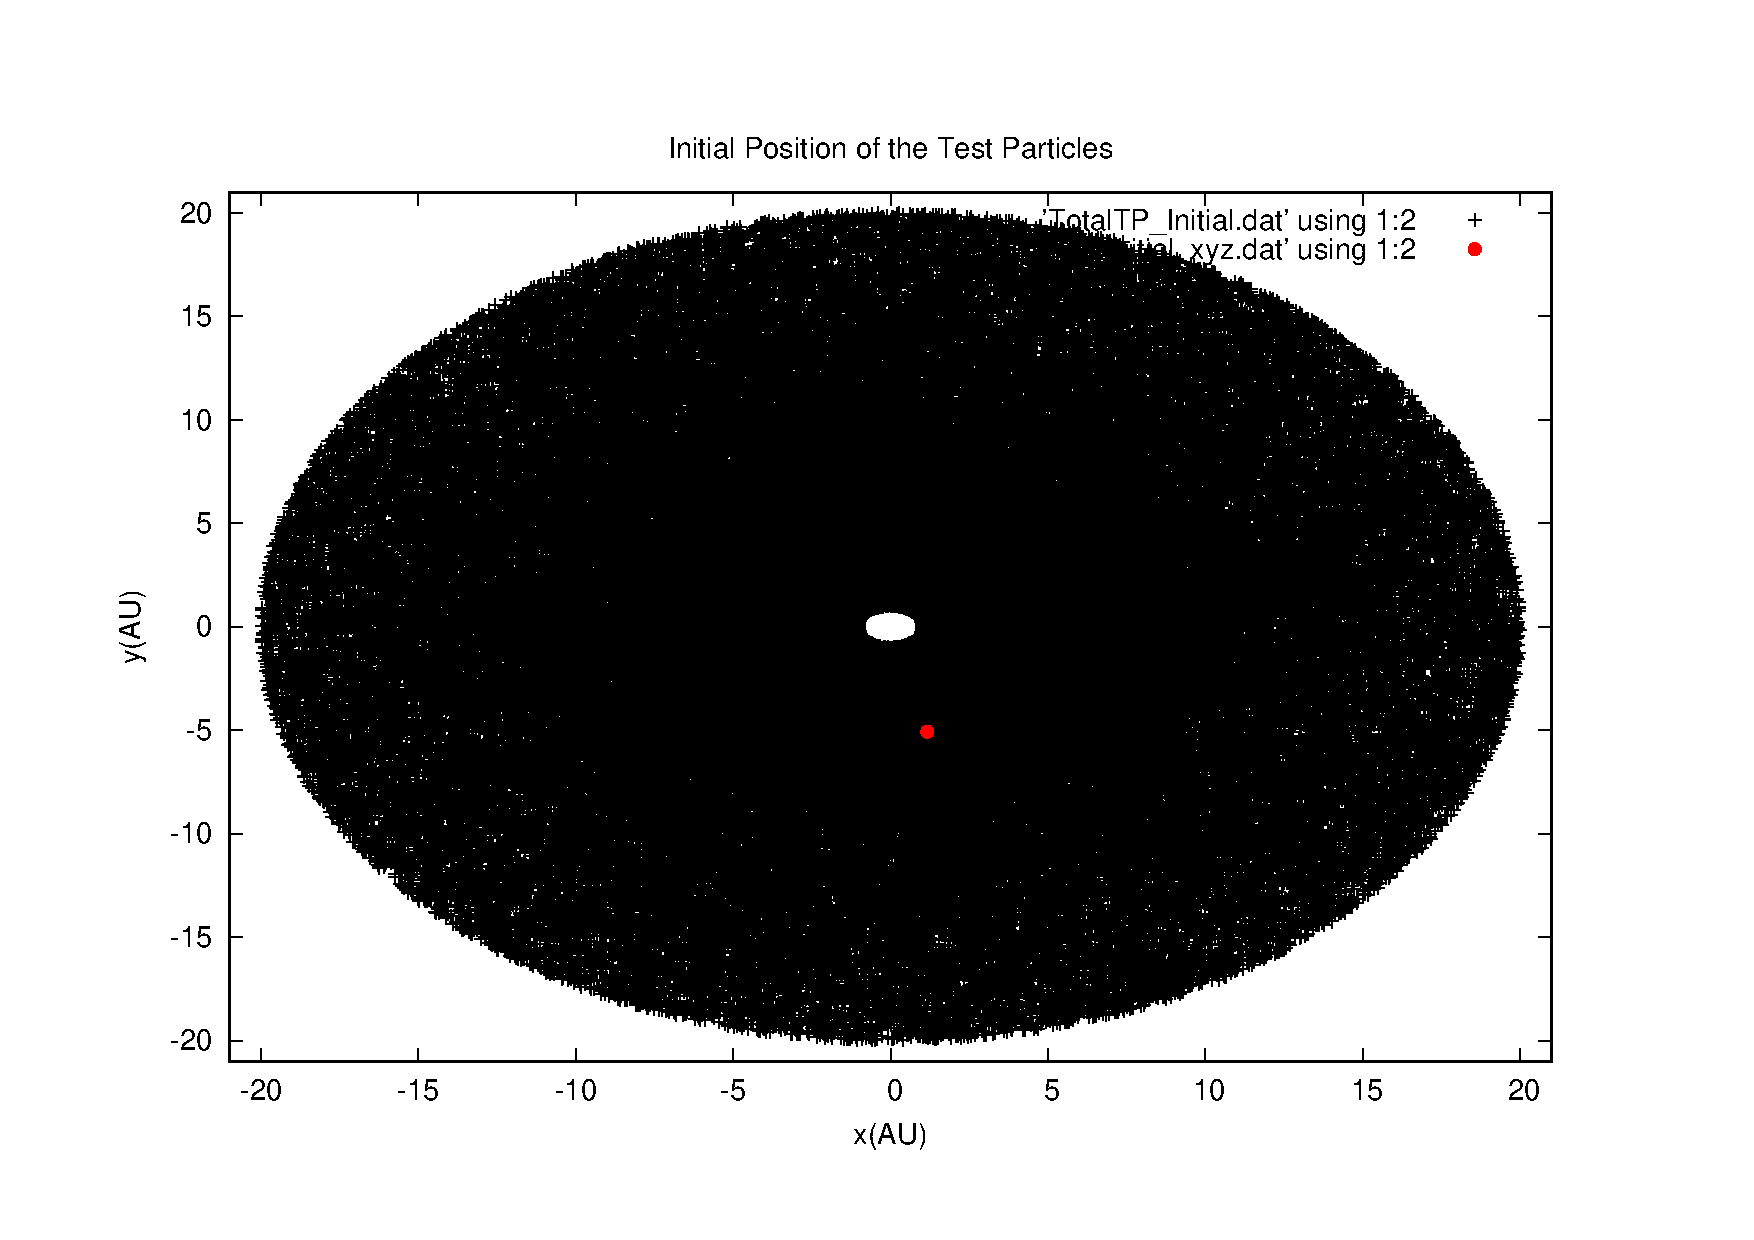
\includegraphics[scale= 0.5]{TotalTP_Initial}
  \caption{Δίσκος της Κατανομής των {\en Test Particles} τη Χρονική Στιγμή {\en $t_0=0 \; sec$ (Initial Disk)}}\label{InitialDisc:figure}
\end{figure}

Η θέση κάθε {\en test particle} στο επίπεδο συμβολίζεται με <<+>> , ενώ η θέση του πλανήτη με <<$\bullet$>>, η οποία στο παρόν γράφημα είναι κόκκινη για να ξεχωρίζει.\\

Λόγω των αρχικών συνθηκών που επιλέξαμε, ο δίσκος παρουσιάζει αξονική και κατοπτρική συμμετρία. Επίσης η {\it αριθμητική του πυκνότητα}, $N_{t_0=0}$, είναι σταθερή και γνωστή $\cdot$ καθώς έχουμε 6000 {\en test particles} σε καθε δακτύλιο πάχους 1 {\en AU}, οπότε μπορούμε να πούμε ότι η {\it επιφανειακή του πυκνότητα}, $\Sigma_{t_0=0}(r)$, μειώνεται συναρτήσει του τετραγώνου της απόστασης καθώς ο ίδιος αριθμός {\en test particles} διαμοιράζεται σε ολοένα και μεγαλύτερου εμβαδού δακτυλίους. Σαν αποτέλεσμα η {\it αριθμητική του πυκνότητα} και κατ' επέκταση η {\it επιφανειακή του πυκνότητα} προσδιορίζονται πλήρως απο τις αρχικές συνθήκες δημιουργίας του δίσκου (αν θεωρήσουμε δεδομένη την μάζα του κάθε {\en test particle}).

\newpage

\section{Παράμετροι της Σκόνης} 

Τα μικρά στερεά σωματίδια αποτελούν την σκόνη και προκειμένου να προσδιορίσουμε τα φυσικά χαρακτηριστικά της καταφύγαμε στις παρακάτω υποθέσεις και παραδοχές:

\begin{itemize}
\item Τα στερεά σωματίδια συγκροτούνται απο το ίδιο υλικό και έχουν ίδια χημική σύσταση, συγκεκριμένα απο $100\%$ πυριτικά άλατα, ({\en Astronomical Silicate}).
\item Τα στερεά σωματίδια θεωρήσαμε ότι είναι συμπαγή και έχουν σφαιρικό σχήμα ακτίνας $r_d$.
\item Τα στερεά σωματίδια χαρακτηρίζονται απο σταθερή πυκνότητα $\rho_d = 2.7 \frac{g}{cm^3}$
\end{itemize}

Οι πληροφορίες σχετικά με την σύσταση του υλικού και την πυκνότητα του πάρθηκαν απο το {\en Database of Optical Constants for Cosmic Dust}, \href{https://www.astro.uni-jena.de/Laboratory/OCDB/index.html}{[{\en OCDB}]}.\\

Στην συγκεκριμένη εργασία κάνουμε λόγο για έναν αρκετά μαζικό δίσκο σχετικά νεαρής ηλικίας και σύμφωνα με την λογική της παραγράφου (1.3.3) επιλέξαμε το μέγεθος των σωματιδίων της σκόνης να είναι λίγο μεγαλύτερο απο αυτό της {\en ISM}. Συνοψίζοντας τα παραπάνω, τα σωματίδια  που επιλέχθηκαν για την παρούσα εργασία είναι:

\begin{table}[h] 
 \centering
 \begin{tabular}{l | l | l | l}
      Ακτίνα ($r_d$) & Πυκνότητα ($\rho_d \; \frac{g}{cm^3}$) & Σύσταση\\
      \hline \hline
     $0.5$ μ$m$ & $2.7$ & $100\%$ πυριτικά άλατα\\
 \end{tabular}
 \caption{Οι Φυσικές Παράμετροι των Σωματιδίων της Σκόνης}\label{tab:ParticlesParameters}
\end{table}   

{\it Το κατώτατο όριο στο μέγεθος δεν είναι τυχαίο καθώς θεωρούμε ότι σωματίδια με ακτίνα $r_{d} < 0.45$ μ$m$ έχουν εκδιωχθεί απο το σύστημα λόγο της πίεσης της ακτινοβολίας του Ήλιου}!\cite{ertel2012observing}\\

Η μάζα του κάθε σωματιδίου ισούται με:

\begin{equation}\label{eq:ParticleMass}
 m=\frac{4 \pi \rho r_d^3 }{3} = 1.41372\times10^{-12} g
\end{equation}

Η συνολική μάζα του δίσκου είναι $M_{disk}= 10^{-4} M_{\odot}=1.99\times10^{29} g$ άρα η μάζα κάθε {\en test particle} είναι:

\begin{equation}\label{eq:InitialTPMass}
 m_{tp}=\frac{10^{-4} M_{\odot}}{114000} = 8.772\times10^{-10} M_{\odot} = 1.746\times10^{24}g
\end{equation}

Απο τις \eqref{eq:ParticleMass} και \eqref{eq:InitialTPMass} το κάθε {\en test particle} αντιπροσωπεύει $N$ σωματίδια, όπου:

\begin{equation}\label{eq:NbParticles}
 N=\frac{m_{tp}}{m}=\frac{1.746\times10^{24}}{1.41372\times10^{-12}} = 1.235\times10^{36}
\end{equation}

Τελικά ο δίσκος την χρονική στιγμή {\en $t_0=0 \; sec$} έχει μάζα $Μ_{disk}=1.99\times10^{29} g$ και περιέχει $N\times114000 = 1.407\times10^{41}$ σωματίδια σκόνης.\\






 

\chapter{Δυναμική Εξέλιξη του Συστήματος}

 \section{Προφιλ Επιφανειακής Πυκνότητας} 

 Η αριθμητική ολοκλήρωση έγινε για χρονικό διάστημα \textbf{\en 10Myrs}. Η επιλογή του χρονικού διαστήματος ολοκλήρωσης δεν είναι τυχαία, καθώς αντιστοιχεί  σε πολλές περιόδους περιφοράς του Δία. Με αυτό τον τρόπο εξασφαλίζουμε ότι θα μεσολαβήσει αρκετός χρόνος, ώστε τα αποτελέσματα που θα πάρουμε να είναι ασφαλή. Η ολοκλήρωση πραγματοποιήθηκε με βήμα $0.2 yrs$ παίρνοντας με αυτό τον τρόπο ικανοποιητικό αριθμό σημείων στις τροχιές των σωμάτων και εξήγαγε δεδομένα {\en (output)} κάθε $10^4 yrs$. Στη συνέχεια συντάχθηκε ένα {\en script} με την ονομασία {\en {\it xyToRTh.f}}, το οποίο μετέτρεπε τις Καρτεσιανές συντεταγμένες όλων των {\en test particles} του συστήματος σε Πολικές.\\
Αποτέλεσμα της αριθμητικής ολοκλήρωσης ήταν η δυναμική εξέλιξη του συστήματος για το χρονικό διάστημα των {\en 10Myrs}. Παρακάτω δίνεται η εικόνα του δίσκου:    

\begin{figure}[h]
  \centering
  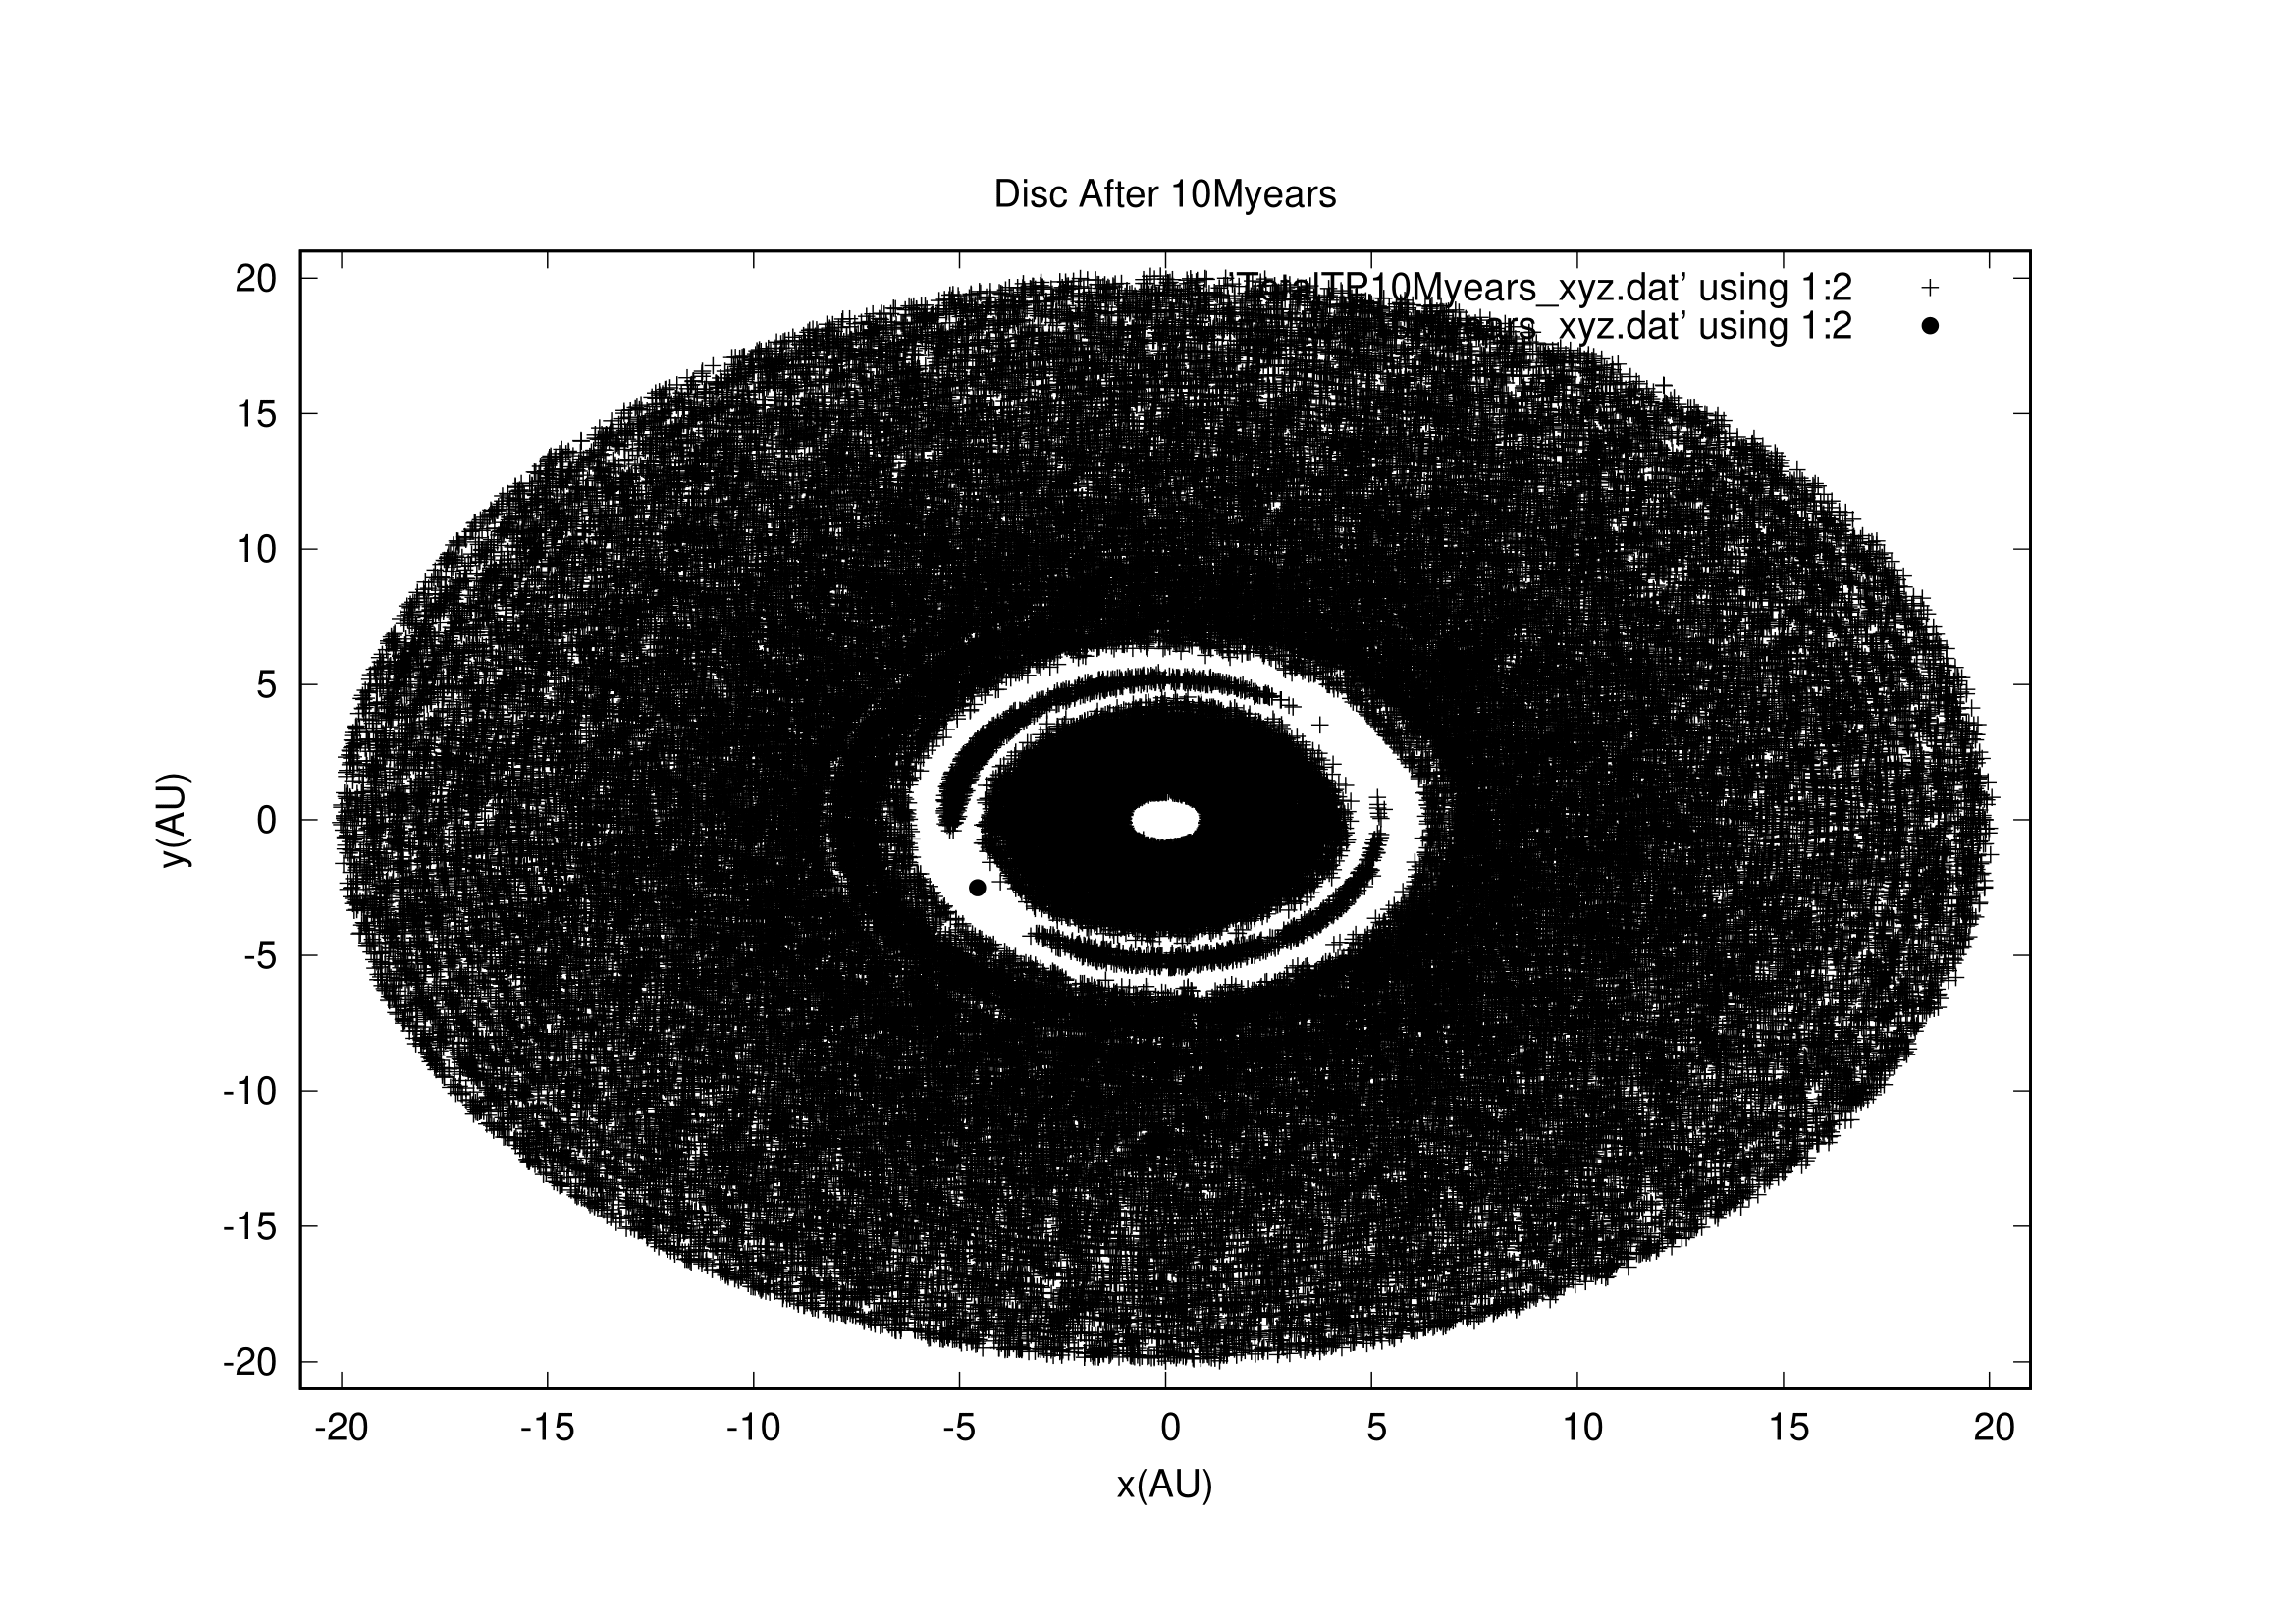
\includegraphics[scale=0.44]{TotalTP10Myears_xyz}
  \caption{Δίσκος τη Χρονική στιγμή $t_1=10 \; Myrs$}\label{fig:DiscAfter10Myear}
\end{figure}

Η θέση κάθε {\en test particle} που παρουσιάζεται στο επίπεδο $x-y$ συμβολίζεται με <<+>> , ενώ η θέση του Δία με <<$\bullet$>> και αυτός ο συμβολισμός θα τηρηθεί σε ολόκληρη την έκταση της εργασίας.\\


Αμέσως μετά την ολοκλήρωση της προσομοιώσης παρατηρούμε ότι:

\begin{itemize}
 \item O αριθμός των {\en test particles} του συστήματος έχει μειωθεί σε σχέση τον αρχικό τους αριθμό.
   \item Έχουν σχηματιστεί δύο ομάδες {\en test particles}, οι οποίες ακολουθούν την τροχιά του πλανήτη και οι θέσεις τους παρουσιάζουν συμμετρία ως προς αυτόν.
    \item Ο πλανήτης έχει <<καθαρίσει>> μεγάλο μέρος της τροχιάς του απο {\en test particles}, δημιουργώντας έναν κενό δακτύλιο στην επιφάνεια του δίσκου και αλλάζοντας έτσι το προφίλ της αριθμητικής του πυκνότητας.
\end{itemize}

\underline{\bf Ανάλυση των Παρατηρήσεων}
\vspace{0.3cm}   
   
Κατα το χρονικό διάστημα της ολοκλήρωσης τα {\en test particles} αλληλεπιδρούν βαρυτικά με τον αστέρα και τον πλανήτη. Αποτέλεσμα αυτής της αλληλεπίδρασης είναι η μεταβολή των στοιχείων της τροχιάς τους σύμφωνα με νόμους της Μηχανικής (όπως αναφέρθηκε ο πλανήτης δεν δέχεται την βαρυτική δύναμη της κατανομής). Έτσι κάποια {\en test particles} άλλοτε αποκτούν τροχιές που τους αναγκάζουν να πέσουνε στην επιφάνεια του αστέρα, άλλοτε ταχύτητες μεγαλύτερες απο την {\it ταχύτητα διαφυγής}\footnote{Ταχύτητα διαφυγής ή παραβολική ταχύτητα ονομάζεται η ελάχιστη ταχύτητα που πρέπει να αποκτήσει, ένα σώμα μάζας $m$ και απόστασης $r$ απο το ελκτικό κέντρο μάζας $Μ$, ώστε να τεθεί σε παραβολική τροχιά και να διαφύγει σε άπειρη απόσταση απο αυτό$\cdot$ $u_\infty = \sqrt{\frac{2G(M+m)}{r}}$} απο τον αστέρα και έτσι διαφεύγουν απο το σύστημα. Τελικά τα {\en test particles} αυτά  χαρακτηρίζονται {\en "not active"}. Ο {\en SWIFT} με τη χρήση του δισδιάστατου πίνακα $istat(NTPMAX,NSTAT)$ ελέγχει μετά απο κάθε {\en timestep} ποιά {\en test particles} είναι {\en "active"} και ποιά {\en "not active"}, καθώς συγκεκριμένοι δείκτες ενημερώνουν το πρόγραμμα σε ποία απο τις δύο καταστάσεις βρίσκεται το κάθε {\en test particle}. Τη χρονική στιγμή {\en $t_1=10 \; Myrs$} τα {\en test particles} που παραμένουν ενεργά στο σύστημα είναι 101294$\cdot$ άρα, απο την \eqref{eq:InitialTPMass}, μάζα του δίσκου είναι:

\begin{equation}\label{eq:t_1TPMass}
 M_{disk} =  101294\times1.746\times10^{24}g = 1.769\times10^{29} g
\end{equation} 
 
Οι δύο ομάδες των {\en test particles} που ακολουθούν την τροχιά του πλανήτη είναι σε συντονισμό $1:1$ με αυτόν και βρίσκονται στα {σημεία ευσταθούς ισορροπίας {\en Lagrange}} $L_4$ και $L_5$ του συστήματος πλανήτη-αστέρα\cite[{\en Chap.~3, Sect.~3.5-.3.7}]{murray1999solar}. Καθώς η τροχιά του πλανήτη είναι σχεδόν κυκλική τα τρίγωνα με κορυφές ΔΗ$L_4$ και ΔΗ$L_5$ είναι ισόπλευρα. Σαν αποτέλεσμα η μια ομάδα βρίσκεται δεσμευμένη σε ένα χώρο 60\degree ,($L_5$), πίσω απο τον πλανήτη (κινούμενη προς αυτόν) και η δεύτερη ομάδα βρίσκεται σε ένα χώρο 60\degree ,($L_4$), μπροστά του (ο πλανήτης κινείται προς αυτήν). Ο συγκεκριμένος συντονισμός είναι ευσταθής για χρόνους συγκρίσιμους με την ηλικία του σύμπαντος, οπότε αν δεν υπάρξει κάποια εξωτερική διαταραχή ο πλανήτης θα εξακολουθήσει να μοιράζεται την τροχιά του με τις δύο αυτές ομάδες διατηρώντας το σύστημα την γεωμετρία του. Οι δύο αυτές ομάδες  μπορούν να ταυτιστούν με τους γνωστούς {\it Τρωικούς} αστεροειδείς του Ηλιακού μας Συστήματος.\\
 
Το εύρος των κενού δακτυλίου {\en (gap)}, που δημιουργήθηκε στον δίσκο, εξαρτάται απο την {\it ακτίνα {\en Hill}} του πλανήτη,\eqref{eq:HillRadius}, άρα κατ' επέκταση απο τον λόγο της μάζας του προς τη μάζα του αστέρα. Ποιοτικά όσο μεγαλύτερη είναι η μάζα του πλανήτη τόσο μεγαλύτερο είναι και το εύρος του δακτυλίου που δημιουργεί στον δίσκο σκόνης. Για τον Δία στο συγκεκριμένο σύστημα μέσω της \eqref{eq:HillRadius} προκύπτει $r_H =0.82615${\en AU}.\\

Όπως αναφέραμε τη χρονική στιγμή {\en $t_0=0 \; sec$} η αριθμητική πυκνότητα των {\en test particles} του δίσκου, είναι σταθερή, οπότε μπορούμε να πούμε ότι η επιφανειακή του πυκνότητα μειώνεται συναρτήσει του τετραγώνου της απόστασης, αφού ο ίδιος αριθμός {\en test particles} διαμοιράζεται σε ολοένα και μεγαλύτερου εμβαδού δακτυλίους. Τη χρονική στιγμή όμως {\en $t_1=10 \; Myrs$} το προφίλ της αριθμητικής πυκνότητας (και κατεπέκταση της επιφανειακής πυκνότητας) του έχουν αλλάξει. Για να μελετήσουμε το νέο αυτό προφίλ αρχικά χωρίσαμε τον δίσκο σε δακτυλίους αριθμού $i$, πάχους $Dr$ και μετρήσαμε τον αριθμό {\en test particles} σε κάθε δακτύλιο συναρτήσει της απόστασης $r$ τους απο το ελκτικό κέντρο. Μέσα απο αυτό το γενικό <<σκανάρισμα>> εξάγαμε το γενικό προφίλ αριθμητικής πυκνότητας του δίσκου. Μετρήσεις έγιναν για τις τιμές:

\begin{table}[h]
 \centering
 \begin{tabular}{l | l | l}
      & $i$ & $Dr${\en (AU)}\\
      \hline \hline
    1 & 204 & 0.1\\
    2 & 120 & 0.17\\
    3 & 85 & 0.24\\          
 \end{tabular}
 \caption{Παράμετροι σκαναρίσματος για την εξαγωγή του γενικού προφίλ αριθμητικής πυκνότητας του δίσκου την {\en $t_1=10 \; Myrs$}}\label{tab:mytable4}
\end{table}

Παρακάτω δίνονται τα διαγράμματα, με τον αριθμό των {\en test particles} $N_{ri}$ συναρτήσει της απόστασης $r$, που προέκυψαν απο τις παραπάνω τιμές για κάθε ζεύγος τιμών:

\newpage

\begin{figure}[h] 
 \begin{subfigure}{0.48\textwidth}
  \includegraphics[width=\linewidth]{GeneralScan0,1}
  \caption{$i=204,Dr=0.1${\en AU}}\label{i204,Dr0.1}
 \end{subfigure}\hspace*{\fill}
 \begin{subfigure}{0.48\textwidth}
  \includegraphics[width=\linewidth]{GeneralScan0,1-Norm}
  \caption{$i=204,Dr=0.1${\en AU-Normalized}}\label{i204,Dr0.1 Norm}
 \end{subfigure}
 \medskip
  
 \begin{subfigure}{0.48\textwidth}
  \includegraphics[width=\linewidth]{GeneralScan0,17}
  \caption{$i=120,Dr=0.17${\en AU}}\label{i120,Dr0.17}
 \end{subfigure}\hspace*{\fill}
 \begin{subfigure}{0.48\textwidth}
  \includegraphics[width=\linewidth]{GeneralScan0,17-Norm}
  \caption{$i=120,Dr=0.17${\en AU-Normalized}}\label{i120,Dr0.17 Norm}
 \end{subfigure}
 \medskip
 
  \begin{subfigure}{0.48\textwidth}
   \includegraphics[width=\linewidth]{GeneralScan0,24}
   \caption{$i=85,Dr=0.24${\en AU}}\label{i85,Dr0.24}
  \end{subfigure}\hspace*{\fill}
  \begin{subfigure}{0.48\textwidth}
   \includegraphics[width=\linewidth]{GeneralScan0,24-Norm}
   \caption{$i=85,Dr=0.24${\en AU-Normalized}}\label{i85,Dr0.24 Norm}
  \end{subfigure}
 \caption{Γενικό Προφίλ Αριθμητικής Πυκνότητας της Κατανομής}
\end{figure}   
 
 Παρατηρώντας τα παραπάνω διαγράμματα μπορούμε να διακρίνουμε τις εξής περιοχές:
\begin{itemize}

 \item Για $0<r \leq 1 \; (AU)$ δεν υπάρχουν {\en test particles} και η αριθμητική πυκνότητα σε αυτή την περιοχή είναι μηδέν. 
 \item Στη συνέχεια για την περιοχή $1 \leq r \leq 3.85 \; (AU)$  ο αριθμος των {\en test particles} παρουσιάζει αύξηση, εκτός απο το σημείο που αντιστοιχεί σε  $r \simeq 3.4 (AU)$. 
 \item Μεταξύ των $3.85 \leq r \leq 7.5 \; (AU)$ εμφανίζεται μια μεγάλη κοίλη, η οποία διαχωρίζεται απο μια κορυφή για $r \simeq 5.2 (AU)$.
 \item O αριθμος των {\en test particles} για $ 7.5 \leq r \leq 20 \; (AU)$ είναι περίπου σταθερός εκτός απο το σημείο που αντιστοιχεί σε  $r \simeq 8.33 (AU)$. Απο εκεί και μετά ο αριθμός των {\en test particles} μειώνεται δραματικά καθώς έχουμε φτάσει στα πέρατα του δίσκου.
  
\end{itemize} 

\underline{\bf Ανάλυση των Διαγραμμάτων}
\vspace{0.3cm} 

Το γεγονός ότι στις περιοχές για $r_1 \simeq 3.4 (AU)$ και $r_2 \simeq 8.33 (AU)$ εμφανίζονται δύο {\it τοπικά ελάχιστα} στον αριθμό των {\en test particles} δεν είναι τυχαίο. Με βάση την \eqref{eq:ResonanceCondition2} παρατηρούμε ότι τα {\en test particles} με ${\en a}_1 \simeq 3.4 (AU)$ βρίσκονται πολύ κοντά στον συντονισμό 2:1 με τον πλανήτη και τα {\en test particles} με ${\en a}_2 \simeq 8.33 (AU)$ στον συντονισμο 1:2 με τον πλανήτη.

\begin{equation}\label{eq:ResonanceCondition3}
 (\frac{\alpha_1}{\alpha_J})^{3/2}=0.53 , \; (\frac{\alpha_J}{\alpha_2})^{3/2}=0.49    
\end{equation}

Οι συντονισμοί αυτοί είναι ασταθείς με αποτελέσμα τα {\en test particles} που βρίσκονται κοντά σε αυτούς να αποκτούν ασταθείς τροχιές σε σχετικά σύντομα χρονικά διαστήματα να μεταβάλλονται τα στοιχεία της τροχιάς τους. Ακόμα βλέπουμε ότι το <<πηγάδι>> στα διαγράμματα για τον συντονισμό τον 1:2, των {\en test particles} με τον πλανήτη, είναι βαθύτερο απο το πηγάδι για τον συντονισμό 2:1 με τον πλανήτη. Η συμπεριφορά αυτή ερμηνεύεται απο την \eqref{eq:ResonanceCondition3}, η οποία μας δείχνει ότι ο πρώτος είναι πιο κοντά στην ακριβή τιμή του συντονισμού, ($0.5$), άρα είναι και πιο ισχυρός.\\

Ουσιαστικά παρατηρώντας την γεωμετρία του δίσκου, Σχήμα:~\ref{fig:DiscAfter10Myear}, σε συνδυασμό με τα παραπάνω διαγράμματα αριθμητικής κατανομής των {\en test particles}, μπορούμε να κατανοήσουμε ότι η ενδιάμεση κορυφή αντιστοιχεί στις ομάδες {\en test particles} που εντοπίζονται στα {σημεία ευσταθούς ισορροπίας {\en Lagrange}} ($L_4$, $L_5$) και χρήζει πιο λεπτομερή ανάλυση.\\

Ας υποθέσουμε ότι κινούμαστε ακτινικά απο το κέντρο του δίσκου προς την άκρη του σε μια τυχαία διεύθυνση (τυχαία αζιμουθιακή γωνία θ)\footnote{Η γνωστή αζιμουθιακή γωνία των πολικών συντεταγμένων} έως ότου συναντήσουμε τα {\en test particles} των περιοχών $L_4$ και $L_5$ . Ακολουθώντας τον παραπάνω συλλογισμό είναι εμφανές ότι καθώς κινηθούμε ακτινικά το {\bf αν} θα τα συναντήσουμε {\it εξαρτάται απο την γωνία θ} στην οποία θα επιλέξουμε να κινηθούμε$\cdot$ καθώς η δακτυλοειδής αυτή περιοχή, σε αντίθεση με τις άλλες δύο, δεν είναι συνεχής αλλά διαχωρίζεται στη διάμετρο που ταυτίζεται με την διεύθυνση εντοπισμού του πλανήτη. Η ύπαρξη της ενδιάμεσης αυτής κορυφής, σε συνδυασμό με τον κενό δακτύλιο, θα μας απασχολίσει ιδιαίτερα καθώς αποτελούν την \underline{\bf{ ένδειξη ύπαρξης πλανήτη}} στον δίσκο. Τέλος τα δύο <<πηγάδια>> δεξιά και αριστερά της ενδιάμεσης κορυφής αντιστοιχούν στον κενό δακτύλιο που δημιουργεί ο πλανήτης στην τροχία του. Ο δακτύλιος αυτός, προφανώς δεν είναι απόλυτα κενός, αλλα περιέχει τα {\en test particles} των περιοχών $L_4$, $L_5$ για αυτό και εμφανίζεται η κορυφή όπως αναφέρθηκε.\\

Το γεγονός ότι για αποστάσεις $r > 8.33 (AU)$ η αριθμητική πυκνότητα των {\en test particles} είναι σχεδόν σταθερή μας σηματοδοτεί και το όριο της κυριαρχίας του βαρυτικού δυναμικού του Δία. Φυσικά η βαρυτική του δύναμη εξακολουθεί να ασκείται στα {\en test particles} όμως δεν είναι ικανή να μεταβάλλει έντονα τα στοιχεία της τροχιάς τους$\cdot$ εκτός για κάποια απο αυτά που ίσως βρεθούν σε κάποιο συντονισμό ασταθούς ισορροπίας με τον Δία.\\

Στο σημείο αυτό προκειμένου να μελετήσουμε σε μεγαλύτερο βάθος την γεωμετρία που απέκτησε ο δίσκος λόγω της παρουσίας του πλανήτη, αλλα και τις χαρακτηριστικές περιοχές της κατανομής, συντάχθηκε ένα {\en script} με την ονομασία {\en {\it ScanDiskFixed.f}}. Σύμφωνα με αυτό χωρίσαμε επιπλέον τον δίσκο, με αρχή την διεύθυνση του πλανήτη την {\en $t_1=10 \; Myrs$} , σε ${\en j=36}$ διαμετρικές διευθύνσεις ανα 10\degree \; και επαναλάβαμε την διαδικασία <<σκαναρίσματος>> του δίσκου δοκιμάζοντας διαφορετικές τιμές παραμέτρων. Έστω πχ η διεύθυνση αναφοράς είναι η θ$=0\degree$ και θ$=180\degree$, η επόμενη είναι η θ$=10\degree$ και θ$=190\degree$ κ.ο.κ.\\
Τώρα μετρήθηκε ο αριθμός {\en test particles} σε κάθε διεύθυνση με εύρος $\pm$ $Dth\degree$, σε κάθε έναν δακτυλίο πάχους $Dr$ απο τους $i$ δακτυλίους. Ισοδύναμα  μετρήθηκε ο αριθμός των {\en test particles} σε κάθε <<κελί>> $[i,j]$, όπου $i=1,2,3,..$ και $j=1,2,3,...,36$. Μετρήσεις έγιναν για τις τιμές:

\begin{table}[h]
 \begin{subtable}[h]{0.3\textwidth}
   \centering
   \begin{tabular}{l | l | l}
      & $i$ & $Dr${\en (AU)}\\
    \hline \hline
    1 & 204 & 0.1\\
    2 & 120 & 0.17\\
    3 & 85 & 0.24\\
    \end{tabular}
    \caption{$Dth=\pm$ $10\degree$}\label{tab:+-10degree}
 \end{subtable}
 \hfill      
 \begin{subtable}[h]{0.3\textwidth}
   \centering
   \begin{tabular}{l | l | l}
      & $i$ & $Dr${\en (AU)}\\
    \hline \hline
    1 & 204 & 0.1\\
    2 & 120 & 0.17\\
    3 & 85 & 0.24\\
    \end{tabular}
    \caption{$Dth=\pm$ $15\degree$}\label{tab:+-15degree}  
  \end{subtable}
  \hfill  
 \begin{subtable}[h]{0.3\textwidth}
   \centering
   \begin{tabular}{l | l | l}
      & $i$ & $Dr${\en (AU)}\\
    \hline \hline
    1 & 204 & 0.1\\
    2 & 120 & 0.17\\
    3 & 85 & 0.24\\
    \end{tabular}
    \caption{$Dth=\pm$ $20\degree$}\label{tab:+-20degree}   
 \end{subtable}
\caption{Τιμές των Διαφόρων Παραμέτρων <<Σκαναρίσματος>> του Δίσκου}\label{tab:Scans}
\end{table}

Είναι φανερό ότι οι 36 διευθύνσεις ανα $10\degree$ έχουν σαν αποτέλεσμα να μετρηθεί δύο φορές ο αριθμός των {\en test particles} του δίσκου. Επιπλέον το εύρος $\pm$ $Dth\degree$ σε κάθε διεύθυνση έχει σαν αποτέλεσμα επικαλύψεις μεταξύ των περιοχών μέτρησης {\en test particles}. Για τους παραπάνω λόγους ο αριθμός των {\en test particles} κανονονικοποιήθηκε σύμφωνα με το εμβαδόν επικάλυψης για τα διαφορετικά εύρη <<σκαναρίσματος>>. Επίσης κρατήσαμε τις μετρήσεις των 18 πρώτων διαμετρικών διευθύνσεων, ($j=1,2,3,...,18$), καθώς αύτες περιλαμβάνουν μια πλήρη μέτρηση των {\en test particles} του δίσκου ($18\times10\degree=180\degree$) και οι επόμενες 18 είναι αντίστοιχες καθώς μετριούνται τα {\en test particles} του δίσκου για δεύτερη φορά.

Καταλήξαμε να κρατήσουμε τις τιμές των παραμέτρων που δίνουν τον διαχωρισμό του δίσκου σε $i=120$ δακτυλίους πάχους $Dr=0.17${\en AU}, δηλαδή 

\begin{table}[h]
 \centering
 \begin{tabular}{l | l | l}
     $\pm$ $Dth\degree$ & $i$ & $Dr${\en (AU)}\\
      \hline \hline
    $\pm$ 10 & 120 & 0.17\\
    $\pm$ 15 & 120 & 0.17\\
    $\pm$ 20 & 120 & 0.17\\      
 \end{tabular}
 \caption{Παράμετροι Διαχωρισμού του Δίσκου- <<Σκαναρισματος>>}\label{tab:ScanParameters}
\end{table}

 Τελικά πήραμε 54 διαφορετικές μετρήσεις του αριθμού των {\en test particles} για κάθε <<κελί>> ενός δακτυλίου $Dr_i$, όπου $i=1,2,...,120$. Στη συνέχεια βρήκαμε τον {\it μέσο όρο του αριθμού των {\en test particles}}, $Mean N_{ri}$, για κάθε <<κελί>> δακτυλίου $i$ και πάχους $Dr_i$ καθώς και το <<κελί>> με τον μέγιστο αριθμό {\en test particles}, $N_{max}$, και αυτό με τον ελάχιστο αριθμό {\en test particles}, $N_{min}$. Παρακάτω δίνεται η γραφική παράσταση μαζί με την {\it τυπική απόκλιση} των μετρήσεων στον μέσο όρο:
 \newpage

\begin{figure}[h]
  \centering
  \includegraphics[scale=0.5]{MeanNumDensity}
  \caption{Μέσος Όρος του Αριθμού των {\en Test Particles} σε κάθε Δακτύλιο $Dr_i$\\
  Με κόκκινο χρώμα δίνεται η $N_{max}(r)$, με πράσινο η $N_{min}$ και ο $Mean N$ μπλέ}\label{fig:MeanNb}
\end{figure}  

Βλέπουμε ότι σε κάθε δακτύλιο $r_i$, \underline{με εξαίρεση την περιοχή του πλανήτη}, οι τιμές της {\it τυπικής απόκλισης} δεν είναι μεγάλες, αυτό σημαίνει ότι η διαφορά του αριθμού των {\en test particles} μεταξύ των <<κελιών>> με το ίδιο $r$ αλλά διαφορετική διεύθυνση θ (πχ τα <<κελιά>> [3,1],[3,2],[3,3] κ.ο.κ.) δεν είναι μεγάλη ή ισοδύναμα έχουμε περίπου ομοιόμορφα κατανεμημένα τα {\en test particles} του κάθε δακτυλίου σε αυτόν και ο συνολικός τους αριθμός μπορει να προσεγγιστεί αρκετά ικανοποιητικά απο τον μέσο όρο $MeanN_{ri}\forall i=1,2,...,120$. Αντίθετα ο αριθμός των {\en test particles}, για $r$ κοντά στην $r_J = 5.2044${\en AU}, παρουσιάζει μεγάλη διασπορά τιμών$\cdot$ σε κάποια διεύθυνση ο αριθμός των {\en test particles} αγγίζει το μηδέν ενώ ταυτόχρονα ο αριθμός {\en test particles} σε άλλη διεύθυνση παρουσιάζει μεγάλες τιμές. Αυτή ακριβώς η μη ισοτροπική κατανομή των {\en test particles} στη συγκεκριμένη απόσταση $r$ αποτελεί ένδειξη ότι υπάρχει ένα μαζικό σώμα σε αυτήν περίπου την απόσταση. Η παρουσία του σώματος και κατ' επέκταση η βαρυτική του επιρροή προκαλεί την μεγάλη διασπορά στον αριθμό των {\en test particles}, η οποία αντίστροφα είναι η δυναμική <<υπογραφή>> της παρουσίας του.\\

\newpage

Με δεδομένο το προφίλ αριθμητικής πυκνότητας του δίσκου μπορούμε να εξάγουμε και το προφίλ της επιφανειακής του πυκνότητας, αφού γνωρίζουμε εμβαδόν κάθε δακτυλίου και την μάζα του καθε {\en test particle}. Παρακάτω δίνεται το διάγραμμα επιφανειακής πυκνότητας του δίσκου:


\begin{figure}[h]
  \centering
  \includegraphics[scale=0.5]{SurfDens(units)}
  \caption{Επιφανειακή Πυκνότητα σε κάθε Δακτύλιο $Dr_i$ Συναρτήσει της Απόστασης\\
  Με κόκκινο χρώμα δίνεται η $\Sigma_{max}(r)$, με πράσινο η $\Sigma_{min}(r)$ και ο $\Sigma(r)$ μπλέ}\label{fig:SurfDens}
\end{figure}

Φαίνεται καθαρά η {\it εκθετική μείωση} της επιφανειακής πυκνότητας συναρτήσει της απόστασης μέχρι το όριο όπου το βαρυτικό δυναμικό του πλανήτη παύει να παίζει τον κυρίαρχο ρόλο. Απο εκεί και μετά η καμπύλη της επιφανειακής πυκνότητας είναι πιο ομαλή και συνεχίζει να μειώνεται συναρτήσει της απόστασης με μικρότερο όμως ρυθμό. Επίσης φαίνονται καθαρά τα δύο τοπικά ελάχιστα που αντιστοιχούν στους μεγάλους ημιάξονες $\alpha_1 \simeq 3.4 (AU)$ και $\alpha_2 \simeq 8.33 (AU)\cdot$ καθώς τα {\en test particles} βρίσκονται πολύ κοντά στους συντονισμούς 2:1 και 1:2 με τον πλανήτη.\\

Στο σημείο αυτό αξίζει να σημειωθεί ότι το 55.25\% της συνολικής μάζας του δίσκου βρίσκεται μεταξύ $1$ με $~5 AU$, δηλαδή σε έναν δακτύλιο εύρους $~4AU$. Το υπόλοιπο 44.75\% κατανέμεται απο $~5$ εώς $20.4 AU$, δηλαδή σε ένα δακτύλιο εύρους $~15AU$. Αυτή η μεγάλη διαφοροποίηση στην επιφανειακή πυκνότητα του δίσκου θα είναι πολύ σημαντική για τα αποτελέσματα του μοντέλου μας όπως θα δούμε παρακάτω.\\

Τέλος για να προσδιορίσουμε την αντίστοιχη καμπύλη, \ref{eq:SurfaceProfile}, που περιγράφει το προφίλ επιφανειακής πυκνότητας του δίσκου βάση των δεδομένων μας αποβάλλαμε τους δακτυλίους απόστασης $<1 AU$, καθώς δεν εμπεριέχουν καθόλου ύλη. Παρακάτω δίνεται το διάγραμμα επιφανειακής πυκνότητας του δίσκου για $r \geq1 AU$:

\begin{figure}[h]
  \centering
  \includegraphics[scale=0.5]{SurfDens(units)2}
  \caption{Επιφανεικαή Πυκνότητα σε κάθε Δακτύλιο $Dr_i$, όπου $r \geq1 AU$ Συναρτήσει της Απόστασης\\
  Με κόκκινο χρώμα δίνεται η $\Sigma_{max}(r)$, με πράσινο η $\Sigma_{min}(r)$ και ο $\Sigma(r)$ μπλέ}\label{fig:SurfDens2}
\end{figure}

όπου τελικά $\Sigma(r) = 8.53889\times r^{-1.20529} \frac{g}{cm^2}$.




\chapter{Κατανομή της Εκπεμπόμενης Ακτινοβολίας}
 Προκειμένου να υπολογίσουμε την {\it Θερμοκρασία Ισορροπίας} των σωματιδίων της σκόνης στον δίσκο πρέπει αρχικά να ορίσουμε τα χαρακτηριστικά του πεδίου της ακτινοβολίας. 

\section{Επιλογή Πεδίου Ακτινοβολίας}

Στο σημείο αυτό ας θεωρήσουμε ως πεδίο ακτινοβολίας ένα αστέρι και την γύρω περιοχή του. Φυσικά δε μπορούμε να έχουμε αυστηρά συνθήκες θερμοδυναμικής ισορροπίας καθώς οι φυσικές παράμετροι, όπως η θερμοκρασία, μεταβάλλονται στον χώρο και στον χρόνο. Μπορούμε όμως να υποθέσουμε συνθήκες {\it τοπικής θερμοδυναμικής Ισορροπίας} για μεταβολές αρκετά μικρές, σε κλίμακες συγκρίσιμες με την μέση ελεύθερη διαδρομή των φωτονίων. Έτσι υποθέτουμε ότι {\it η επιφάνεια του αστέρα εκπέμπει ακτινοβολία σαν μέλαν σώμα} \\

Στην παρούσα εργασία επιλέξαμε σαν κεντρικό άστρο τον Ήλιο. Θεωρώντας σφαιρική συμμετρία και απο την σχέση \eqref{eq:TotalPossitiveFlux} η συνολική θετική ροή που εκπέμπεται από την επιφάνεια του προς όλες τις κατευθύνσεις δίνεται απο την σχέση \eqref{eq:TotalPossitiveFlux}:

\begin{equation}\label{eq:SunsTotalPosFLux}
  F^{+} =\sigma T_{e}^4, \text{όπου $T_{e}$ η ενεργός θερμοκρασία της επιφάνεις του Ήλιου}
\end{equation}  

Η συνολική ηλεκτρομαγνητική ισχύς ή αντίστοιχα η ενέργεια ανα μονάδα χρόνου που εκπέμπει ο Ήλιος απο την επιφάνεια του σε όλο το ηλεκτρομαγνητικό φάσμα ονομάζεται {\it Φωτεινότητα}, $L_\odot$ και προφανώς: 

\begin{equation}\label{eq:Brightness}
  L_\odot = 4\pi R_{\odot}^2 F^{+} = 4\pi R_{\odot}^2 \sigma T_{e}^4 , \; \frac{erg}{sec}
\end{equation}

H φαινόμενη λαμπρότητα του Ήλιου, $l_\odot$ που ονομάζεται {\it Ηλιακή Σταθερά}, είναι γνωστή απο αστρονομικές παρατηρήσεις. Η φαινόμενη λαμπρότητα ουσιαστικά ισούται με την φωτεινότητα $L_\odot$ διαμοιρασμένη σε μια επιφάνεια σφαίρας με ακτίνα την απόσταση Γης-Ήλιου.

\begin{equation}\label{eq:Brightness2}
  L_\odot = 4\pi (1 AU)^2 l_\odot,  \; \frac{erg}{sec}
\end{equation}

Απο τις \eqref{eq:SunsTotalPosFLux}, \eqref{eq:Brightness} και \eqref{eq:Brightness2} προκύπτει:

\begin{align}
  T_{e}^4 = \frac{4\pi (1 AU)^2 l_\odot}{4\pi R_{\odot}^2 \sigma} \nonumber \\
  T_{e}^4 = \frac{(1 AU)^2 l_\odot}{R_{\odot}^2 \sigma} \nonumber \\
  T_{e} = 5777.62 K \label{eq:SunsTemp}
\end{align}

Απο τον νόμο του {\en Wien}, \eqref{eq:WienLaw}, προκύπτει ότι το μέγιστο της εκπεμπόμενης ηλιακής ακτινοβολίας εντοπίζεται στα $\lambda_{max}=0.5016$ μ$m$, δηλαδή στην περιοχή του {\it Ορατού} τμήματος του ηλεκτρομαγνητικού φάσματος. Τελικά απο τις σχέσεις \eqref{eq:SunsTotalPosFLux} και \eqref{eq:Brightness} προκύπτει η φωτεινότητα του Ήλιου είναι:

\begin{equation}\label{eq:Brightness3}
  L_\odot = 3.8412 \times 10^{33} \; \frac{erg}{sec}
\end{equation}


\section{Υπολογισμός της Θερμοκρασίας Ισορροπίας της Σκόνης του Δίσκου}

Για να υπολογίσουμε την {\it Θερμοκρασία Ισορροπίας}, $T_{dust}$ της σκόνης πρέπει να πρώτα να συνυπολογίσουμε τον ρυθμό θέρμανσης και ψύξης ($H = \frac{erg}{sec}$ και $C= \frac{erg}{sec}$ αντίστοιχα) του κάθε σωματιδίου. Ο ρυθμός θέρμανσης ενός σωματιδίου σκόνης ισοδύναμεί με την ενέργεια που απορροφάει το σωματίδιο, ανα μονάδα χρόνου, απο τα φωτόνια όλων των συχνοτήτων του φάσματος προερχόμενα απο όλες τις διευθύνσεις.

\begin{equation}\label{eq:HeatingRate}
H =  \int_{0}^{\infty} k_{\nu} \pi J_{\nu} d\nu 
\end{equation}

Στο σημείο αυτό υποθέτουμε ότι κάθε στερεό σωματίδιο δέχεται απευθείας την ηλιακή ακτινοβολία, χωρίς δηλαδή κάποιο άλλο σωματίδιο να βρισκεται μπροστά του και να αποκόπτει μέρος αυτής ({\en optically thin Disc}). Τελικά κάθε σωματίδιο σκόνης θερμαίνεται αποκλειστικά απο την ακτινοβολία του Ήλιου\footnote{Aγνοούμε την ενέργεια που μπορεί να απορροφήσει ένα σωματίδιο απο τα υπόλοιπα σωματίδια, καθώς όλα εκπέμπουν προς όλες τις κατευθύνσεις ($4\pi$)}.\\

Ο Ήλιος για ένα σωματίδiο απόστασης, $r$, υπόκειται σε στερέα γωνία $\pi \frac{R_{\odot}^2}{r^2}$ και η είδικη ένταση της ακτινοβολίας που δέχεται το σωματίδιο είναι $B_{\nu}(T_{e})$. Απο την σχέση \eqref{eq:MeanIntensity} η μέση ένταση που δέχεται απο όλες τις διευθύνσεις (εντός της στερεάς γωνίας, $\pi \frac{R_{\odot}^2}{r^2}$) είναι:

\begin{equation}\label{eq:ParticleMeanIntensity}
 J_{\nu}=\frac{\pi R_{\odot}^2}{4 \pi r^2} B_{\nu}(T_{e}), \; \frac{erg}{sec \; cm^2 \; Hz \; ster} 
\end{equation}

Τελικά απο τις \eqref{eq:HeatingRate} και \eqref{eq:ParticleMeanIntensity} προκύπτει:

\begin{equation}\label{eq:HeatingRate2}
H = \frac{4(\pi r_{d})^2}{4m} (\frac{R_{\odot}}{r})^2 \int_{0}^{\infty} Q_{\nu}B_{\nu}(T_{e}) d\nu  
\end{equation}

Ο ρυθμός ψύξης ενός σωματιδίου ισοδύναμεί με την ενέργεια που εκπέμπει το σωματίδιο, ανά μονάδα χρόνου, για τα φωτόνια όλων των συχνοτήτων του φάσματος προς όλες τις κατευθύνσεις:

\begin{equation}\label{eq:CoolingRate2}
C = \int_{0}^{\infty} k_{\nu} \pi B_{\nu}(T_{dust}) d\nu = \frac{4(\pi r_{d})^2}{m} \int_{0}^{\infty} Q_{\nu}^{emis} B_{\nu}(T_{dust}) d\nu  
\end{equation}

Υποθέτωντας ότι μετά απο κάποιο χρονικό διάστημα τα σωματίδια της σκόνης, θερμοκρασίας $T_{dust}$, βρίσκονται σε θερμοδυναμική ισορροπία θα πρέπει ο ρυθμός ψύξης, $C$, να ισούται με τον ρυθμό θέρμανσης, $H$. Η παραπάνω υπόθεση προέρχεται απο τον Νόμο του {\en Kirchhoff} και κατ' επέκταση συμπεραίνουμε ότι όση ακτινοβολία απορροφάται τόση εκπέμπεται άρα μπορούμε να αντικαταστήσουμε στον ρυθμό ψύξης την αποδοτικότητα εκπομπής, $Q_{\nu}^{emis}$ \footnote{Η φυσική σημασία της αποδοτικότητας εκπομπής είναι ανάλογη με αυτήν την αποδοτικότητας απορρόφησης, όπως ορίστηκε, για την διαδικασία όμως της εκπομπής του φωτός. Συνήθως συμβολίζονται $Q_{\nu}^{emis}$ και $Q_{\nu}^{abs}$ αντίστοιχα, αλλα στην εργασία χρησιμοποιούμε $Q_{\nu}^{emis}$ και $Q_{\nu}$, με την  αποδοτικότητα απορρόφησης, $Q_{\nu}$}. Τελικά απο την σχέση $H=C$ έχουμε:

\begin{equation}\label{eq:CalcTdust}
(\frac{R_{\odot}}{2r})^2 \int_{0}^{\infty} Q_{\nu} B_{\nu}(T_{e}) d\nu = \int_{0}^{\infty} Q_{\nu} B_{\nu}(T_{dust}) d\nu 
\end{equation}

Στο σημείο αυτό θα γίνει μια ποιοτική ανάλυση για την λύση των δύο ολοκλήρωμάτων.\\
Όσον αφορά το ολοκλήρωμα στο αριστερό κομμάτι γνωρίζουμε ότι ο Ήλιος δεν εκπέμπει αποτελεσματικά στα μεγάλα μήκη κύματος,($\lambda_{IR}$ έως $\lambda = \infty$) $\cdot$ επίσης η σκόνη δεν απορροφά καθόλου στα πολύ μικρά μήκη κύματος,($\lambda = 0$ έως $\lambda_{UV}$). Τέλος τα μήκη κύματος, τα οποία είναι σχετικά με την αποτελεσματική απορρόφηση,($\lambda_{UV}$ έως $\lambda_{IR}$), είμαστε στο όριο της γεωμετρικής οπτικής οπότε μπορούμε να υποθέσουμε $Q_{\nu}=1$.\\
Όσον αφορά το ολοκλήρωμα στο δεξί κομμάτι γνωρίζουμε ότι η σκόνη εκπέμπει αποτελεσματικά στα μεγάλα μήκη κύματος όπου βρισκόμαστε στο όριο {\en Rayleigh} και ο συντελεστής $Q_{\nu}$ δίνεται απο τη σχέση \eqref{eq:AbsorEfficiency}.
Έτσι απο τις \eqref{eq:CalcTdust}, \eqref{eq:TotalInteBlackBody}, \eqref{eq:Brightness} για το αριστερό μέλος της ισότητας και απο την λύση του δεξιού μέλους της εξίσωσης\cite[{\en Chap.~8, Sect.~2.2}]{krugel2002physics} προκύπτει:

\begin{equation}
\frac{L_\odot}{16 (\pi r_d)^2} = 1.47\times10^{-6} r_d T_{dust}^6, \; \text{για $\beta=2$ και οι μονάδες είναι $r$ και $r_d$ se $cm$} 
\end{equation}

Μετατρέποντας την απόσταση $r$ σε $AU$ και για $r_d = 0.5$μ$m =5\times10^{-5} cm$ τελικά προκύπτει:

\begin{equation}\label{eq:DustTemp}
T_{dust} = 377.54 r^{- \frac{1}3}, \; \text{για $\beta=2$} 
\end{equation}

Η εξίσωση \eqref{eq:DustTemp} δίνει την θερμοκρασία ισορροπίας των {\en test particles} και κατ' επέκταση των σωματιδίων της σκόνης συναρτήσει της απόστασης.

\newpage
Παρακάτω δίνεται θερμοκρασία ισορροπίας των {\en test particles} (και κατ' επέκταση των σωματιδίων της σκόνης) συναρτήσει της απόστασης στον δίσκο, αλλά και η μέση θερμοκρασία κάθε δακτυλίου $i, i=1,2,3,...,120$ του δίσκου:

\begin{figure}[h]
\centering
 \begin{subfigure}{0.48\textwidth}
  \includegraphics[width=\linewidth]{T_dust}
  \caption{Θερμοκρασία των {\en test particles} συναρτησει της απόστασης τους}\label{fig:TPTemp}
 \end{subfigure}\hfill
 \begin{subfigure}{0.48\textwidth}
  \centering
  \includegraphics[width=\linewidth]{T_dustRi}
  \caption{Μέση θερμοκρασία κάθε δακτυλίου συναρτησει της απόστασης του}\label{fig:DiscTemp}
 \end{subfigure}
\end{figure}

Στο διάγραμμα \ref{fig:TPTemp} εντοπίζουμε δύο περιοχές όπου δεν υπάρχουν {\en test particles}. Φυσικά οι περιοχές αυτές αντιστοιχούν στον κενό δακτυλίο που έχει δημιουργήσει ο Δίας καθώς περιφέρεται στην τροχία του. Ακόμα στο διάγραμμα \ref{fig:DiscTemp} πρέπει να σημειωθεί ότι τα πρώτα 5 σημεία αντιστοιχούν στους δακτυλίους μέσης απόστασης $r_i =i\times0,17 AU$ με $i=1,2,3,4,5$ στους οποίους δεν εμπεριέχονται σωματίδια. Το γεγονός γίνεται φανερό και απο το διαγράμμα \ref{fig:TPTemp}, όπου τα {\en test paticles} εντοπίζονται απο αποστάσεις $r \geq 1AU$. Τέλος η εξίσωση \eqref{eq:DustTemp} δίνει ικανοποιητικά αποτελέσματα για σωματίδια διαμέτρου μέχρι $~1$μ$m$.\\









\chapter{Φασματική και Χωρική Κατανομή της Εκπεμπόμενης Ακτινοβολίας}
\section{Φασματική Κατανομή της Ισχύος}

Ο δίσκος θερμοκρασίας $Τ_{dust}$ βρίσκεται σε Θερμοδυναμική Ισορροπία και ακτινοβολεί. Θέλουμε να βρούμε την φασματική κατανομή της ενέργειας του δίσκου, ({\en SED}),  που λαμβάνει παρατηρητής σε απόσταση $D=100 \; pc$ απο τον δίσκο βλέποντας τον {\en ``face on``}, δηλαδή στην \eqref{eq:SpecificIntensity} $\theta=0\deg$. H {\en SED} είναι ένα διάγραμμα $\lambda F_{\lambda}$ {\en vs} $\lambda$, το οποίο χρησιμοποιείται ευρέως για τον χαρακτηρισμό αστρονομικών πηγών.\\
Προκειμένου να υπολογίσουμε την {\en SED} συντάχθηκε ένα {\en script} με την ονομασία {\en {\it System'sSED.py}}, όπου θεωρήσαμε ότι κάθε δακτύλιος του δίσκου αντιπροσωπέυει ένα {\en ``pixel``} πάχους $Dr=0.17AU$. Έτσι το σύνολο των σωματιδίων κάθε δακτυλίου $i=1,2,...,120$, πάχους $Dr_i$, επιφανειακής πυκνότητας $\Sigma_{ri}$ και θερμοκρασίας $Τ_{ri}$ αντιπροσωπεύουν ένα <<μεγάλο σωματίδιο>>.  Ο παρατηρητής σε απόσταση $D$ απο τον δίσκο λαμβάνει, απο κάθε δακτύλιο $i$, μονοχρωματική ροή ακτινοβολίας $F_{\lambda}^i$ (ή $F_{\nu}^i$ αντίστοιχα). Θεωρούμε την ακτινοβολία πίσω απο τον δίσκο αμελητέα$\cdot$ έτσι απο τις σχέσεις \eqref{eq:RadiationTransferEquation4}, \eqref{eq:RadiationTransferEquationBlackBody}, \eqref{eq:SpecInteBlackBody} και \eqref{eq:SpecInteBlackBody2} προκύπτει:

\begin{align}
 F_{\lambda}^i = (\frac{2\pi rDr}{D^2})(1-e^{-\tau_{\lambda}^i})B_{\lambda}(Τ_{dust}^i)\label{eq:MonochromaticFlux}\\
 F_{\nu}^i = (\frac{2\pi rDr}{D^2})(1-e^{-\tau_{\nu}^i})B_{\nu}(Τ_{dust}^i)\nonumber
\end{align}

Η εκπομπή στα μεγάλα μήκη κύματος απο τα σωματίδια της σκόνης έχει μικρό οπτικό βάθος, άρα τα σωματίδια που βρίσκονται μπροστά δεν αποκόπτουν μέρος της ακτινοβολίας αυτών που βρίσκονται πιο πίσω. Ουσιαστικά όπως για την απορρόφηση έτσι και για την εκπομπή θεωρούμε ότι ο δίσκος έχει μικρό οπτικό βάθος ({\en optically thin Disc}). Το οπτικό βάθος,\eqref{eq:OpticalDepth}, δίνεται τώρα:

\begin{equation}\label{eq:OpticalDepth2}
  \tau_{\lambda}^i = k_{\lambda} \Sigma_{ri},\; \text{όπου $\Sigma_{ri}$ η επιφανειακή πυκνότητα του δακτυλίου $i$}
\end{equation}

Θα χρειαστούμε την συνάρτηση του συντελεστή εκπομπής, $k_{\lambda}$, του δίσκου για να προσδιορίσουμε το οπτικό βάθος. Ο συντελεστής εκπομπής όμως είναι ίσος με τον συντελεστή απορρόφησης, αφου θεωρούμε ότι η σκόνη βρίσκεται σε θερμοδυναμική ισορροπία και τελικά δίνεται απο την \eqref{eq:Absorption4}. 
Για τον προσδιορισμό των σταθερών χρησιμοποιήσαμε το ζεύγος τιμών: αν $\lambda_{0}=0.1 cm$ τότε $Q_{\lambda}=6.8778718\times10^{-5}$ (οι τιμές προκύπτουν για σωματίδιο με όλα τα φυσικά χαρακτηριστικά που υποθέσαμε στην ενότητα 2.4). 

Απο την \eqref{eq:Absorption2} προκύπτει (για ένα σωματίδιο) για το συγκεκριμένο ζεύγος τιμών:

\begin{equation}
 k_{0} = \frac{3Q_{\lambda}}{4r_{d} \rho}=0.3821 \; \frac{cm^{2}}{g}
\end{equation}

άρα:

\begin{equation}\label{eq:Opacity}
 k_{\lambda} = 0.3821 (\frac{\lambda}{0.1})^{-2}=0.003821 \lambda^{-2} 
\end{equation}

αntίστοιχα:

\begin{equation}\label{eq:Opacity2}
 k_{\nu} = 0.3821 (\frac{\nu}{\nu_0})^{2} 
\end{equation}

Στην σχέση, \eqref{eq:Opacity}, το $\lambda$ δίνεται σε $cm$. Τελικά απο την \eqref{eq:OpticalDepth2} και \eqref{eq:Opacity}:

\begin{equation}\label{eq:OpticalDepth3}
  \tau_{\lambda,i} = 0.003821 \lambda^{-2} \Sigma_{ri},\; \text{όπου $\Sigma_{ri}$ σε $\frac{g}{cm^{2}}$}
\end{equation}

Απο τις \eqref{eq:MonochromaticFlux} και \eqref{eq:OpticalDepth3} υπολογίστηκε η μονοχρωματική ροή του δίσκου. Προκειμένου όμως να υπολογίσουμε την {\en SED} του συστήματος χρειάζεται να συνυπολογίσουμε και την μονοχρωματική ροή του Ήλιου, η οποία δίνεται ως:

\begin{align}
 F_{\lambda} = (\frac{R_{\odot}}{D})^2 B_{\lambda}(Τ_{e})\\
 F_{\nu} = (\frac{R_{\odot}}{D})^2 B_{\nu}(Τ_{e})
\end{align}\label{eq:SunSED}

Τελικά η {\en SED} του συστήματος Ήλιου-Δίσκου για 1000 σημεία με $\lambda$ απο $0.1$μ$m$ έως $3000$μ$m$ (σε λογαριθμική κλιμακα) είναι η εξής:

\begin{figure}[h]
\centering
  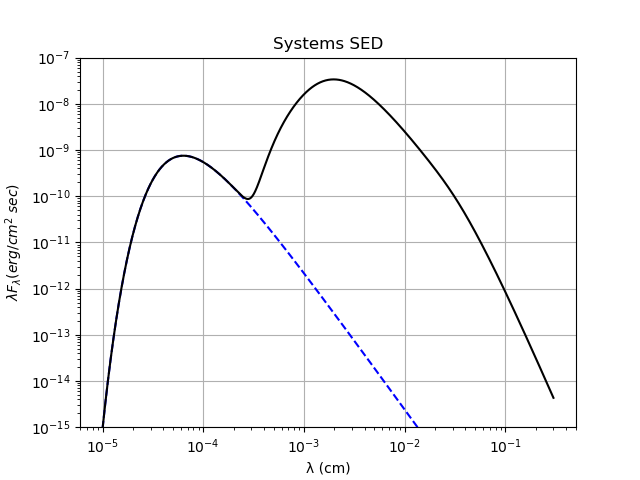
\includegraphics[scale=0.55]{SystemsSED.png}
\caption{Φασματική Κατανομή Ακτινοβολίας του Συστήματος Ήλιου-Δίσκου}\label{fig:SystemSED1}
\end{figure}

Παρακάτω σημειώνεται το όριο απο το οποίο και μετά ανιχνεύεται η παρουσία του δίσκου.


\begin{figure}[h]
\centering
 \begin{subfigure}{0.48\textwidth}
  \centering
  \includegraphics[width=\linewidth]{SystemsSED2.png}
  \caption{{\en System's SED 2}}\label{fig:SystemSED2}
 \end{subfigure}\hfill
 \begin{subfigure}{0.48\textwidth}
  \centering
  \includegraphics[width=\linewidth]{SystemsSED3.png}
  \caption{{\en System's SED 3}}\label{fig:SystemSED3}
 \end{subfigure}
  \caption{Φασματική Κατανομή Ακτινοβολίας του Συστήματος Ήλιου-Δίσκου-2}
\end{figure}


Παρατηρώντας την \ref{fig:SystemSED1} διακρίνουμε δύο κορυφές. Η πρώτη αντιστοιχεί στον αστέρα, ενώ η ύπαρξη της δεύτερης μας φανερώνει ότι πέρα απο το αστέρι του συστήματος υπάρχει και ένας δίσκος μεσοαστρικής ύλης. Η συνάρτηση πηγής του δίσκου είναι μέλαν σώμα, αλλά η αναδυόμενη ειδική ένταση της ακτινοβολίας του, σε αντίθεση με του αστεριού, είναι πολλαπλασιασμένη με τον όρο του οπτικού βάθους \ref{eq:MonochromaticFlux}. Ακόμα η δεύτερη κορυφή είναι μετατοπισμένη σε μεγαλύτερα μήκη κύματος λόγω της πολύ μικρότερης θερμοκρασίας της μεσοαστρικής ύλης του δίσκου.\\

Στην γραφική παράσταση της {\en SED} υπολογίζουμε το γινόμενο $\lambda F_{\lambda}$ και όπως αναφέραμε, ο δισκος εκπέμπει πιο αποτελεσματικά στα μεγάλα μήκη κύματος. Σαν αποτέλεσμα έχουμε μεγαλύτερη μετατόπιση προς τα θετικά του άξονα $y$ του τμήματος που αντιστοιχεί στον δίσκο έναντι αυτού που αντιστοιχεί στον αστέρα. Αυτό φανερώνεται και απο το διάγραμμα μονοχρωματικής ροής, $F_{\lambda} vs \lambda$ του συστήματος, όπου δεν πολλαπλασιάζεται η μονοχρωματική ροή με το μήκος κύματος:

\begin{figure}[h]
\centering
  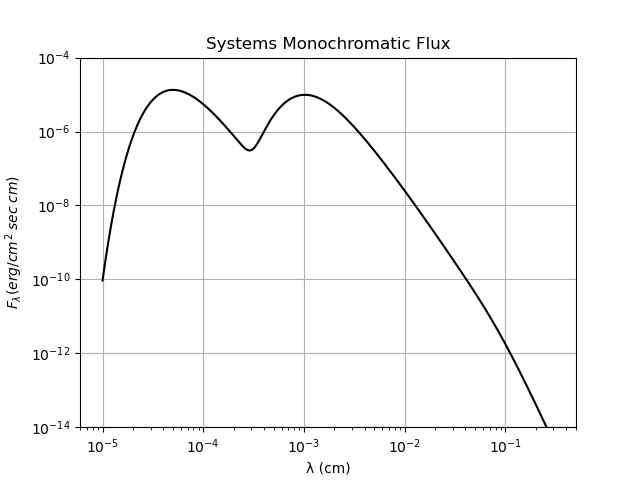
\includegraphics[scale=0.55]{SystemMonochromaticFlux.png}
\caption{Μονοχρωματική ροή ακτινοβολίας του συστήματος}\label{fig:SystemMonochromaticFlux}
\end{figure}


Στο σημείο αυτό πρέπει να αναλογιστούμε μια βασική υπόθεση που κάναμε για την απλοποίση του μοντέλου μας. Για τον υπολογισμό της {\it Θερμοκρασίας Ισορροπίας} της σκόνης θεωρήσαμε ότι {\bf ο δίσκος είναι οπτικά διαφανής} και κατ' επέκταση ότι η ακτινοβολία που απορροφάνε και επανεκπέμπουν τα σωματίδια της σκόνης δεν αποκόπτεται απο άλλα σωματίδια που πιθανώς βρίσκονται μπροστά απο τα πρώτα. Η παραπάνω υπόθεση καταλήγει στις μέγιστες θερμοκρασίες που μπορεί να έχει η σκόνη υπό την ακτινοβολία του συγκεκριμένου αστεριού άρα και στη μέγιστη μονοχρωματική ροή ακτινοβολίας που μπορεί να εκπέμψει αυτός ο δίσκος. Μια πιο αυστηρή ανάλυση του προβλήματος απαιτεί την λύση της διάδοσης της ακτινοβολίας μέσα στον δίσκο. \\

Παρακάτω δίνονται οι γραφικές παραστάσεις της μονοχρωματικής ροής του αστέρα και του δίσκου, για 1000 σημεία με $\lambda$ απο $0.1$μ$m$ έως $3000mm$ (σε λογαριθμική κλιμακα), δίνονται παρακάτω:

\begin{figure}[h]
\centering
 \begin{subfigure}{0.48\textwidth}
  \centering
  \includegraphics[width=\linewidth]{SunMonochromaticFlux.png}
  \caption{Φασματική Κατανομή Ακτινοβολίας του Ήλιου}\label{fig:SunMonochromaticFlux}
 \end{subfigure}\hfill
 \begin{subfigure}{0.48\textwidth}
  \centering
  \includegraphics[width=\linewidth]{DiscMonochromaticFlux.png}
  \caption{Φασματική Κατανομή Ακτινοβολίας του Δίσκου}\label{fig:DiscMonochromaticFlux}
 \end{subfigure}
\end{figure}

και δίνονται αντίστοιχα σε $mJy$, μέσω του {\en script: {\it FluxmJy.py}}:

\begin{figure}[h]
\centering
 \begin{subfigure}{0.48\textwidth}
  \centering
  \includegraphics[width=\linewidth]{SunMonchromaticFluxJY.png}
  \caption{Φασματική Κατανομή Ακτινοβολίας του Ήλιου σε {\en mJy}}\label{fig:SunFluxJy}
 \end{subfigure}\hfill
 \begin{subfigure}{0.48\textwidth}
  \centering
  \includegraphics[width=\linewidth]{DiscMonchromaticFluxJY.png}
  \caption{Φασματική Κατανομή Ακτινοβολίας του Δίσκου σε {\en mJy}}\label{fig:DiscFluxJy}
 \end{subfigure}
\end{figure}

Το εμβαδόν της καμπύλης των διαγραμμάτων μας δίνει την συνολική ροή του αστέρα και του δίσκου αντίστοιχα στην απόσταση των $100pc$ (\ref{eq:FluxBolMon}).
Η συνολική ροή για τον Ήλιο προκύπτει $1.027\times10^{-9} \frac{erg}{sec \; cm^2}$, ενώ για τον δίσκο $5.173\times10^{-8} \frac{erg}{sec \; cm^2}$. Βλέπουμε δηλαδή ότι η ροή του δίσκου φαίνεται να είναι $\sim50$ φορές μεγαλύτερη απο του αστέρα.\\

Αν θυμηθούμε το προφίλ της επιφανειακής πυκνότητας του δίσκου, \ref{fig:SurfDens}, βλέπουμε ότι η μάζα στον δίσκο κατανέμεται με τέτοιον τρόπο ώστε το 55.25\% της συνολικής μάζας του δίσκου βρίσκεται μεταξύ $1-5 AU$, δηλαδή σε έναν δακτύλιο εύρους $~4AU$. Προφανώς και όταν μια τόσο μεγάλη μάζα σκόνης ($5.525\times10^{-4} Μ_{\odot}$) κατανέμεται σε μια τόσο μικρή περιοχή η προσέγγιση του μικρού οπτικού βάθους ξεκινάει να κλονίζεται. Ακόμα παρατηρώντας το προφίλ κατανομής των θερμοκρασιών του δίσκου, \ref{fig:DiscTemp}, βλέπουμε ότι η παραπάνω περιοχή του δίσκου αντιστοιχεί και στην περιοχή με τις μεγαλύτερες θερμοκρασίες. Έτσι ενώ μια {\it ομοιόμορφη} αύξηση της μάζας του δίσκου αυξάνει αναλογικά την ροή, η ταυτόχρονη αύξηση του οπτικού βάθους θα έπρεπε να μειώνει την θερμοκρασία ισορροπίας της σκόνης. Απο την εξίσωση \eqref{eq:TotalPossitiveFlux} βλεπουμε ότι η ροή εξαρτάται εκθετικά απο την θερμοκρασία, οπότε ακόμα και μια μικρή διόρθωση στην τιμή της θερμοκρασίας επηρεάζει σημαντικά την ροη.\\

Στο σημείο αυτό χωρίσαμε τον δίσκο σε δύο περιοχές απο $1-5AU$ και απο $5-20.4AU$ και μετρήσαμε την μονοχρωματική ροή του κάθε τμήματος προσεγγίζοντας τα σαν δύο διαφορετικά σώματα απο το εμβαδόν της κάθε καμπύλης. Παρακάτω δίνονται οι γραφικές παραστάσεις της μονοχρωματικής ροής των δύο περιοχών αντίστοιχα:

\begin{figure}[h]
\centering
 \begin{subfigure}{0.48\textwidth}
  \centering
  \includegraphics[width=\linewidth]{Disc0-5AUMonochromaticFlux.png}
  \caption{Μονοχρωματική ροή ακτινοβολίας απο το κομμάτι του δίσκου 0-5{\en AU}}\label{fig:DiscMonochromaticFlux1stPart}
 \end{subfigure}\hfill
 \begin{subfigure}{0.48\textwidth}
  \centering
  \includegraphics[width=\linewidth]{Disc5-20AUMonochromaticFlux.png}
  \caption{Μονοχρωματική ροή ακτινοβολίας απο το κομμάτι του δίσκου 5-20.4{\en AU}}\label{fig:DiscMonochromaticFlux2ndPart}
 \end{subfigure}
\end{figure}

Οι συνολικές ροές που μετρήθηκαν είναι $1.6\times10^{-8} \frac{erg}{sec \; cm^2}$ και $3.57\times10^{-8} \frac{erg}{sec \; cm^2}$ για το πρώτο και το δεύτερο τμήμα αντίστοιχα. Βλέπουμε ότι η ροή απο το δεύτερο τμήμα είναι $\sim2.23$ φορές μεγαλύτερη απο αυτή του πρώτου! Αρκεί να αναλογιστούμε το εξης:\\

Εάν ο δίσκος ήταν \underline{απόλυτα οπτικά διαφανής} θα έπρεπε το πρώτο κομμάτι του έχοντας μεγαλύτερη μέση θερμοκρασία και ταυτόχρονα μεγαλύτερη επιφανειακή πυκνότητα να έχει μεγαλύτερη ροή. Ο λόγος που αυτό δεν παρατηρείται προδίδεται απο τις εξίσωσεις \ref{eq:MonochromaticFlux} και \ref{eq:OpticalDepth3}, όπου οι μεγάλες τιμές επιφανειακής πυκνότητας σε συνδυασμό με την μικρότερη ροή σε σχέση με το δεύτερο κομμάτι του δίσκου μας λέει ότι τελικά {\it δεν και τόσο οπτικά διαφανής} και μάλιστα το πρώτο κομμάτι είναι περισσότερο αδιαφανή απο το δεύτερο. Ουσιαστικά επιβεβαιώνεται ότι η προσέγγιση του μικρού οπτικού βάθους εισάγει ένα σφάλμα στην μέτρηση της θερμοκρασίας ισορροπίας της σκόνης, το οποίο είναι μεγαλύτερο για το πρώτο κομμάτι του δίσκου και μικρότερο για το δεύτερο.\\

Όσον αφορά την ροή που λαμβάνουμε απο τον Ήλιο, μπορούμε να επαληθεύσουμε την τιμή της. Το μέγιστο της γραφικής παράστασης \ref{fig:SunMonochromaticFlux} αντιστοιχεί στο $\lambda = 0.000050002 cm = 0.5002$μ$m$ και απο τον νόμο του {\en Wien}, \eqref{eq:WienLaw},  προκύπτει η θερμοκρασία του 'Ηλιο $T_{Sun}= 5793.68 K$. Η τιμή είναι πολύ κοντά στην τιμή, \ref{eq:SunsTemp}, που μετρήσαμε και η απόκλιση της προκύπτει απο το γεγονός ότι εδώ εξετάσαμε την μονοχρωματική ροή σε συγκεκριμένο εύρος μηκών κύματος και όχι την βολομετρική που αντιστοιχεί σε όλο το φάσμα. Ακόμα απο το εμβαδόν του ολοκληρώματος υπολογίσαμε ότι η μονοχρωματική ροή του Ήλιου στα $100pc$ είναι $1.027\times10^{-9} \frac{erg}{sec \; cm^2}$. Απο την \ref{eq:Brightness2} και \ref{eq:TotalInteBlackBody} για $100pc$ προκύπτει:

\begin{align*}
\frac{L_\odot}{4\pi (100 pc)^2} = \pi F_\lambda \Rightarrow\\
F_\lambda = \frac{3.8412 \times 10^{33}}{4\pi^2\times(100\times206265\times1.4959^{13})^2} \Rightarrow\\
F_\lambda = 1.022\times10^{-9} \frac{erg}{sec \; cm^2}
\end{align*}

όπου η τιμή μας επαληθεύεται με πάρα πολυ καλή ακρίβεια. \\

Συνοψίζοντας, βλέποντας και μόνο την {\en SED} \ref{fig:SystemSED1} μπορούμε να πούμε τα εξής:

\begin{itemize}

\item Η μορφή της {\en SED} προδίδει την ύπαρξη πρωτοπλανητικού δίσκου γύρω απο τον αστέρα.
\item O πρωτοπλανητικός δίσκος έχει μικρότερη μέση θερμοκρασία απο τον αστέρα.
\item O πρωτοπλανητικός δίσκος εκπέμπει το μεγαλύτερο μέρος της ενέργειας του στα μεγαλύτερα μήκη κύματος.
\item Η υπόθεση οπτικής διαφάνειας οδηγεί στις μέγιστες θερμοκρασίες για τον δίσκο και κατ' επέκταση στην μέγιστη εκπεμπόμενη μονοχρωματική ροή.
\end{itemize}
\newpage


\section{Κατανομή Λαμπρότητας}

Παρατηρώντας την {\en SED} του συστήματος, \ref{fig:SystemSED1}, εντοπίζουμε την ύπαρξη του δίσκου με τα χαρακτηριστικά που αναφέρθηκαν, αλλα η παρουσία του πλανήτη δεν είναι ακόμα προφανής. Όπως αναφέρθηκε στο κεφάλαιο 3, η <<υπογραφή>> της ύπαρξης του πλανήτη είναι η ύπαρξη συντονισμών μέσης κίνησης αλλά και ο κενός δακτύλιος που δημιουργεί στην τροχιά του σε συνδυασμό με την μη ισοτροπική κατανομή των {\en test paticles} κοντά στην απόσταση $r$ του πλανήτη. Κατ' επέκταση οι δύο ομάδες των {\en test particles} που ακολουθούν την τροχιά του (που βρίσκονται σε συντονισμό $1:1$ με αυτόν) και εντοπίζονται στα {σημεία ευσταθούς ισορροπίας {\en Lagrange}} $L_4$ και $L_5$. Στο σημείο αυτό θα προσπαθήσουμε να δημιουργήσουμε δισδιάστατες απεικονίσεις του συστήματος μέσω  της μονοχρωματικής ακτινοβολίας που λαμβάνουμε σε διάφορες συχνότητες παρατήρησης, ώστε να αναδείξουμε αυτην την γεωμετρία του σύστηματος και να έχουμε άμεση απόδειξη της ύπαρξης του πλανήτη.\\

Για την δημιουργία των απεικονίσεων ή <<φωτογραφιών>> συντάχθηκε ένα {\en script} με την ονομασία {\en {\it 2DImageArcsecAU.py}}, όπου χωρίσαμε τον δίσκο σε {\en ``pixels``}, αριθμού $i \times j$ και διαστάσεων $\Delta x^i$, $\Delta y^j$. Φυσικά όσο μεγαλύτερος είναι ο αριθμός των {\en ``pixels``} τόσο μικρότερο είναι και το μέγεθος τους. Ο αριθμός τους δεν μπορεί να είναι απεριόριστα μεγάλος καθώς αυτό θα συνεπάγεται ελάχιστο έως μηδενικό αριθμό σωματιδίων εντός του κάθε {\en ``pixel``} εισάγοντας με αυτόν τον τρόπο ένα στατιστικό σφάλμα. Στη συνέχεια μετρήσαμε όχι μόνο την μέση θερμοκρασία του κάθε {\en ``pixel``} η οποία εξαρτάται μόνο απο την απόσταση του απο το κέντρο του δίσκου \eqref{eq:DustTemp}, αλλά και όλα τα {\en test particles} εντός αυτών. Έπειτα γνωρίζοντας την επιφάνεια του κάθε {\en ``pixel``}, τον αριθμό των {\en test particles} εντός αυτού αλλα και την μάζα του κάθε {\en test particle} \eqref{eq:InitialTPMass} υπολογίσαμε την επιφανειακή πυκνότητα μάζας του κάθε {\en ``pixel``}. Έτσι η μονοχρωματική ροή του κάθε {\en ``pixel``} ($mJy$), σε συνδυασμό με την \eqref{eq:MonochromaticFlux}, δίνεται ώς:

\begin{equation}\label{eq:PixelFlux}
  F_{\nu}^{[i,j]} = (\frac{\Delta x^i \Delta y^j}{D^2})(1-e^{-\tau_{\nu}^{[i,j]}})B_{\nu}(Τ_{dust}^{[i,j]})
\end{equation}
και
\begin{equation}\label{eq:OpticalDepth4}
  \tau_{\nu,[i,j]} = 0.3821 (\frac{\nu}{\nu_0})^{2} \Sigma_{[i,j]},\; \text{όπου $\Sigma_{[i,j]}$ σε $\frac{g}{cm^{2}}$}
\end{equation}

Είναι σύνηθες να βλέπουμε την μονοχρωματική ροή σε μονάδες  $mJy/beam$, όπου $beam$ είναι η συνθετική ακτίνα του ραδιοτηλεσκοπίου εντός της οποίας γίνεται η μέτρηση. Στην συγκεκριμένη εργασία χρησιμοποιήσαμε μια $Gaussian \; beam$, το μέγεθος της οποίας καθορίζεται απο το {\en FWHM} και δίνεται σε $arcsec$. Το μέγεθος της ακτίνας δίνεται απο την \eqref{eq:GaussianBeam} και για τον λόγο αυτό το {\en {\it 2DImageArcsecAU.py}} συντάχθηκε με τέτοιο τρόπο ώστε να μας δίνει τη δυνατότητα να μετράμε το μέγεθος των {\en ``pixels``} είτε σε $AU$ είτε σε $arcsec$. Για να πάμε απο $mJy$ σε $mJy/beam$ ξεκινάμε απο την \eqref{eq:PixelFlux}:

\begin{align}
 F_{\nu}^{[i,j]} = (\frac{\Delta x^i \Delta y^j}{D^2})(1-e^{-\tau_{\nu}^{[i,j]}})B_{\nu}(Τ_{dust}^{[i,j]}) \; \text{$mJy$}\\
 F_{\nu}^{[i,j]} = \frac{\Delta\Omega_b(1-e^{-\tau_{\nu}^{[i,j]}})B_{\nu}(Τ_{dust}^{[i,j]})}{ 4.25\times10^{10}} \; \text{$mJy/beam$}
\end{align}\label{eq:PixelFluxBeam}
όπου $1 steradian = 4.25\times10^{10} (arcsec)^2$.

Τα διάφορα μεγέθη της συνθετικής δέσμης που χρησιμοποιήθηκαν για τις απεικονίσεις του δίσκου δίνονται στον πίνακα \ref{tab:ALMA}. Επιλέξαμε τις μικρότερες δυνατές τιμές του {\en FWHM} για τις διάφορες συχνότητες χωρίς όμως να αποκόπτουμε μέρος του δίσκου. Αυτο σημαίνει ότι φροντίσαμε ώστε η $\vartheta_{MRS}$ να είναι μεγαλύτερη απο την ακτινική διάμετρο του δίσκου ($\vartheta_{MRS}\geq0.408 arcsec$). Η επιλογή της στενής δέσμης γίνεται κατανοητή αν αναλογιστούμε το εξής: Απο την στιγμή που ο δίσκος χωρίστηκε σε {\en ``pixels``}, αριθμού $i \times j$ και διαστάσεων $\Delta x^i$, $\Delta y^j$, το μέγεθος του κάθε {\en pixel} σε $arcsec$ είναι γνωστό. Το εύρος του κενού δακτυλίου στον δίσκο αντιστοιχεί σε κάποιο αριθμό {\en ``pixels``} και κατ' επέκταση σε μια τιμή σε $arcsec$. Ακόμα το εύρος της δέσμης, σε $arcsec$, για τις διάφορες συχνότητες είναι επίσης γνωστό απο την \eqref{eq:GaussianBeam} και τον πίνακα \ref{tab:ALMA}. Έτσι, αφού η τελική εικόνα που προκύπτει είναι η {\it συνέλιξη της δέσμης του ραδιοσυμβολόμετρου με την διασδιάστατο πίνακα μονοχρωματικής ροής}, αν το μέγεθος της δέσμης είναι μικρότερο ή οριακά ίσο με το εύρος του κενού δακτυλίου, τότε αυτός θα είναι απόλυτα ορατός. Στην περίπτωση που η δεσμη είναι μεγαλύτερη απο τον κενό δακτύλιο η διαδικασία της συνέλιξης θα δώσει μια εικόνα στην οποία ο κενός δακτύλιος θα είναι λιγότερο ορατός ή μπορεί να μην είναι και καθόλου ορατός, διότι θα υπάρχει κάποια τιμή μονοχρωματικής ροής στα συγκεκριμένα {\en ``pixels``} λόγω του {\en averaging} που γίνεται εντός της δέσμης. Ακόμα θα πρέπει να προσέξουμε ώστε το μέγεθος της δέσμης να αντιστοιχεί τουλαχιστον σε 16 {\en ``pixels``}, ώστε να μην χάνεται πληροφορία λόγω φτωχής <<ψηφιοποίησης>> της δέσμης συνέλιξης. Η εκλογή περισσότερων {\en ``pixels``} συνεπάγεται την καλύτερη αναπαράσταση της συνθετικής δέσμης του ραδιοτηλεσκοπίου με την οποία συνελίσουμε την πρωτογεννή εικόνα. Παρακάτω δίνονται εικόνες του δίσκου, στις διάφορες τιμές συχνότητας , αλλά και για τα αντίστοιχα μεγέθη της δέσμης που αναγράφονται στον πίνακα \ref{tab:ALMA} πριν και μετα την συνέλιξη με την δέσμη:

\begin{figure}[h]
\centering
 \begin{subfigure}{0.33\textwidth}
  \centering
  \includegraphics[width=\linewidth]{870Unconv.png}
  \caption{{\en Unconvolved Disc at 100pc}}\label{fig:870gHzUnconvolved}
 \end{subfigure}\hfill
 \begin{subfigure}{0.33\textwidth}
  \centering
  \includegraphics[width=\linewidth]{870Conv.png}
  \caption{{\en Disc at 100pc}}\label{fig:870gHzCOnvolved}
 \end{subfigure}\hfill
 \begin{subfigure}{0.33\textwidth}
  \centering
  \includegraphics[width=\linewidth]{870ConvLog.png}
  \caption{{\en Disc at 100pc-Log Flux Density}}\label{fig:Log870gHzCOnvolved}
 \end{subfigure}\hfill
  \caption{Απεικόνιση του δίσκου απόστασης $100pc$ στα $870GHz$}
\medskip
\centering
 \begin{subfigure}{0.33\textwidth}
  \centering
  \includegraphics[width=\linewidth]{650Unconv.png}
  \caption{{\en Unconvolved Disc at 100pc}}\label{fig:650gHzUnconvolved}
 \end{subfigure}\hfill
 \begin{subfigure}{0.33\textwidth}
  \centering
  \includegraphics[width=\linewidth]{650Conv.png}
  \caption{{\en Disc at 100pc}}\label{fig:650gHzCOnvolved}
 \end{subfigure}\hfill
 \begin{subfigure}{0.33\textwidth}
  \centering
  \includegraphics[width=\linewidth]{650ConvLog.png}
  \caption{{\en Disc at 100pc-Log Flux Density}}\label{fig:Log650gHzCOnvolved}
 \end{subfigure}\hfill
  \caption{Απεικόνιση του δίσκου απόστασης $100pc$ στα $650GHz$}
\end{figure}

\newpage

\begin{figure}[h]
\centering
 \begin{subfigure}{0.33\textwidth}
  \centering
  \includegraphics[width=\linewidth]{460Unconv.png}
  \caption{{\en Unconvolved Disc at 100pc}}\label{fig:460gHzUnconvolved}
 \end{subfigure}\hfill
 \begin{subfigure}{0.33\textwidth}
  \centering
  \includegraphics[width=\linewidth]{460Conv.png}
  \caption{{\en Disc at 100pc}}\label{fig:460gHzCOnvolved}
 \end{subfigure}\hfill
 \begin{subfigure}{0.33\textwidth}
  \centering
  \includegraphics[width=\linewidth]{460ConvLog.png}
  \caption{{\en Disc at 100pc-Log Flux Density}}\label{fig:Log460gHzCOnvolved}
 \end{subfigure}\hfill
  \caption{Απεικόνιση του δίσκου απόστασης $100pc$ στα $460GHz$}
\medskip
\centering
 \begin{subfigure}{0.33\textwidth}
  \centering
  \includegraphics[width=\linewidth]{325Unconv.png}
  \caption{{\en Unconvolved Disc at 100pc}}\label{fig:325gHzUnconvolved}
 \end{subfigure}\hfill
 \begin{subfigure}{0.33\textwidth}
  \centering
  \includegraphics[width=\linewidth]{325Conv.png}
  \caption{{\en Disc at 100pc}}\label{fig:325gHzCOnvolved}
 \end{subfigure}\hfill
 \begin{subfigure}{0.33\textwidth}
  \centering
  \includegraphics[width=\linewidth]{325ConvLog.png}
  \caption{{\en Disc at 100pc-Log Flux Density}}\label{fig:Log325gHzCOnvolved}
 \end{subfigure}\hfill
  \caption{Απεικόνιση του δίσκου απόστασης $100pc$ στα $325GHz$}
  \medskip
\centering
 \begin{subfigure}{0.33\textwidth}
  \centering
  \includegraphics[width=\linewidth]{230Unconv.png}
  \caption{{\en Unconvolved Disc at 100pc}}\label{fig:230gHzUnconvolved}
 \end{subfigure}\hfill
 \begin{subfigure}{0.33\textwidth}
  \centering
  \includegraphics[width=\linewidth]{230Conv.png}
  \caption{{\en Disc at 100pc}}\label{fig:230gHzCOnvolved}
 \end{subfigure}\hfill
 \begin{subfigure}{0.33\textwidth}
  \centering
  \includegraphics[width=\linewidth]{230ConvLog.png}
  \caption{{\en Disc at 100pc-Log Flux Density}}\label{fig:Log230gHzCOnvolved}
 \end{subfigure}\hfill
  \caption{Απεικόνιση του δίσκου απόστασης $100pc$ στα $230GHz$}
\end{figure}

Βλέποντας τις παραπάνω εικόνες μπορούμε να κατανοήσουμε την σημασία της μεγάλης  διακριτικής ικανότητας για την ανάδειξη της γεωμετρίας του δίσκου με μεγαλύτερη λεπτομέρεια. Αν δούμε την περίπτωση της απεικόνισης στα $325GHz$, όπου έχουμε πολύ στενή δέσμη, ο κενός δακτύλιος είναι αρκετά εμφανής. Στην περίπτωση όμως της απεικονίσεως των $650GHz$ το εύρος της δέσμης είναι $\sim1.7$ φορές μεγαλύτερο$\cdot$ με αποτέλεσμα ο κενός δακτύλιος να είναι λιγότερο εμφανής.\\

Η ικανότητα μας να απεικονίσουμε τον κενό δακτύλιο με μεγαλύτερη λεπτομέρεια δεν σταματάει εδώ. Ας υποθέσουμε ότι έχουμε την παραπάνω εικόνα του δίσκου στα $325GHz$, η οποία απο μόνη της είναι ένα πολύ ισχυρό επιχείρημα για την ύπαρξη πλανήτη. Βλεπουμε ότι ο κενός δακτύλιος βρίσκεται εντός μιας γωνιακής διαμέτρου  $\sim 1 arcsec$ και απο τον πινακα \ref{tab:ALMA} βλεπουμε ότι $\vartheta_{MRS} = 0.418 arcsec$. Σαν αποτέλεσμα αν είχαμε πραγματικά την δυνατότητα χειρισμού του {\en ALMA} μετά την απεικόνιση του πλήρη δίσκου θα μπορούσαμε να επιλέξουμε ακόμα μικροτερες διακριτικές ικανότητες (με $\vartheta_{MRS} < 0.408 arcsec$) αποκόπτοντας μεν τα εξωτερικά όρια του δίσκου, αλλά λαμβάνοντας μεγαλύτερη λεπτομέρεια στην απεικόνιση του κενού το οποίο βρίσκεται εντός $\vartheta_{MRS}$. Ουσιαστικά στην περίπτωση αυτή το ραδιοσυμβολόμετρο αποκόπτει την μονοχρωματικη ροή που έρχεται απο $\vartheta_{MRS}$ και πάνω και σαν αντάλλαγμα παρέχει μεγαλύτερη διακριτική ικανότητα στην απεικόνιση της περιοχής $\vartheta_{MRS}$ και κάτω.\\

Μια ακόμα σημαντική βελτίωση στην λεπτομέρεια της εικόνας μπορεί να εισέλθει αυξάνοντας τον αριθμό των {\en ``pixels``} της εικόνας. Όπως αναφέραμε όσο μεγαλώνει ο αριθμός αυτός όλο και λιγότερα σωματίδια περιέχονται σε κάθε {\en ``pixel``} αυξάνοντας το στατιστικό σφάλμα στις μετρήσεις. Εύλογα μπορεί να συμπεράνει κανείς ότι περιοχές με μικρή επιφανειακή πυκνότητα θα παρουσιάζουν μεγαλύτερο στατιστικό σφάλμα έναντι αυτών με μεγαλύτερη. Στο σημείο αυτό εκμεταλλευόμαστε το ότι ο κενός δακτύλιος και κατ' επέκταση η περιοχή που θέλουμε να απεικονίσουμε είναι η εσωτερική περιοχή του δίσκου και εντοπίζεται σε γωνιακή διαμέτρο $\leq 1 arcsec$. Σαν αποτέλεσμα αυξάνοντας των αριθμό των {\en ``pixels``} της εικόνας αυξάνεται περισσότερο το στατιστικό σφάλμα των περιοχών γωνιακής διαμέτρου $> 1 arcsec$, αλλα οι περιοχές αυτές γίνονται {\en ``filter-out``} λόγω του ορίου που θέτει η $\vartheta_{MRS}$. Παρακάτω δίνονται οι εικόνες του δίσκου στα $325GHz$ και $230GHz$ και τα αντίστοιχα μεγέθη της δέσμης που αναγράφονται στον πίνακα \ref{tab:ALMA2}. Παρέχονται εικόνες μετα την συνέλιξη με την δέσμη:

\begin{figure}[h]
\centering
 \begin{subfigure}{0.48\textwidth}
  \centering
  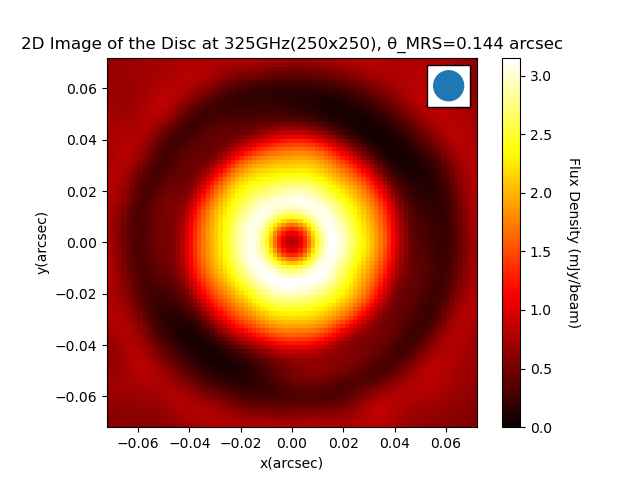
\includegraphics[width=\linewidth]{325ConvThMRS.png}
  \caption{{\en Disc at 100pc}, $\vartheta_{MRS}= 0.144 arcsec$}\label{fig:325ConvThMRS}
 \end{subfigure}\hfill
 \begin{subfigure}{0.48\textwidth}
  \centering
  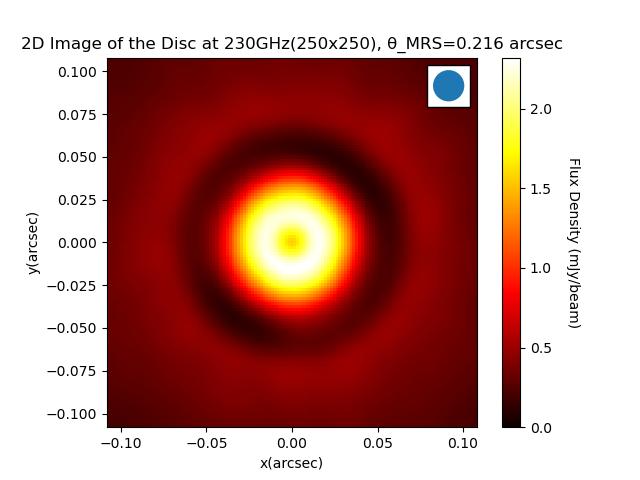
\includegraphics[width=\linewidth]{230ConvThMRS.png}
  \caption{{\en Disc at 100pc}, $\vartheta_{MRS}= 0.216 arcsec$}\label{fig:230ConvThMRS}
 \end{subfigure}\hfill
 \caption{Απεικόνιση εσωτερικού τμήματος του δίσκου απόστασης $100pc$}
\end{figure} 

Στις παραπάνω εικόνες βλέπουμε με πολύ μεγάλη ευκρίνεια τον κενό δακτύλιο, ο οποίος αποτελεί και την \underline{ένδειξη υπαρξης του πλανήτη.} Μάλιστα στην απεικόνιση των $325GHz$, όπου έχουμε και την μεγαλύτερη δυνατή διακριτική ικανότητα, μπορούμε να διακρίνουμε αμυδρά τις δύο ομάδες των αντίστοιχων Τρωικών. Φυσικά θα πρέπει κανείς να σκεφτεί ότι σε μια πραγματική απεικόνιση ενός δίσκου θα υπάρχει και θερμικός θόρυβος, ο οποίος <<θολωνει>> την εικόνα. Σαν αποτέλεσμα οι πραγματικές απεικονίσεις θα είναι πιο θολές και με μικρότερη λεπτομέρεια. Πιθανότατα να μην φαίνονται οι Τρωικοί δορυφόροι, αλλα {\it η ύπαρξη και μόνο του κενού δακτυλίου είναι η <<υπογραφή>> της παρουσίας του γιγάντιου πλανήτη στο σύστημα.}\\

Τέλος μπορεί να παρατηρήσει κανείς ότι τελίκά επιλέξαμε τις μικρότερες συχνότητες για την απεικόνιση του δίσκου και η επιλογή αυτή δεν είναι τυχαία. Αρχικά βλεπουμε ότι το {\en ALMA} μπορεί να πετύχει μεγαλύτερες διακριτικές ικανότητες σε αυτές τις συχνότητες μέσω των {\en Configurations C-10}. Ο δεύτερος και πιο σημαντικός λόγος είναι ότι όπως αποδείξαμε η σκόνη εκπέμπει πιο αποτελεσματικά στα μεγαλύτερα μήκη κύματος έναντι του αστέρα. Μικρότερες συχνότητες ισοδυναμούν με μεγαλύτερα μήκη κύματος, άρα σε μια πραγματική απεικόνιση, όπου θα περιεχόταν και το αστέρι στο κέντρο του δίσκου, η μονοχρωματική ακτινοβολία που θα λαμβάναμε απο αυτό θα είναι σημαντικά μικρότερη έναντι του δίσκου. Σαν αποτέλεσμα είναι δυνατό να εντοπίσουμε τις δομικές λεπτομέρειες του δίσκου χώρις η φασματική κατανομή ακτινοβολίας του αστέρα να κυριαρχεί. Εάν το τελευταίο συνέβαινε τότε θα ήταν αναγκαίες μη πραγματοποιήσιμες απεικονίσεις με μεγάλο δυναμικό εύρος, ώστε να μπορούσε να αποκαλυφθεί ο δίσκος και τα δυναμικά χαρακτηριστικά του, τα οποία μας δείχνουν την ύπαρξη του μαζικού πλανήτη.

\chapter{Παρατηρήσεις και Συμπεράσματα}
Ο στόχος της παρούσας πτυχιακής διατριβής ήταν να εξετάσει την δυναμική αλληλεπίδραση ενός γιγάντιου πλανήτη με έναν πρωτοπλανητικό δίσκο σκόνης, να εξακριβώσει και τελικά να αναδείξει κάποιον <<δείκτη>> που θα αποτελεί την <<υπογραφή>> ύπαρξης του πλανήτη στο σύστημα. Επείδη η ύπαρξη τέτοιων δίσκων γίνεται αντιληπτή μέσω της ισχυρής {\en far-IR/submillimeter} ακτινοβολίας που εκπέμπουν, σαν στόχος ανίχνευσης τέτοιων δεικτών τέθηκε η δημιουργία  απεικόνισεων του δίσκου με τις διακριτικές ικανότητες της {\en ALMA}. Σκοπός των απεικονίσεων ήταν η ανάδειξη του <<δείκτη>> ύπαρξης του πλανήτη, η ποιοτική ανάλυση των εικόνων και εκλογή συμπερασμάτων σχετικά με την πραγματική απεικόνιση τέτοιων δίσκων.\\

Βασικό στοιχείο στην μελέτη μας ήταν η δυναμική εξέλιξη του συστήματος για χρόνικό διάστημα που αντιστοιχεί σε πολλές περιόδους περιφοράς του πλανήτη, ώστε τα αποτελέσματα που θα πάρουμε να είναι ασφαλή. Απο την σκοπιά της {\it δυναμικής ανάλυσης} του προβλήματος είδαμε ότι η παρουσία του πλανήτη επιβεβαιώνεται όχι μόνο απο τον <<κενό>> δακτύλιο, τον οποίο δημιουργεί στο επίπεδο της τροχιάς του, αλλα και απο την δημιουργία των δύο ομάδων (<<Τρωικοί>>) με τους οποίους βρίσκεται σε σταθερό συντονισμό $1:1$ και μοιράζεται την τροχιά του. Είδαμε ότι το εύρος του δακτυλίου εξαρτάται απο την {\it ακτίνα {\en Hill}} του πλανήτη και κατ' επέκταση απο τον λόγο της μάζας του πλανήτη προς την μάζα του αστέρα του συστήματος. Ένα ακόμα σημαντικό συμπέρασμα είναι ότι η  ύπαρξη του πλανήτη μπορεί να ιχνηλατηθεί και σε αποστάσεις αρκετά μεγαλύτερες απο την {\it ακτίνα {\en Hill}} του$\cdot$ μέσω της εμφάνισης συντονισμών μέσης κίνησης. Στην περίπτωση αυτή παρατηρούνται τοπικά ελάχιστα στην αριθμητική πυκνότητα των σωματιδίων της σκόνης σε αποστάσεις που εμπίπτουν στους ασταθείς αυτούς συντονισμούς, καθώς τα στοιχεία της τροχιάς των σωματιδίων μεταβάλλονται έντονα και σε σύντομα χρονικά διαστήματα.\\
Απο την σκοπιά της ανίχνευσης της ηλεκτρομαγνητικής ακτινοβολίας του δίσκου στο {\en far-IR/submillimeter} και τελικά όπως αυτή θα φαινόταν μετά απο χαρτογράφιση με την {\en ALMA} είδαμε ότι ο <<δείκτης>> που επιβεβαιώνει την ύπαρξη του πλανήτη και είναι ανιχνεύσιμος είναι ο <<κενός>> δακτύλιος που δημιουργεί. Στην περίπτωση όμως αυτή, καταλάβαμε ότι η ανιχνευσιμότητα του παραπάνω <<δείκτη>> εξαρτάται απο πολλούς παράγοντες που θα μπορούσαν να καταταχθούν συνοπτικα σε δύο κατηγορίες: 

\begin{enumerate}

\item Φυσικά χαρακτηριστικά του συστήματος Δίσκου-Αστέρα

Αρχικά είδαμε πόσο σημαντική είναι η εκλογή του μοντέλου ακτινοβολίας$\cdot$ καθώς ο πρώτος παράγοντας που καθορίζει τη θέρμοκρασία της σκόνης είναι η βολομετρική ροή του αστέρα. Ταυτόχρονα, ο δεύτερος παράγοντας είναι τα φυσικά χαρακτηριστικά της σκόνης που συγκροτούν τον δίσκο, πιο συγκεκριμένα η σύσταση, το σχήμα και το μέγεθος, αφού προσδιορίζουν όχι μόνο πόση ενέργεια θα απορροφήσει και θα επανεκπέμψει η σκόνη αλλά και σε ποιά μήκη κύματος$\cdot$ ορίζοντας τελικά την θερμοκρασίας ισορροπίας της. Απο την πλευρά της, η τελική θερμοκρασία του δίσκου σε συνδυασμό με την επιφανειακή του πυκνότητα και την απόσταση του καθορίζουν στην τελική ποσότητα μονοχρωματικής ροής που θα φτάσει σε αυτά.

\item Χαρακτηριστικά-Δυνατότητες των οργάνων παρατήρησης

Στην δεύτερη αυτή κατηγορία είδαμε την ποσοτικοποίηση των περιορισμών της διακριτικής ικανότητας των σύγχρονων συμβολομέτρων. Πιο συγκεκριμένα, στα μήκη κύματος που ο δίσκος εκπέμπει αποτελεσματικά σε συνδυασμό με τις τιμές διακριτικής ικανότητας που μπορούν επιτύχουν στις αντίστοιχες συχνότητες. Είδαμε την σημασία των παραπάνω στην περίπτωση ανίχνευσης του <<κενού>> δακτυλίου για το μοντέλο μας, όπου η σχέση μεταξύ διακριτικής ικανότητας και συχνότητας ανίχνευσης ουσιαστικά καθιστούσε το αν ο δείκτης θα ήταν ανιχνεύσιμος σε κάποια απεικόνιση ή όχι.
\end{enumerate}

Στην δημιουργία και μελέτη προσομοιώσεων συστημάτων εξίσου βασικό με την εκλογή συμπερασμάτων είναι και η ικανότητα προσδιορισμού των σημείων όπου το μοντέλο εισάγει περιορισμούς λόγω παροδοχών. Η κατανόηση των περιορισμών αυτών είναι πολύ σημαντική καθώς χαράζει τον δρόμο στον οποίο πρέπει να κινηθούμε βελτιώνοντας το μοντέλο μας και τελικά παράγοντας αποτελέσματα πιο κοντά στον φυσικό κόσμο.\\ 

Στην περίπτωση του μοντέλου μας, όπως αναφέρθηκε, τα {\en test particles} αντιμετωπίζονται ως σωματίδια μηδενικής μάζας απο τον {\en SWIFT}, δεν αλληλεπιδρούν μεταξύ τους και δεν επηρέαζουν βαρυτικά τον πλανήτη. Η παραπάνω συμπεριφορά φυσικά εισάγει ένα σφάλμα στις τελικές τιμές των διανυσμάτων θέσης και ορμής που λαμβανούμε για τα {\en test particles} μετα την ολοκλήρωση των $10Myrs$. Το σφάλμα όμως αυτό δεν επηρεάζει σημαντικά τα αποτελέσματα μας, διότι η αλλαγή των διανυσμάτων θέσης και ορμής των {\en test particles} την χρονική στιγμή $t_1=10Myrs$ δεν αλλάζει το γεγονός της δημιουργίας του κενού δακτυλίου στην τροχιά του πλανήτη. Ακόμα η μάζα του πλανήτη εξακολουθεί να είναι μεγαλυτερη απο αυτή των {\en test particles} κατα 6 τάξεις μεγέθους άρα παραμένει η αντίληψη ότι αυτός επηρεάζει σημαντικά τα {\en test particles} και επηρεάζεται λιγότερο απο αυτά. Ακόμα η παραδοχή του μικρού οπτικού βάθους για τον δίσκο εισάγει, όπως περιγράψαμε, ένα σφάλμα στον υπολογισμό της κατανομής θερμοκρασιών του δίσκου το οποίο έχει ως αποτέλεσμα να λαμβάνουμε τις μεγαλύτερες τιμές ειδικών εντάσεων της ακτινοβολίας απο τον δίσκο. Απο αυτή την άποψη, μαζί με την υπόθεση μεγάλων ποσοτήτων μεσοαστρικής σκόνης για τον δίσκο τα αποτελέσματα μας είναι μαξιμαλιστικά.\\

Συνοψίζοντας, η πραγμάτωση παραδοχών για την δημιουργία προσομοιώσεων του δίσκου είναι αναγκαία$\cdot$ καθώς κανένας κώδικας δεν μπορεί να διαχειριστεί την πολυπλοκότητα τέτοιων συστημάτων ούτε τον αριθμό των σωματιδίων του με πλήρη ταυτίση της πραγματικότητας! Σαν αποτέλεσμα είναι λογικό η υπολογιστική ακρίβεια των αποτελεσμάτων να αποκλίνει σε κάποιο βαθμό απο την πραγματική εικόνα, {\it η ποιοτική όμως συμπεριφόρα του συστήματος μπορεί μελετηθεί με πολύ καλή ακρίβεια δίνοντας μας την δυνατότητα εκλογής συμπερασμάτων για την φυσική συμπεριφορά αυτού}. Το <<στοίχημα>> για τα επόμενα χρόνια είναι η δημιουργία αλγορίθμων που θα μπορούν να διαχειριστούν μεγαλύτερες τιμές σωματιδίων βρίσκοντας τις βαρυτικές δυνάμεις που αναπτύσσονται μεταξύ όλων των σωμάτων του συστήματος. Ακόμα η δημιουργία αλγορίθμων που θα μελετάνε αναλυτικά το πρόβλημα της διάδοσης ακτινοβολίας και της αλληλεπίδρασης της με σωματίδια διαφορετικών μεγεθών, σχημάτων και σύστασης$\cdot$ καθορίζοντας τελικά το προφίλ κατανομής θερμοκρασιών σε διαφορετικούς δίσκους σκόνης με μεγαλύτερη ακρίβεια.


\bibliographystyle{plain}
\en
\bibliography{Bibliography}
\end{document}
